\chapter{The monojet analysis}
    \label{chapter:MonojetAnalysis}

The monojet analysis is described in detail in this chapter.
The data and the Monte Carlo simulated samples used for the analysis are presented, together with the definition of the different physics objects and the event selection criteria.
The statistical treatment of the data and the estimation of the different Standard Model (SM) background processes are discussed.
The observations are then compared to the SM predictions in the different signal regions.


\section{Data sample}
    \label{sec:DataSample}

The data sample considered in the analysis presented in this Thesis was collected with the ATLAS detector in proton-proton collisions at a center of mass energy of $\unit[8]{TeV}$ between April 4, 2012 and December 6, 2012.
A total integrated luminosity of  $\unit[20.3 \pm 0.6]{fb^{-1}}$ was recorded after requiring tracking detectors, calorimeters, muon chambers and magnets to be fully operational during the data taking.
Events are selected using the lowest unprescaled $\met$ trigger logic called \texttt{EF\_xe80\_tclcw}, that selects events with $\met$ above $\unit[80]{GeV}$, as computed at the final stage of the three-level trigger system of ATLAS discussed in Section~\ref{subsec:TriggerSystem}. 
The details of the implementation of the $\met$ trigger can be found in Ref.~\cite{Casadei:2011via}.


\section{Object definition}
    \label{sec:ObjectDefinition}

Jets and $\met$ are used to define the signal selections whereas leptons are used to both veto the electroweak backgrounds and to define the different control samples.


\subsection{Jets}
    \label{subsec:JetDefinition}

Jets are reconstructed from energy deposits in the calorimeters using the $\akt$ jet algorithm with the jet radius parameter $R=0.4$ (see Section \ref{sec:JetReco}).
The transverse momentum of the jets is corrected for detector effects with the LCW calibration.
Jets with corrected $\pt>\unit[20]{GeV}$ and $|\eta|<2.8$ are considered in the analysis.
In order to remove jets originating from pileup collisions, central jets ($|\eta|<2.4$) with $\pt < \unit[50]{GeV}$ are required to have a jet vertex fraction (JVF) above 0.5.


\subsection{Electrons}
    \label{subsec:ElectronDefinition}

Electrons are required to have $\pt>\unit[20]{GeV}$ and $|\eta|<2.47$, and need to fulfill the \emph{medium} shower shape and track selection criteria (see Section \ref{sec:ElectronReco}).
The same $\pt$ threshold is used to veto electrons in the signal selections and to select them in the control samples (see Section~\ref{sec:EventSelection}), which minimizes the impact of the reconstruction, identification and efficiency systematic uncertainties.
The threshold of $\unit[20]{GeV}$ used in this definition combined to the definition of the electron control sample, brings the background of jets misidentified as electrons to negligible levels, and therefore no isolation is required.

Overlaps between identified electrons and jets in the final state are resolved.
Jets are discarded if their separation $\Delta R$ from an identified electron is less than 0.2.
The electrons separated by $\Delta R$ between 0.2 and 0.4 from any remaining jet are removed.


\subsection{Muons}
    \label{subsec:MuonDefinition}

Muons are reconstructed by combining information from the muon spectrometer and inner tracking detectors (see Section~\ref{sec:MuonReco}).
The muon candidates for the analysis presented are required to have $\pt>\unit[10]{GeV}$, $|\eta|<2.4$, and $\Delta R > 0.4$ with respect to any jet candidate with $\pt > \unit[30]{GeV}$.
The use of this $\pt$ threshold increases the precision for selecting real muons from $W$ boson decays, and avoids the bias in the muon selection due to the presence of low $\pt$ jets with large pileup contributions.
Finally, an isolation condition is applied to the muons, that requires the sum of the $\pt$ of the tracks not associated with the muon in a cone of radius $\Delta R = 0.2$ around the muon direction, to be less than $\unit[1.8]{GeV}$.

\subsection{Missing transverse energy}
    \label{subsec:MetDefinition}

The missing transverse energy is described in detail in Section~\ref{subsec:ETmissReco}.
It is reconstructed using all energy deposits in the calorimeter up to a pseudorapidity $|\eta|<4.9$, and without including information from identified muons in the final state.


\section{Event selection}
    \label{sec:EventSelection}

The different signal regions defined in this analysis have a common preselection criteria, that suppresses large contribution of SM processes with leptons in the final state and non-collision background contributions:

\begin{itemize}
\item Events are required to have a reconstructed primary vertex consistent with the beam spot envelope and it is required to have at least five isolated tracks with $\pt>\unit[400]{MeV}$.
If two or more vertices are consistent with these requirements, the one with the largest sum $\pt^2$ is chosen as primary vertex.
This requirement removes beam-related backgrounds and cosmic rays.

\item Events are initially requested to have $\met>\unit[150]{GeV}$ in order to ensure the trigger to be fully efficient.

\item At least one jet with $\pt>\unit[150]{GeV}$ and $|\eta|<2.8$ is required in the final state, in order to select monojet-like configurations.

\item Different quality cuts are applied to remove events recorded during a LAr noise burst or during a failure in the electronics of any subsystem.
Also events not correctly processed are vetoed from the selection.

\item Events containing any jet with $\pt>\unit[20]{GeV}$ and $|\eta|<4.5$ with charged fraction \footnote{The charged fraction is defined as $f_{\text{ch}} = \sum{\pt^{\text{track,jet}}/\pt^{\text{jet}}}$, where $\sum{\pt^{\text{track,jet}}}$ is the scalar sum of the transverse momenta of the tracks associated to the primary vertex within a cone of radius 0.4 around the jet axis, and $\pt^{\text{jet}}$ is the transverse momentum as determined from the calorimetric measurements.}, 
electromagnetic fraction\footnote{The electromagnetic fraction is defined as $f_{\text{em}} = E_{\text{LAr}}/(E_{\text{LAr}} + E_{\text{TileCal}})$, where $E_{\text{LAr}}$ is the energy deposited in the electromagnetic calorimeter and $E_{\text{TileCal}}$ is the energy deposited in the hadronic calorimeter.} 
or sampling fraction\footnote{$f_{\text{max}}$ denotes the maximum fraction of the jet energy collected by a single calorimeter layer.} inconsistent with the requirement that they originate from a $\pp$ collision ($f_{\text{ch}}<0.02$, $f_{\text{em}}<0.1$ and $f_{\text{max}}>0.8$ respectively), are vetoed.

\item Events with one or more reconstructed isolated muons with $\pt>\unit[10]{GeV}$ or electrons with $\pt>\unit[20]{GeV}$ are vetoed.
\end{itemize}

A maximum of three jets with $\pt>\unit[30]{GeV}$ and $|\eta|<2.8$ in the event are allowed.
An additional requirement on the azimutal separation of $\Delta\phi(\text{jet}, \met) > 0.4$ between the missing transverse momentum direction and that of each of the selected jets is imposed.
The latest suppresses the multijet background contribution where the large $\met$ originates from a jet energy mismeasurement.

Three separate signal regions (denoted by M1, M2 and M3) are defined with increasing lower thresholds on the leading jet $\pt$ and $\met$.
The definition of these signal regions come as a result of an optimization on the stop pair production with $\stoptocharm$ model, performed across the stop-neutralino mass plane with increasing $\stopone$ and $\ninoone$ masses.

For the M1 selection, the events are required to have $\met>\unit[220]{GeV}$ and leading jet $\pt>\unit[280]{GeV}$. M2 (M3) selection must have $\met>\unit[340]{GeV}$ ($\met>\unit[450]{GeV}$) and leading jet $\pt>\unit[340]{GeV}$ ($\pt>\unit[450]{GeV}$).

Three extra generic signal regions (M4, M5 and M6) are defined to increase the sensitivity to a broad variety of models leading to final states with larger $\met$. Signal region M4 requires the events to have leading jet $\pt>\unit[450]{GeV}$ and $\met>\unit[340]{GeV}$, while region M5 (M6) are required to have leading jet $\pt>\unit[550]{GeV}$ and $\met>\unit[550]{GeV}$ (leading jet $\pt>\unit[600]{GeV}$ and $\met>\unit[600]{GeV}$).
Table \ref{tab:SignalRegionCuts} summarizes the six signal region selections.

\begin{table}[!ht]
  \renewcommand{\baselinestretch}{1}
  \begin{center}
    \begin{small}
      \begin{tabular*}{\textwidth}{@{\extracolsep{\fill}}lcccccc}\hline\hline
        \multicolumn{7}{c}{\small{\textbf{Selection criteria}}} \\\hline
        %%% --- PRESELECTION
        \multicolumn{7}{c}{{\small{Preselection}} } \\\hline
        \multicolumn{7}{l}{Primary vertex}\\
        \multicolumn{7}{l}{$\met > 150$~GeV }\\
        \multicolumn{7}{l}{At least one jet with $\pt >150$~GeV and $|\eta|< 2.8$}\\
        \multicolumn{7}{l}{Jet quality requirements}   \\
        \multicolumn{7}{l}{Lepton vetoes}\\ \hline
        %%% --- MONOJET
        \multicolumn{7}{c}{\small{Monojet-like selection}}\\\hline
        \multicolumn{7}{l}{At most a total of three jets with $\pt > 30$~GeV and $|\eta|<2.8$}\\
        \multicolumn{7}{l}{$\Delta\phi(\text{jet}, \met) > 0.4$} \\\hline
        Signal region                   & M1  & M2  & M3  & M4  & M5  & M6  \\
        Minimum leading jet $\pt$ [GeV] & 280 & 340 & 450 & 450 & 550 & 600 \\
        Minimum $\met$ [GeV]            & 220 & 340 & 450 & 340 & 550 & 600 \\ \hline\hline
      \end{tabular*}
    \end{small}
  \end{center}
  \caption{Event selection criteria applied for the signal regions M1 to M6.}
  \label{tab:SignalRegionCuts}
\end{table}


\section{Monte Carlo simulated samples}
    \label{sec:MCSamples}

The analysis uses MC samples to estimate each Standard Model process.
The MC events are passed through a detailed simulation of the detector based on {\sc Geant4} \cite{Agostinelli:2002hh}.
Different in-time and out-of-time pileup conditions as a function of the instantaneous luminosity are also taken into account by overlaying simulated minimum-bias events generated with \pythia-8 onto the hard scattering process and re-weighting them with the distribution of the observed mean number of interactions per bunch crossing.

In the following, details are given for the SM background MC simulated samples.


\subsection{$W$+jets and $Z$+jets}
    \label{subsec:WZjetsMCSimulation}

A set of simulated $W$+jets and $Z$+jets events are generated using \sherpa{}, including LO matrix elements for up to 5 partons in the final state and using massive $b/c$-quarks, CT10 parton distribution functions\footnote{Next-to-next-to-leading order (NNLO) PDFs from the CTEQ/TEA group.} and its own model of hadronization.
Similar samples have been generated with the \alpgen{} generator, to study the modeling uncertainties.
The MC samples are initially normalized to next-to-next-to-leading-order (NNLO) cross sections in perturbative QCD (pQCD) with the DYNNLO \cite{Catani:2007vq} program using MSTW2008 NNLO PDF sets.


\subsection{Top} 
    \label{subsec:TopSimulation}

The production of top quark pairs (\ttbar) is simulated using the \powheg{} MC generator.
A top quark mass of $\unit[172.5]{GeV}$, the CTEQ6L1 parton distribution functions and the Peruggia 2011C Tune \cite{Skands:2010ak} have been used for the generation and the underlying event simulation.
The $\ttbar$ samples are normalized to NNLO+NNLL (next-to-next-to-leading-logarithm pQCD accuracy), determined by \texttt{Top++2.0}.
Similar \alpgen{} and \mcnlo{} samples are used to assess the $\ttbar$ modeling uncertainties.

Single top samples are generated with \powheg{} for the $s$- and $Wt$-channels, while \acer{} \cite{Kersevan:2002dd} is used for the $t$-channel.
An approximate NLO+NNLL pQCD prediction is used for the $Wt$ process.
Samples generated with the \mcnlo{} generator are then used to estimate the systematic uncertainties.

\subsection{Diboson}
    \label{subsec:DibosonSimulation}

Diboson samples ($WW$, $WZ$ and $ZZ$ production) are generated with \sherpa{}, using massive $c$/$b$-quarks, with CT10 PDF and are normalized to NLO predictions.
Similar samples generated with \herwig{} are used to compute the modeling uncertainties.



\section{Background estimation}
    \label{sec:BkgEstimation}

The expected SM background is dominated by $\znn$ (irreducible), $\wln$ and $\ttbar$ production, and includes small contributions from $\zgammall$, single top, diboson and multijet processes.

The $W/Z$+jets backgrounds are estimated using MC event samples normalized using data in control regions.
The simulated $W/Z$+jets events are re-weighted to data as a function of the generated $\pt$ of the vector boson, which is found to improve the agreement between data and simulation.
The weights are extracted from the comparison of the reconstructed boson $\pt$ distribution in data and {\sherpa} MC simulation in a $W$+jets control sample where the jet and $\met$ preselection requirements from Table \ref{tab:SignalRegionCuts} have been applied.
As detailed in Appendix~\ref{app:BosonPtReweight}, these weights are defined in several bins in the boson $\pt$ and applied to the truth boson $\pt$ distribution of the simulated samples.
Due to the limited number of data events at large boson $\pt$, an inclusive last bin with boson $\pt > \unit[400]{GeV}$ is used.
The uncertainties of the re-weighting procedure are taken into account in the final result.

The top-quark background contribution is very small and is determined using MC simulated samples.
The simulated $\ttbar$ events are re-weighted based on the measurement in the data (as described in Ref.~\cite{Aad:2012hg}), indicating that the differential cross section as a function of the $\pt$ of the $\ttbar$ system is softer than that predicted by the MC simulation.
The diboson background contribution is also very small and fully determined using MC simulated samples.

The multijet background with large $\met$ originates mainly from the misreconstruction of the energy of a jet in the calorimeter, and to a lesser extent from the presence of neutrinos in the decays from heavy-flavor hadrons.
In this analysis the multijet background is estimated from data using the {\em jet smearing method}, which is described detail in Appendix~\ref{app:JetSmearingMethod}.
The jet smearing method relies on the assumption that the $\met$ of multijet events is dominated by fluctuations in the jet response in the detector that can be measured in the data.
The contribution of multijet processes is then normalized in regions defined with exactly the same requirements as the signal regions (Table \ref{tab:SignalRegionCuts}), but with the cut on the angular separation between the transverse momentum of the jets and the missing transverse energy, reverted ($\Delta\phi(\text{jet}, \met) < 0.4$).

The cleanup cuts applied to the data sample in Section~\ref{sec:EventSelection} are expected to maintain the non-collision contributions at a percent level.
The shape of the timing distribution for non-collision background events is reconstructed from a control data sample with relaxed jet cleanup cuts, and then extrapolated to the signal regions.
This extrapolation led to no events in the control samples after cuts, which is an indication that the level of non-collision background is negligible in the analysis.


\subsection{Definition of the $W/Z$+jets control regions}
    \label{subsec:ControlRegionsDefinition}

Control regions in data are defined for each signal selection, orthogonal to them, with identified electrons or muons in the final state and with the same requirements on the jet $\pt$, subleading jet vetoes and $\met$.
They are used to determine the $W/Z$+jets electroweak background contributions from data.

A $\wmn$+jets control sample is defined using events with a muon with $\pt>\unit[10]{GeV}$ and $W$ transverse mass, $\mt$, in the range $\unit[30]{GeV} < \mt < \unit[100]{GeV}$ to further enhance the $\wmn$+jets process.
The transverse mass is defined by the lepton ($\ell$) and neutrino ($\nu$) transverse momenta and their $\phi$-directions as:

\begin{equation}
\mt = \sqrt{ 2\pt^{\ell}\pt^{\nu}(1-\cos{(\phi^{\ell}-\phi^{\nu})}},
\label{eq:TransverseMassDef}
\end{equation}

\noindent where the ($x, y$) components of the neutrino momentum are taken to be the same as the corresponding $\ptmiss$ components.
Similarly, a $Z/\gamma^{\ast}(\rightarrow \mu^{+}\mu^{-})$+jets control sample is defined using events with exactly two muons with invariant mass range $\unit[66]{GeV}<m_{\mu\mu}<\unit[116]{GeV}$, i.e. around the peak of the $Z$ boson resonance.
Finally, a $\wen$+jets dominated control sample is also defined for each signal selection with an electron candidate with $\pt>\unit[20]{GeV}$.
Figure~\ref{fig:Plot_M1_CR_beforeFit} shows the $\met$ and the leading jet $\pt$ distributions for the three control regions described above for the selection cuts M1.


\begin{figure}[!ht]
  \begin{center}
    \mbox{
      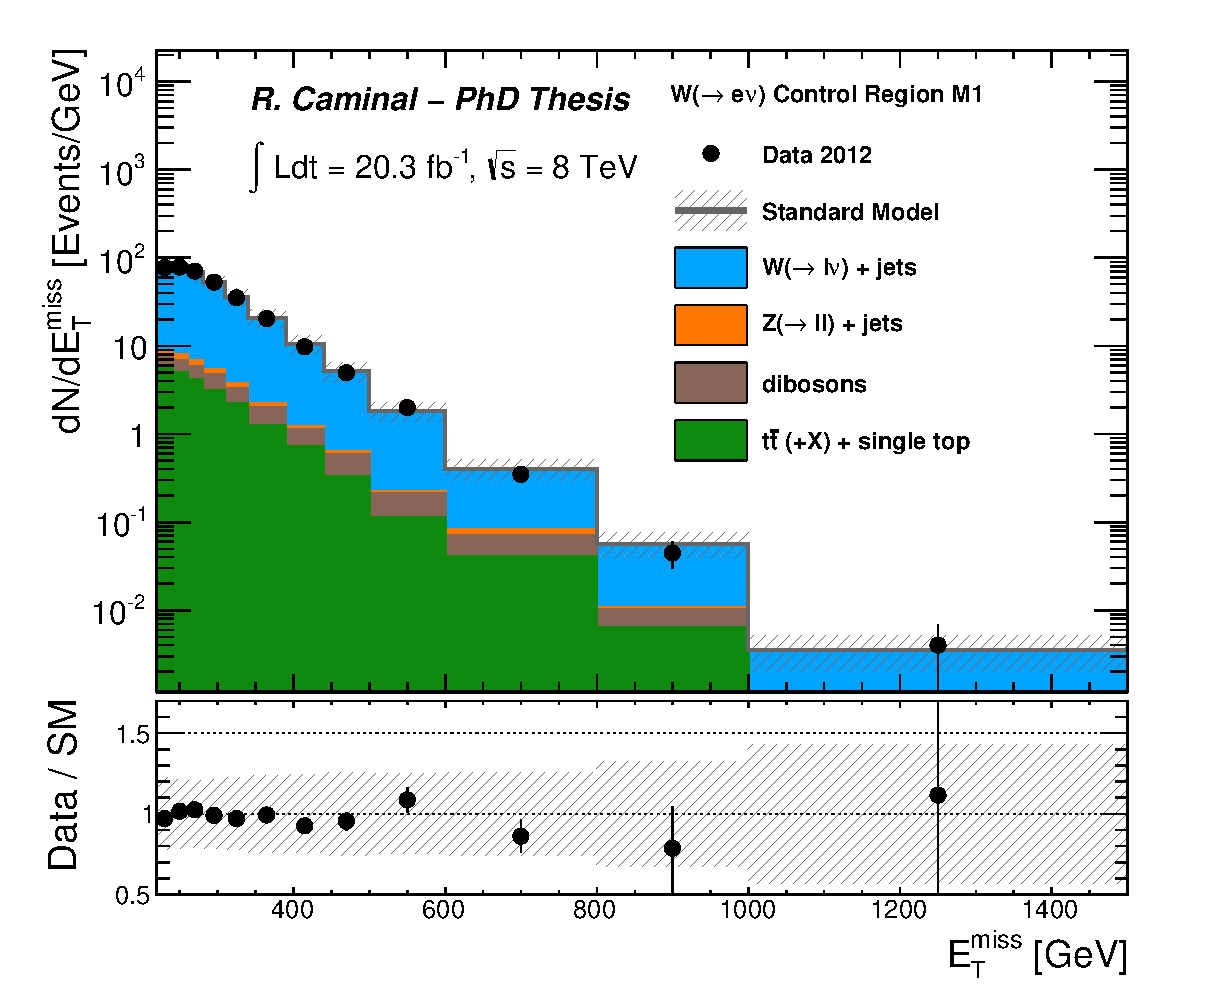
\includegraphics[width=0.495\textwidth]{MonojetAnalysis/Figures/plot_Stop_A6_CRele_met.eps}
      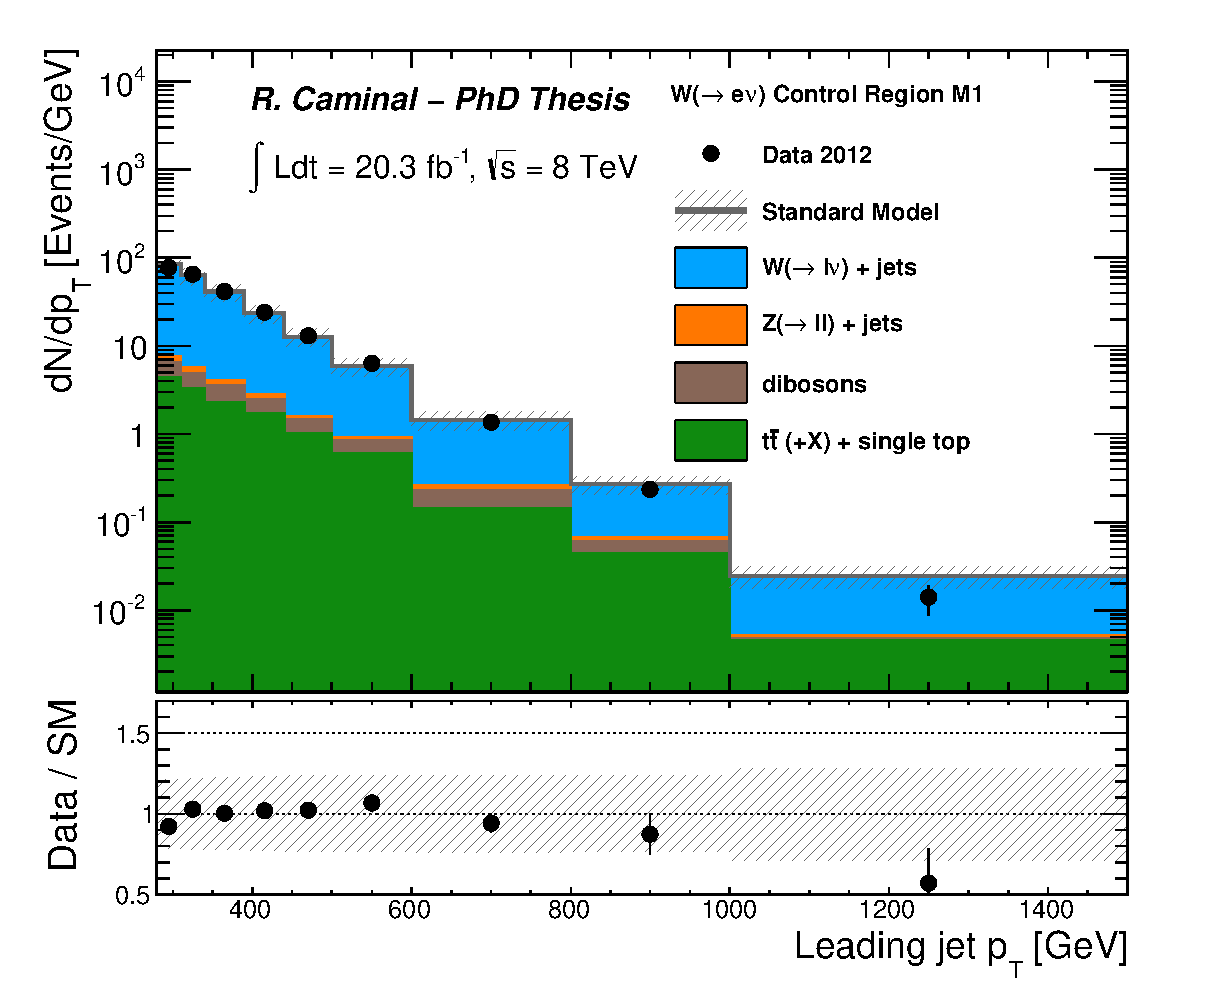
\includegraphics[width=0.495\textwidth]{MonojetAnalysis/Figures/plot_Stop_A6_CRele_pt1.eps}
    }
    \mbox{
      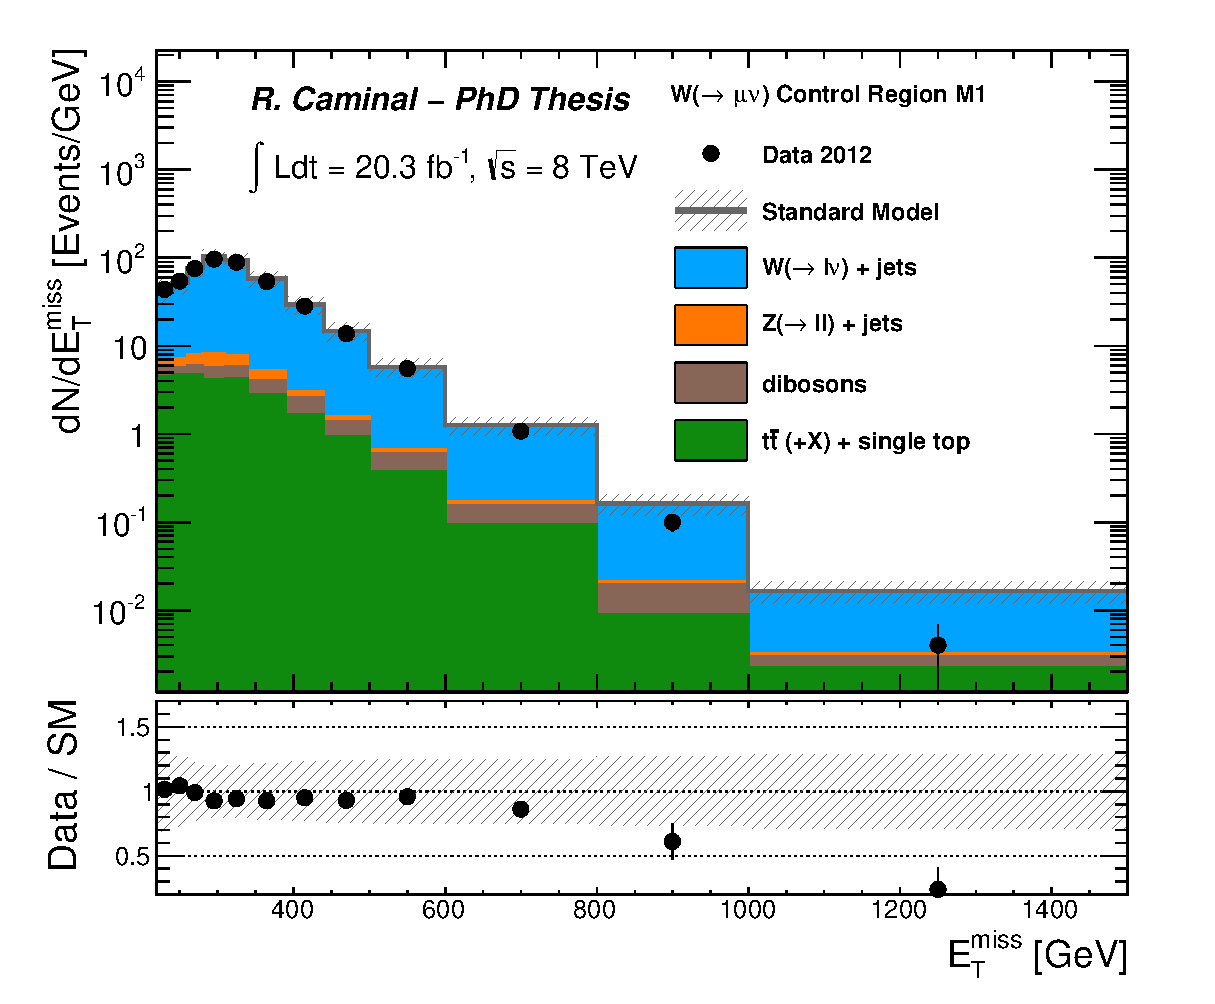
\includegraphics[width=0.495\textwidth]{MonojetAnalysis/Figures/plot_Stop_A6_CRwmn_met.eps}
      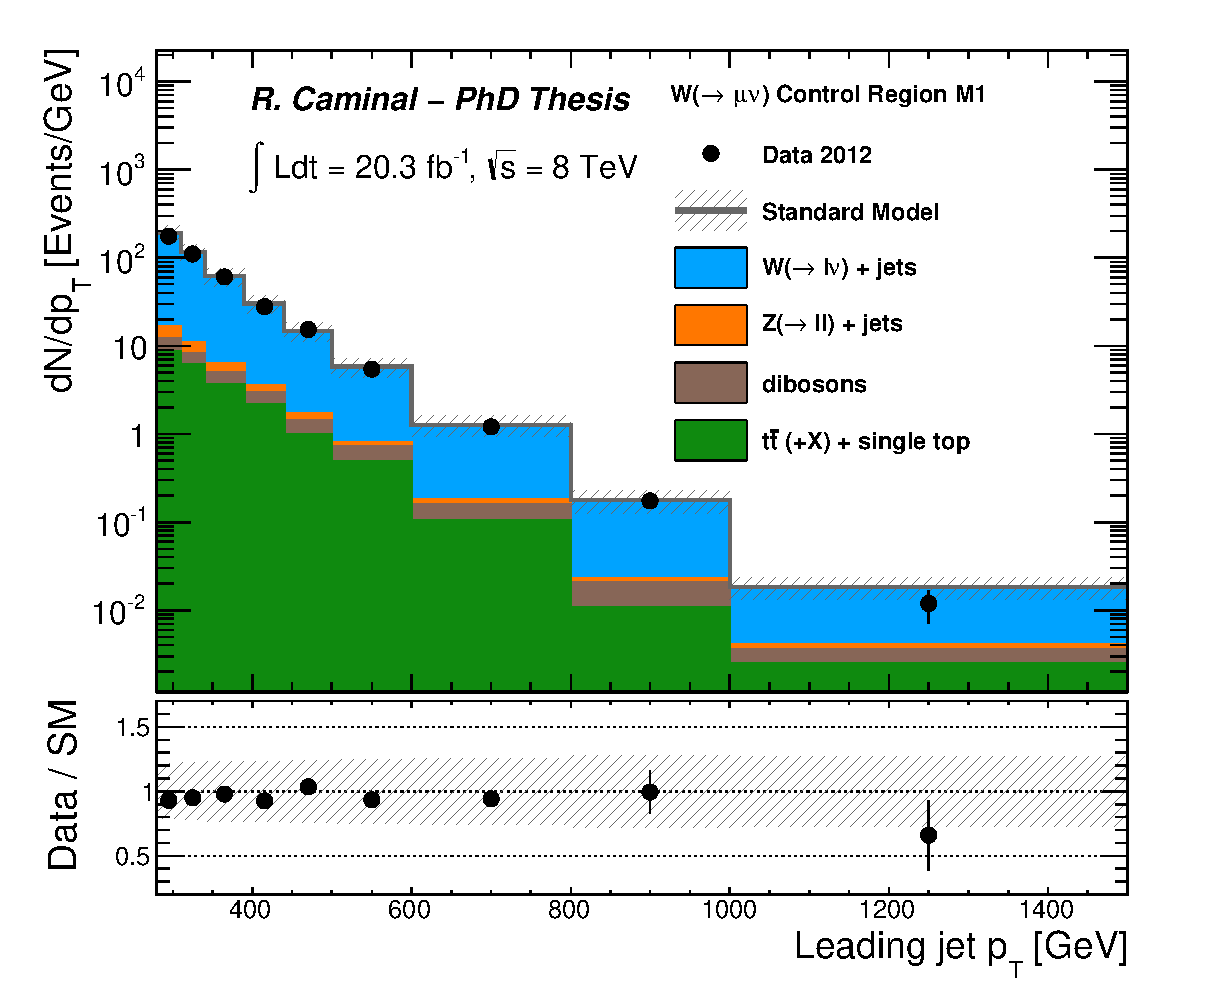
\includegraphics[width=0.495\textwidth]{MonojetAnalysis/Figures/plot_Stop_A6_CRwmn_pt1.eps}
    }
    \mbox{
      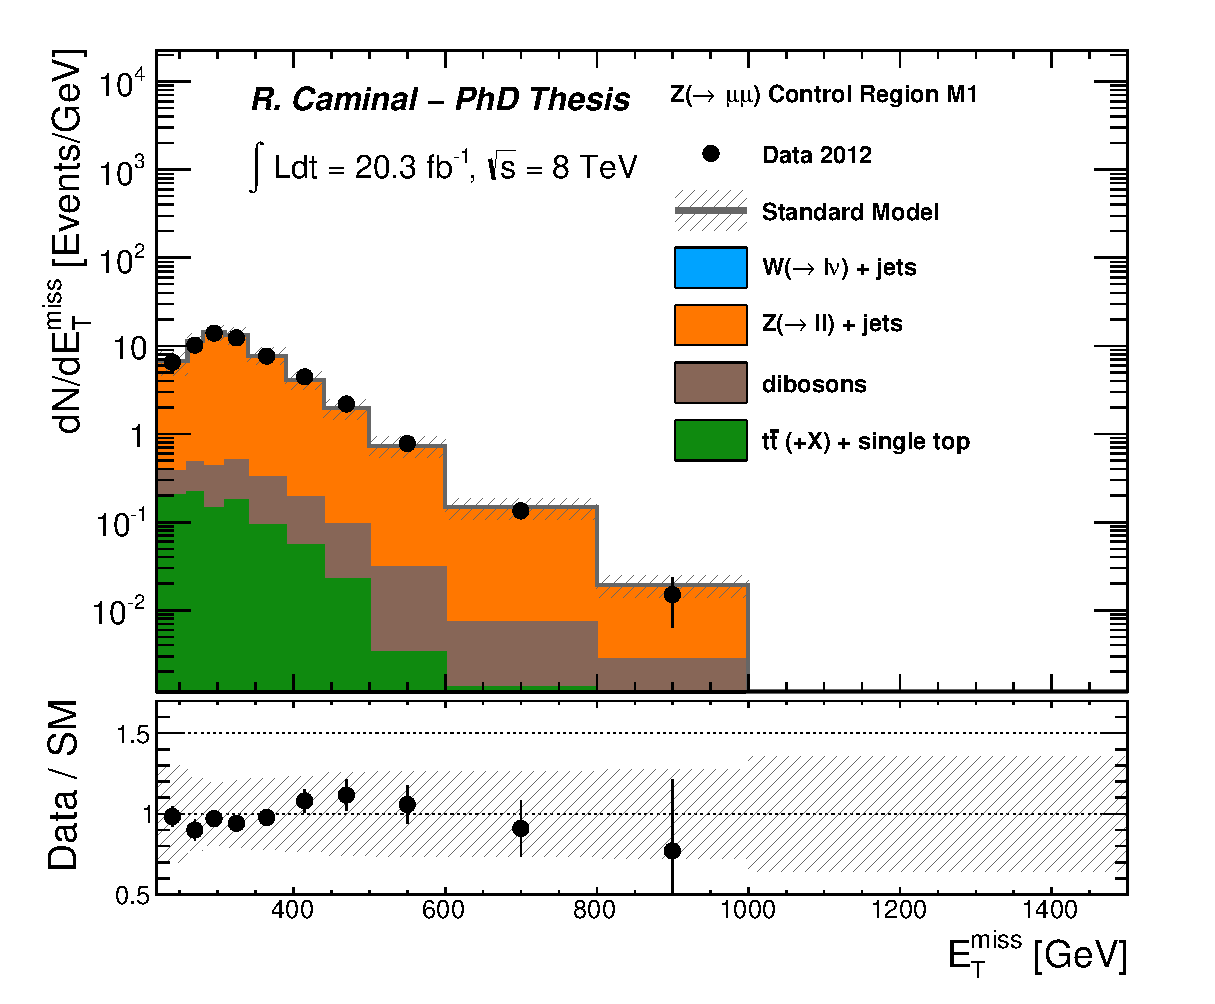
\includegraphics[width=0.495\textwidth]{MonojetAnalysis/Figures/plot_Stop_A6_CRzmm_met.eps}
      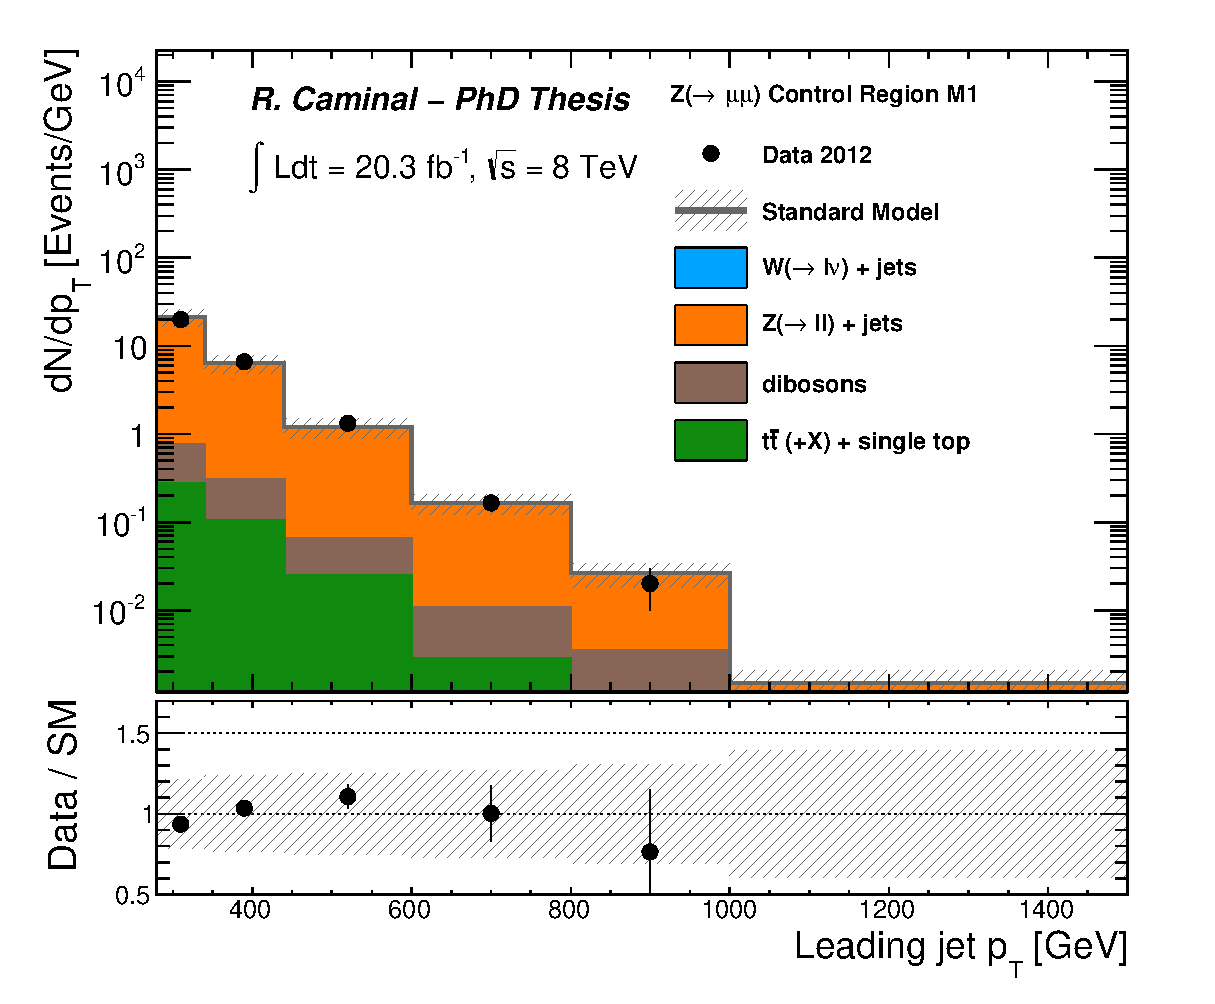
\includegraphics[width=0.495\textwidth]{MonojetAnalysis/Figures/plot_Stop_A6_CRzmm_pt1.eps}
    }
  \end{center}
  \caption[$\met$ and leading jet $\pt$ distributions in the three control region for the selection cuts of region M1 compared to the background predictions.]{$\met$ and leading jet $\pt$ distributions in the three control region for the selection cuts of region M1 compared to the background predictions. The error bands in the ratios include the statistical and experimental uncertainties on the background predictions.}
  \label{fig:Plot_M1_CR_beforeFit}
\end{figure}

Monte Carlo-based normalization factors, determined from the \sherpa{} simulation and including the boson $\pt$ re-weighting explained above, are defined for each of the signal selections to estimate the different electroweak background contributions in the signal regions.
As an illustrative example, the contribution from the dominant $\znn$ background process to a given signal region, $N^{Z(\rightarrow\nu\nu)}_{\text{signal}}$, would be determined using the $\wmn$+jets control sample in data, according to:

\begin{equation}
N^{Z(\rightarrow\nu\bar{\nu})}_{\text{signal}} = N^{\text{MC}(Z(\rightarrow\nu\bar{\nu}))}_{\text{signal}} \times
        \frac{\left(N^{\text{data}}_{W(\rightarrow\mu\nu),\text{control}} - N^{\text{non-}W}_{W(\rightarrow\mu\nu),\text{control}} \right)}{N^{\text{MC}}_{W(\rightarrow\mu\nu),\text{control}}},
\label{eq:scaleFactorZnunu}
\end{equation}

\noindent where $N^{\text{MC}(Z(\rightarrow\nu\bar{\nu}))}_{\text{signal}}$ is the background predicted by the MC simulation in the signal region, and $N^{\text{data}}_{W(\rightarrow\mu\nu),\text{control}}$, $N^{\text{MC}}_{W(\rightarrow\mu\nu),\text{control}}$, and $N^{\text{non-}W}_{W(\rightarrow\mu\nu),\text{control}}$ denote, in the control region, the number of $\wmn$+jets candidates in data and MC simulation, and the non-$\wmn$ background contribution, respectively.
The latest term refers mainly to top-quark and diboson processes, but also includes contributions from other $W/Z$+jets processes.
The normalization factor for this particular example (e.g. the last factor from the previous expression), is defined as the ratio of the number of observed $\wmn$+jets events over the total number of $\wmn$+jets simulated events, both in the control region.


\section{Fit of the background processes to the data}
    \label{sec:Fit}

The use of control samples to constrain the dominant background contribution from $\znn$ and $W$+jets, reduces significantly the otherwise relatively large theoretical and experimental systematic uncertainties, of the order of 20\%--30\%, associated with purely MC-based background predictions in the signal regions.
For each selection and in order to both normalize and constrain the corresponding background estimates in the different signal regions, and to determine the final uncertainty in the total background, the likelihood shown in Equation~\ref{eq:PdfFit},

\begin{equation}
L(\vec{\mu}, \vec{\alpha}) = 
 \prod_{c \in \text{regions}}{\frac{[\nu_c(\vec{\mu}, \vec{\alpha})]^{n_c}}{n_c!}e^{-\nu_c(\vec{\mu}, \vec{\alpha})}},
 \prod_{p\in\text{params}}{P_p(\alpha_p)},
\label{eq:PdfFit_copy}
\end{equation}

\noindent is simultaneously fitted to the $W(\rightarrow \mu\nu)$+jets, $\zmm$+jets and $W(\rightarrow e\nu)$+jets control samples, taking into account the cross contamination between the different background sources in the control samples.


\subsection{Normalization factors}
    \label{subsec:FreeParameters}

The likelihood includes unconstrained normalization factors that can adjust the relative contributions of the main processes ($\vec{\mu}$ in Equation \ref{eq:PdfFit_copy}).
In particular, three normalization factors are considered, determined from the $\wmn$+jets, $\zmm$+jets and $\wen$+jets control regions, denoted as \texttt{mu\_Wmn}, \texttt{mu\_Zmm} and \texttt{mu\_Ele}.
The \texttt{mu\_Wmn} factor is used to constrain the normalization of the $\wmn$+jets and the $\znn$ processes.
The \texttt{mu\_Zmm} factor sets the normalization of the $\zmm$+jets process.
Finally, the \texttt{mu\_Ele} factor determines the normalization of the $\wen$+jets, $\wtn$, $\zee$+jets and $\ztt$+jets processes.
Table~\ref{tab:scaleFactorsSummary} shows a summary of the normalization factors used to normalize each background process.

\begin{table}[!ht]
  \begin{center}
    \begin{small}
      \begin{tabular}{lc}
      \hline\hline
        {\bf Process} & {\bf Normalization factor} \\
        \hline
        $\wen$+jets   & \texttt{mu\_Ele} \\ 
        $\wmn$+jets   & \texttt{mu\_Wmn} \\ 
        $\wtn$   & \texttt{mu\_Ele} \\ 
        $\znn$   & \texttt{mu\_Wmn} \\ 
        $\zee$+jets   & \texttt{mu\_Ele} \\ 
        $\zmm$+jets   & \texttt{mu\_Zmm} \\ 
        $\ztt$+jets   & \texttt{mu\_Ele} \\ 
        Top      & -- \\ 
        Dibosons & -- \\ 
        Multijet & -- \\ 
       \hline\hline
      \end{tabular}
    \end{small}
  \end{center}
  \caption{Summary of the normalization factors used to normalize the different background processes in the signal region.}
  \label{tab:scaleFactorsSummary}
\end{table}

The choice for the normalization factor \texttt{mu\_Wmn} instead of \texttt{mu\_Zmm}, to estimate the $\znn$ contribution, is motivated by the statistical power of the $\wmn$ control sample in data, about seven times larger than the $\zmm$+jets control sample.
Appendix~\ref{app:ClosureTestZnunu} provides Monte Carlo studies, both at particle and at detector level, that confirm the validity of the use of \texttt{mu\_Wmn} to normalize the $\znn$ process.


\subsection{Systematic uncertainties}
    \label{subsec:MonojetSystematicUncertainties}

The likelihood from Eq.~\ref{eq:PdfFit_copy} also includes nuisance parameters, $\vec{\alpha}$, that parametrize the contributions of the processes as a function of variations in fractions of sigma, with respect to their nominal prediction, for each systematic uncertainty.
These nuisance parameters are normally distributed, with mean 0, indicating that they are centered in the value corresponding to the nominal prediction, and standard deviation 1, in units of potential systematic variations.
In the global fit, each nuisance parameter is initialized at such values, and the fit is then allowed to profile the different systematic uncertainties in order to find the configuration that maximizes the likelihood.
Values for the nuisance parameters largely differing from 0 would indicate a large mismodeling, and that the fit tries to accommodate to the data with an anomalously large variation of systematic uncertainties.

The systematic uncertainties considered in this analysis are summarized and related to their corresponding nuisance parameters in Table~\ref{tab:monosyslist}.
A description of each systematic source is detailed below.
For each uncertainty, the impact on the total background yield before the fit\footnote{Therefore, the effect in the background contribution corresponding to $\alpha_\text{syst} = \pm 1$} is also discussed.
These values are included as inputs in the global analysis fit.
The systematic uncertainties are assumed to be correlated through the different background processes, and control and signal regions, unless the contrary is stated.

%--- \ref{tab:monosyslist}
\begin{table}
\begin{center}
\begin{scriptsize}
\begin{tabular}{|l|l|}
\hline
\multicolumn{2}{|c|}{{\bf Parameter definition}} \\ \hline
{\bf Free parameters} & {\bf Definition}            \\
\hline
\texttt{mu\_Ele}             & Normalization factor \\ 
\texttt{mu\_Wmn}             & Normalization factor \\ 
\texttt{mu\_Zmm}             & Normalization factor \\ \hline \hline
{\bf Nuisance parameters} & {\bf Definition}           \\ 
\texttt{alpha\_JES   }       & Uncertainty on the jet energy scale. \\ 
\texttt{alpha\_JER   }       & Uncertainty on the Jet energy resolution. \\ 
\texttt{alpha\_JvfUnc}       & Uncertainty due to the jet vertex fraction cut. \\ 
\texttt{alpha\_Pileup}       & Uncertainty on the pileup reweighing. \\ 
\multirow{2}{*}{\texttt{alpha\_SCALEST}}      & Uncertainty on the cell out energy scale of the missing transverse \\
                    & energy. \\ 
\multirow{2}{*}{\texttt{alpha\_RESOST}}       & Uncertainty on the cell out energy resolution of the missing \\
                    & transverse energy. \\ 
\texttt{alpha\_EEFF  }       & Uncertainty on the identification efficiency of the electrons. \\ 
\texttt{alpha\_EGZEE }       & Uncertainty on the energy scale of the electrons (Z scale). \\ 
\texttt{alpha\_EGMAT }       & Uncertainty on the energy scale of the electrons (material). \\ 
\texttt{alpha\_EGLOW }       & Uncertainty on the energy scale of the electrons (low momentum). \\ 
\texttt{alpha\_EGPS  }       & Uncertainty on the energy scale of the electrons (presampler). \\ 
\texttt{alpha\_EGRES }       & Uncertainty on the energy resolution of the electrons. \\ 
\texttt{alpha\_MEFF  }       & Uncertainty on the identification efficiency of the muons.\\ 
\texttt{alpha\_MSCALE}       & Uncertainty on the energy scale of the muons. \\ 
\multirow{2}{*}{\texttt{alpha\_MMS}}          & Uncertainty on the energy resolution of the muons (muon \\
                    & spectrometer). \\ 
\texttt{alpha\_MID         } & Uncertainty on the energy resolution of the muons (inner detector) \\ 
\texttt{alpha\_ktfac       } & Uncertainty on the factorization scale of the W/Z+jets. \\ 
\texttt{alpha\_qfac        } & Uncertainty on the matching scale of the W/Z+jets. \\ 
\texttt{alpha\_pdfUnc      } & Uncertainty on the PDFs of the $W/Z$+jets processes. \\ 
\multirow{2}{*}{\texttt{alpha\_bosonPtReweight}}& Uncertainty on the re-weighting of the $W/Z$+jets Sherpa samples, \\
                    & based on the truth boson $p_T$. \\ 
\multirow{3}{*}{\texttt{alpha\_WZtransfer}}   & Uncertainty on the $\znn$ estimation to cover for the \\
                    & differences on the MC modeling and EWK NLO corrections \\
                    & between $W$ and $Z$ processes. \\
\texttt{alpha\_ttbarGen    } & Uncertainty on the MC generator of the ttbar sample. \\ 
\texttt{alpha\_ttbarXsec   } & Uncertainty on the cross-section of the ttbar sample. \\ 
\texttt{alpha\_ttbarRad    } & Uncertainty on the ISR/FSR of the ttbar sample. \\ 
\texttt{alpha\_ttbarRen    } & Uncertainty on the renormalization scale of the ttbar sample. \\ 
\texttt{alpha\_ttbarFac    } & Uncertainty on the factorization scale of the ttbar sample. \\ 
\texttt{alpha\_ttbarPs     } & Uncertainty on the parton shower modelling of the ttbar sample. \\ 
\texttt{alpha\_singleTGen  } & Uncertainty on the MC generator of the single top sample. \\ 
\texttt{alpha\_singleTXsecS} & Uncertainty on the $s$-channel cross-section of the single top sample. \\ 
\texttt{alpha\_singleTXsecT} & Uncertainty on the $t$-channel cross-section of the single top sample. \\ 
\texttt{alpha\_singleTXsecW} & Uncertainty on the $Wt$ cross-section of the single top sample. \\ 
\texttt{alpha\_singleTRad  } & Uncertainty on the ISR/FSR of the single top sample. \\ 
\texttt{alpha\_singleTInt  } & Uncertainty on the interference with ttbar of the single top sample. \\ 
\multirow{2}{*}{\texttt{alpha\_singleTPs}}    & Uncertainty on the parton shower modelling for the $Wt$ channel \\
                    & of the single top sample. \\ 
\texttt{alpha\_dibRen      } & Uncertainty on the renormalization scale of the diboson sample.  \\ 
\texttt{alpha\_dibMatch    } & Uncertainty on the matching scale of the diboson sample. \\ 
\texttt{alpha\_dibFac      } & Uncertainty on the factorization scale of the diboson sample.  \\ 
\texttt{alpha\_dibXsec     } & Uncertainty on the cross-section of the diboson sample. \\ 
\multirow{2}{*}{\texttt{alpha\_qcdNorm}}      & Uncertainty on the normalization of the multi jet background \\
                    & estimation. \\
\texttt{alpha\_Luminosity  } & Uncertainty on the measurement of the luminosity in ATLAS. \\ \hline
\end{tabular}
\end{scriptsize}
\end{center}
\caption{List of all nuisance parameters used in the analysis and their definition in terms of
normalization factors and sources of systematic uncertainty.}
\label{tab:monosyslist}
\end{table} 


\paragraph{Jet Energy Scale:} The uncertainty on the absolute jet energy scale (JES) is one of the main uncertainties.
In the analysis it is parametrized by a single nuisance parameter, although is the result of combining 18 systematic sources\footnote{The performance of the fit has also been checked when 18 nuisance parameters are considered, and has lead to identical results.}, from the different steps of the jet energy scale calibration.
The effect of this uncertainty on the total MC prediction, before it is profiled in the global fit.
Before the fit it is approximately 7\% in both the signal and control regions.

\paragraph{Jet Energy Resolution:} The effect of the jet energy resolution (JER) in the total background yield is measured in each of the signal regions, and found to be less than 1\%.

\paragraph{Jet Vertex Fraction:} The effect of a possible mismodeling in the JVF distribution is investigated by studying the impact in the background yields when the requirement is varied from 0.5 to 0.47 and 0.53.
An effect below 1\% in the total background yield is found in all the signal regions.

\paragraph{Pile up:} The MC generated events need to be re-weighted in order to correctly describe the pileup conditions in the collisions.
This weights are extracted from the comparison of the number of interactions per bunch crossing distribution in both data and MC simulation.
Variations on these weights lead to negligible effects in the total background prediction.

\paragraph{$\met$ cell-out:}The resolution and scale uncertainties of the CellOut term of the $\met$ are also considered, and each of them is parametrized by a single nuisance parameter.
The effect of these uncertainties to the total background in the different signal regions is less than 1\%.

\paragraph{Leptons:} The uncertainty on the electron identification varies the total background yield in the signal regions by less than 1\%, and is parametrized by a single nuisance parameter.
The effect of the electron energy resolution, also parametrized by one nuisance parameter, leads to a negligible effect.
The uncertainty on the electron energy scale accounts for: the variations coming from the $Z$~scale uncertainty; the modeling of the interaction of the electrons with the calorimeter; the presampler scale uncertainty; and the scale uncertainty for low-$\pt$ electrons.
This is included in the fit via four separated nuisance parameters, which altogether introduce less than a 0.5\% variation in the total background yield.

The uncertainty on the muon identification translates into a 1\% variation on the total background in all the signal regions, and is parametrized by one nuisance parameter.
The uncertainty on the muon energy resolution accounts for the resolution effects coming from the Inner Detector and the Muon Spectrometer.
This uncertainty, parametrized with two different nuisance parameters, has a negligible effect on the total background contribution.
Finally, the uncertainty on the muon energy scale, affects the total background prediction in the signal regions by approximately 0.5\%, and is introduced in the global fit via one nuisance parameter.

\paragraph{Theoretical uncertainties on the $W/Z$+jets processes:}
Uncertainties on the factorization, renormalization, and parton-shower matching scales and PDFs of the $W/Z$+jets processes, are parametrized, each of them, by a different nuisance parameter.
Combined, they produce a variation between 20\% and 25\% in the total background yields, in the different signal selections.
An additional nuisance parameter is devoted to parametrize the uncertainty of the re-weighting of the boson $\pt$, and affects the total background prediction by a 2\%.
Finally, systematic uncertainties to account for the validity of the use of the $\wmn$+jets process to extract the normalization for $\znn$ and higher-order electroweak corrections affecting differently the $W$+jets and the $Z$+jets processes, are also considered~\cite{Denner:2009gj,Denner:2011vu,Denner:2012ts}.
These two effects are parametrized together by a single nuisance parameter, and modify the total background yield between 2\% and 4\% in the different signal regions.
More details on the estimation of this uncertainty can be found in Appendix~\ref{app:ClosureTestZnunu}.

\paragraph{Theoretical uncertainties on the top-quark-related processes:} Uncertainties on the absolute $\ttbar$ and single top cross sections; uncertainties on the MC generators and the modeling of parton showers employed; variations in the set of parameters that govern the parton showers and the amount of initial- and final-state soft gluon radiation; and uncertainties due to the choice of renormalization and factorization scales and PDFs are considered.
The effect of these systematic uncertainties on the total background prediction, varies between 1.6\% and 1.0\% for the different signal selections, and are represented by 13 different nuisance parameters in the fit.

\paragraph{Theoretical uncertainties on the diboson:} These uncertainties are estimated in a similar way as for the top-quark-related processes, and translate to an effect on the total background between 0.7\% and 2.3\%.
In the fit, these uncertainties are parametrized by 4 nuisance parameters.

\paragraph{Multijet uncertainty:} The systematic uncertainty on the multijet is computed by comparing the predictions when using different response functions.
A 100\% variation in the multijet prediction is observed, leading to a 1\% uncertainty on the total background for the M1 selection.

\paragraph{Luminosity:} The uncertainty on the determination of the total integrated luminosity introduces an 2.8\% variation in the total background yield.
This systematic uncertainty is parametrized with a single nuisance parameter in the fit.

\paragraph{Statistical uncertainty in the MC simulations:} 
In order to avoid fluctuations in the global fit, the statistical uncertainties on the Monte Carlo simulations are only considered if they are larger than 5\%.
This limitation has a negligible impact on the results, but contributes to a more robust performance of the fit.

\paragraph{Trigger efficiency:} All the systematic effects related to the trigger efficiency have a negligible impact on the analysis.

\paragraph{}


\section{Estimation of the background contributions}
    \label{sec:ControlRegions}

The data and background predictions for the M1 to M6 selections in the $\wen$+jets, $\wmn$+jets and $\zmm$+jets control regions are presented in Tables~\ref{tab:ControlRegion_CRele}, \ref{tab:ControlRegion_CRwmn} and \ref{tab:ControlRegion_CRzmm}, respectively.
In each of the kinematic selections, the MC predicted yields before and after the global fit are shown.
The normalization factors for the background processes in the different selections are extracted from these tables, and are shown in Table~\ref{tab:scaleFactors}.
The uncertainties on the normalization factors include both the statistical and systematic components.
The fitted values for the nuisance parameters as well as the correlations among the normalization factors and the nuisance parameters in the global fit, are presented in Appendix~\ref{app:FitResults}, for all the analysis selections.

The normalizations are compatible with 1 within uncertainties in all the selections, except in M5 and M6.
In these regions, the boson $\pt$ distributions can not be effectively corrected, since a single weight is used for those events with boson $\pt>\unit[400]{GeV}$.
Therefore, the boson $\pt$ re-weighting does not modify the shape of this distribution, but only introduces a variation in the normalization of the $W/Z$+jets samples, that needs to be compensated by the normalization factors from the fit.

\begin{table}[!ht]
\begin{center}
\begin{small}
\begin{tabular*}{\textwidth}{@{\extracolsep{\fill}}lrrr}\hline
{\bf Control Region} $\wen$  & \textbf{M1} & \textbf{M2} & \textbf{M3}  \\
    Observed events  (20.3 fb${}^{-1}$)& $9271$                &  $1835$                       & $417$           \\ \hline
                                                                                                               
    SM prediction (post-fit)&                      $9270 \pm 110$        &  $1840 \pm 45$                & $420 \pm 20$  \\ \hline
                                                                                                               
    $\wen$+jets &                      $6580 \pm 130$        &  $1260 \pm 43$                & $270 \pm 17$  \\
                                                                                                               
    $\wmn$+jets &                      $39 \pm 5$            &  $10 \pm 2$                   & $2.2 \pm 0.4$  \\
                                                                                                               
    $\wtn$        &                      $1640 \pm 40$         &  $350 \pm 13$                 & $84 \pm 6$     \\
                                                                                                               
    $\zee$+jets       &                      $0.04_{-0.04}^{+0.07}$&  $0.03_{-0.03}^{+0.05}$       & $-$            \\
                                                                                                               
    $\zmm$+jets       &                      $3.6 \pm 0.5$         &  $1.2 \pm 0.2$                & $0.7 \pm 0.1$   \\
                                                                                                               
    $\ztt$+jets        &                      $116 \pm 3$           &  $17 \pm 1$                   & $4.7 \pm 0.4$   \\
                                                                                                               
    $\znn$        &                      $17 \pm 3$            &  $4.6 \pm 0.7$                & $1.2 \pm 0.2$   \\
                                                                                                               
    $\ttbar$, single top &               $600 \pm 80$          &  $120 \pm 20$                 & $31 \pm 5$    \\
                                                                                                               
    Dibosons      &                      $280 \pm 90$          &  $80 \pm 30$                  & $22 \pm 8$   \\  \hline

    SM prediction (pre-fit)                 & $9354$  & $1873$ & $416$ \\                      
    \hline                                                 
                                                                 
    Fit input $\wen$+jets                  & $6644$  & $1287$ & $271$ \\
    %%                                                           
    Fit input $\wmn$+jets                  & $41$    & $11$   & $2.4$ \\
    %%                                                           
    Fit input $\wtn$                  & $1650$  & $352$  & $83$  \\
    %%                                                           
    Fit input $\zee$+jets                  & $0.04$  & $0.04$ & $-$   \\
    %%                                                           
    Fit input $\zmm$+jets                  & $3.7$   & $1.2$  & $0.7$ \\
    %%                                                           
    Fit input $\ztt$+jets                  & $117$   & $17$   & $4.6$ \\
    %%                                                           
    Fit input $\znn$                  & $18$    & $4.9$  & $1.3$ \\
    %%                                                           
    Fit input $\ttbar$, single top    & $600$   & $120$  & $31$  \\
    %%                                                           
    Fit input dibosons                & $280$   & $80$   & $22$  \\

    
    \hline \hline
                 & & & \\                                                          
    \hline 
                                                                         
{\bf  Control Region} $\wen$  & \textbf{M4} & \textbf{M5} & \textbf{M6}  \\
    Observed events  (20.3 fb${}^{-1}$)& $934$                 & $120$        &  $61$             \\ \hline
                                                                                                
    SM prediction (post-fit)                     & $934 \pm 31$          & $120 \pm 11$ &  $61 \pm 8$     \\ \hline
                                                                                                
    $\wen$+jets                             & $625 \pm 29$          & $72 \pm 8$   &  $34 \pm 6$     \\
                                                                                                
    $\wmn$+jets                             & $4.6 \pm 0.7$         & $0.8 \pm 0.2$&  $0.4 \pm 0.2$  \\
                                                                                                
    $\wtn$                             & $168 \pm 8$           & $25 \pm 3$   &  $11 \pm 2$     \\
                                                                                                
    $\zee$+jets                             & $0.03_{-0.03}^{+0.05}$& $-$         &  $-$           \\
                                                                                                
    $\zmm$+jets                             & $1.1 \pm 0.2$         & $0.5 \pm 0.1$&  $0.4 \pm 0.1$  \\
                                                                                                
    $\ztt$+jets                             & $10.4 \pm 0.6$        & $2.3 \pm 0.4$&  $1.5 \pm 0.5$  \\
                                                                                                
    $\znn$                             & $2.2 \pm 0.4$         & $0.4 \pm 0.1$&  $0.28 \pm 0.06$\\
                                                                                                
    $\ttbar$, single top               & $79 \pm 11$           & $11 \pm 2$   &  $8 \pm 2$      \\
                                                                                                
    Dibosons                           & $44 \pm 17$           & $9 \pm 3$    &  $5 \pm 2$      \\

    \hline

    SM prediction (pre-fit)                 & $947$  & $126$  & $74$  \\                      
    \hline                                                      
                                                                        
    Fit input $\wen$+jets                  & $634$  & $75$   & $43$  \\
    %%                                                                   
    Fit input $\wmn$+jets                  & $4.7$    & $1.0$    & $0.5$   \\
    %%                                                                   
    Fit input $\wtn$                  & $171$  & $26$   & $14$  \\
    %%                                                                   
    Fit input $\zee$+jets                  & $0.04$    & $-$    & $-$   \\
    %%                                                                   
    Fit input $\zmm$+jets                  & $1.0$    & $0.6$    & $0.6$   \\
    %%                                                                   
    Fit input $\ztt$+jets                  & $10.6$   & $2.4$    & $1.9$   \\
    %%                                                                   
    Fit input $\znn$                  & $2.3$    & $0.5$    & $0.37$   \\
    %%                                                                   
    Fit input $\ttbar$, single top    & $79$   & $11$   & $8$   \\
    %%                                                                   
    Fit input dibosons                & $44$   & $9$    & $5$   \\

    \hline \hline

    \end{tabular*}
    \end{small}

    \end{center}
    \caption[Data and SM background predictions in the $\wen$+jets control regions M1 to M6.]
{Data and SM background predictions in the $\wen$+jets control regions M1 to M6. 
      For the SM predictions both statistical and systematic uncertainties are included.
        Note that in each case the individual 
        uncertainties can be correlated, and do not necessarily add up quadratically to the total background uncertainty.
    }
\label{tab:ControlRegion_CRele}
\end{table}
 %--- \ref{tab:ControlRegion_CRele}
\begin{table}[!ht]
\begin{center}
\begin{small}
\begin{tabular*}{\textwidth}{@{\extracolsep{\fill}}lrrr}\hline
{\bf Control Region} $\wmn$  & \textbf{M1} & \textbf{M2} & \textbf{M3}  \\
    Observed events  (20.3 fb${}^{-1}$)&  $14786$                   & $4285$        & $946$            \\ \hline
                                                                                                     
    SM prediction (post-fit)                     &  $14780 \pm 150$           & $4280 \pm 70$ & $950 \pm 30$     \\ \hline
                                                                                                     
    $\wen$+jets                             &  $0.4 \pm 0.2$             & $-$           & $-$              \\
                                                                                                     
    $\wmn$+jets                             &  $12110 \pm 200$           & $3500 \pm 90$ & $750 \pm 37$      \\
                                                                                                     
    $\wtn$                             &  $1130 \pm 30$             & $330 \pm 15$  & $79 \pm 6$       \\
                                                                                                     
    $\zee$+jets                             &  $-$                      & $-$           & $-$              \\
                                                                                                     
    $\zmm$+jets                             &  $290 \pm 20$              & $71 \pm 4$    & $13 \pm 1$     \\
                                                                                                     
    $\ztt$+jets                             &  $43 \pm 3$                & $8.5 \pm 0.6$ & $1.8 \pm 0.3$  \\
                                                                                                     
    $\znn$                             &  $4.2 \pm 0.4$             & $0.8 \pm 0.1$ & $0.08 \pm 0.02$  \\
                                                                                                     
    $\ttbar$, single top               &  $880 \pm 90$              & $240 \pm 35$  & $65 \pm 10$    \\
                                                                                                     
    Dibosons                           &  $330 \pm 110$             & $130 \pm 53$  & $40 \pm 17$      \\ \hline

    SM prediction (pre-fit)            &  $15531$  & $4513$ & $1023$ \\                      
    \hline                                                   
                                                                    
    Fit input $\wen$+jets                  &  $0.4$    & $-$    & $-$    \\
    %%                                                              
    Fit input $\wmn$+jets                  &  $12839$  & $3725$ & $824$  \\
    %%                                                              
    Fit input $\wtn$                  &  $1142$   & $342$  & $79$   \\
    %%                                                              
    Fit input $\zee$+jets                  &  $-$      & $-$    & $-$    \\
    %%                                                              
    Fit input $\zmm$+jets                  &  $291$    & $67$   & $13$   \\
    %%                                                              
    Fit input $\ztt$+jets                  &  $44$     & $8.7$  & $1.8$  \\
    %%                                                              
    Fit input $\znn$                  &  $4.5$    & $0.8$  & $0.10$ \\
    %%                                                              
    Fit input $\ttbar$, single top    &  $880$    & $240$  & $65$   \\
    %%                                                              
    Fit input dibosons                &  $330$    & $130$  & $40$   \\

    
    \hline \hline
                 & & & \\                                                          
    \hline 


{\bf Control Region} $\wmn$  & \textbf{M4} & \textbf{M5} & \textbf{M6}  \\
    Observed events  (20.3 fb${}^{-1}$)& $1271$         & $267$          &  $147$           \\ \hline
                                                                                           
    SM prediction (post-fit)                     & $1271 \pm 36$  & $267 \pm 16$   &  $147 \pm 12$   \\ \hline
                                                                                           
    $\wen$+jets                             & $-$           & $-$           &  $-$           \\
                                                                                           
    $\wmn$+jets                             & $1004 \pm 43$  & $201 \pm 18$   &  $109 \pm 13$   \\
                                                                                           
    $\wtn$                             & $99 \pm 5$     & $23 \pm 3$     &  $11 \pm 2$     \\
                                                                                           
    $\zee$+jets                             & $-$           & $-$           &  $-$           \\
                                                                                           
    $\zmm$+jets                             & $21 \pm 2$     & $2.4 \pm 0.5$  &  $1.4 \pm 0.4$  \\
                                                                                           
    $\ztt$+jets                             & $2.6 \pm 0.3$  & $0.6 \pm 0.1$  &  $0.4 \pm 0.1$  \\
                                                                                           
    $\znn$                             & $0.14 \pm 0.02$& $0.05 \pm 0.01$&  $0.03 \pm 0.01$\\
                                                                                           
    $\ttbar$, single top               & $98 \pm 15$    & $25 \pm 4$     &  $15 \pm 2$     \\
                                                                                           
    Dibosons                           & $47 \pm 21$    & $14 \pm 6$     &  $10 \pm 5$     \\

    \hline

    SM prediction (pre-fit)                 & $1310$  & $316$ & $185$ \\                      
    \hline                                                               
                                                                         
    Fit input $\wen$+jets                  & $-$     & $-$   & $-$   \\
    %%                                                                   
    Fit input $\wmn$+jets                  & $1043$  & $249$ & $144$ \\
    %%                                                                   
    Fit input $\wtn$                  & $100$   & $25$  & $14$  \\
    %%                                                                   
    Fit input $\zee$+jets                  & $-$     & $-$   & $-$   \\
    %%                                                                   
    Fit input $\zmm$+jets                  & $19$    & $3.5$   & $2.0$   \\
    %%                                                                   
    Fit input $\ztt$+jets                  & $2.6$     & $0.6$   & $0.4$   \\
    %%                                                                   
    Fit input $\znn$                  & $0.15$     & $0.06$   & $0.04$   \\
    %%                                                                   
    Fit input $\ttbar$, single top    & $98$    & $25$  & $15$  \\
    %%                                                                   
    Fit input dibosons                & $47$    & $14$  & $10$  \\

    \hline \hline

    \end{tabular*}
    \end{small}

    \end{center}
    \caption[Data and SM background predictions in the $\wmn$+jets control regions M1 to M6.]
{Data and SM background predictions in the $\wmn$+jets control regions M1 to M6. 
      For the SM predictions both statistical and systematic uncertainties are included.
        Note that in each case the individual 
        uncertainties can be correlated, and do not necessarily add up quadratically to the total background uncertainty.
    }
\label{tab:ControlRegion_CRwmn}
\end{table}
 %--- \ref{tab:ControlRegion_CRwmn}
\begin{table}[!ht]
\begin{center}
\begin{small}
\begin{tabular*}{\textwidth}{@{\extracolsep{\fill}}lrrr}\hline
{\bf Control Region} $\zmm$  & \textbf{M1} & \textbf{M2} & \textbf{M3}  \\
    Observed events  (20.3 fb${}^{-1}$)& $2100$        & $650$          & $131$            \\ \hline
                                                                                         
    SM prediction (post-fit)                     & $2100 \pm 50$ & $650 \pm 26$   & $130 \pm 12$     \\ \hline
                                                                                         
    $\wen$+jets                             & $-$           & $-$            & $-$              \\
                                                                                         
    $\wmn$+jets                             & $2.4 \pm 0.2$ & $0.8 \pm 0.2$  & $0.3 \pm 0.1$     \\
                                                                                         
    $\wtn$                             & $0.6 \pm 0.1$ & $0.28 \pm 0.03$& $0.02 \pm 0.01$  \\
                                                                                         
    $\zee$+jets                             & $-$           & $-$            & $-$              \\
                                                                                         
    $\zmm$+jets                             & $2010 \pm 50$ & $620 \pm 27$   & $120 \pm 12$   \\
                                                                                         
    $\ztt$+jets                             & $2.9 \pm 0.3$ & $1.0 \pm 0.1$  & $0.28 \pm 0.03$\\
                                                                                         
    $\znn$                             & $-$           & $-$            & $-$              \\
                                                                                         
    $\ttbar$, single top               & $32 \pm 9$    & $8 \pm 2$      & $1 \pm 1$      \\
                                                                                         
    Dibosons                           & $58 \pm 21$   & $21 \pm 7$     & $5 \pm 3$        \\ \hline

    SM prediction (pre-fit)                & $2140$  & $621$  & $132$   \\                      
    \hline                                                         
                                                                   
    Fit input $\wen$+jets                  & $-$     & $-$    & $-$     \\
    %%                                                             
    Fit input $\wmn$+jets                  & $2.5$   & $0.8$  & $0.3$   \\
    %%                                                             
    Fit input $\wtn$                  & $0.6$   & $0.3$  & $0.02$  \\
    %%                                                             
    Fit input $\zee$+jets                  & $-$     & $-$    & $-$     \\
    %%                                                             
    Fit input $\zmm$+jets                  & $2044$  & $590$  & $125$   \\
    %%                                                             
    Fit input $\ztt$+jets                  & $3.0$   & $1.0$  & $0.3$   \\
    %%                                                             
    Fit input $\znn$                  & $-$     & $-$    & $-$     \\
    %%                                                             
    Fit input $\ttbar$, single top    & $32$    & $8$    & $1$     \\
    %%                                                             
    Fit input dibosons                & $58$    & $21$   & $5$     \\

    
    \hline \hline
                 & & & \\                                                          
    \hline 


{\bf Control Region} $\zmm$  & \textbf{M4} & \textbf{M5} & \textbf{M6}  \\
    Observed events  (20.3 fb${}^{-1}$)& $186$          & $27$           &  $15$            \\ \hline
                                                                                           
    SM prediction (post-fit)                     & $186 \pm 14$   & $27 \pm 5$     &  $15 \pm 4$     \\ \hline
                                                                                           
    $\wen$+jets                             & $-$           & $-$           &  $-$           \\
                                                                                           
    $\wmn$+jets                             & $0.31 \pm 0.08$& $0.13 \pm 0.02$&  $0.05 \pm 0.01$\\
                                                                                           
    $\wtn$                             & $0.02 \pm 0.00$& $0.02 \pm 0.01$&  $-$           \\
                                                                                           
    $\zee$+jets                             & $-$           & $-$           &  $-$           \\
                                                                                           
    $\zmm$+jets                             & $176 \pm 14$   & $25 \pm 5$     &  $14 \pm 4$     \\
                                                                                           
    $\ztt$+jets                             & $0.28 \pm 0.03$& $0.10 \pm 0.03$&  $0.05 \pm 0.01$\\
                                                                                           
    $\znn$                             & $-$           & $-$           &  $-$           \\
                                                                                           
    $\ttbar$, single top               & $3 \pm 2$      & $0.2 \pm 0.2$  &  $0.2 \pm 0.2$  \\
                                                                                           
    Dibosons                           & $7 \pm 3$      & $1.1 \pm 0.6$  &  $0.7 \pm 0.3$  \\

    \hline

    SM prediction (pre-fit)                 & $173$  & $38$  & $22$  \\                      
    \hline                                                              
                                                                        
    Fit input $\wen$+jets                  & $-$    & $-$   & $-$   \\
    %%                                                                  
    Fit input $\wmn$+jets                  & $0.33$    & $0.16$   & $0.07$   \\
    %%                                                                  
    Fit input $\wtn$                  & $0.02$    & $0.02$   & $0.00$   \\
    %%                                                                  
    Fit input $\zee$+jets                  & $-$    & $-$   & $-$   \\
    %%                                                                  
    Fit input $\zmm$+jets                  & $163$  & $37$  & $21$  \\
    %%                                                                  
    Fit input $\ztt$+jets                  & $0.28$    & $0.11$   & $0.06$   \\
    %%                                                                  
    Fit input $\znn$                  & $-$    & $0.00$   & $0.00$   \\
    %%                                                                  
    Fit input $\ttbar$, single top    & $3$    & $0.2$   & $0.2$   \\
    %%                                                                  
    Fit input dibosons                & $7$    & $1.1$   & $0.7$   \\

    \hline \hline

    \end{tabular*}
    \end{small}

    \end{center}
    \caption[Data and SM background predictions in the $\zmm$+jets control regions M1 to M6.]
{Data and SM background predictions in the $\zmm$+jets control regions M1 to M6. 
      For the SM predictions both statistical and systematic uncertainties are included.
        Note that in each case the individual 
        uncertainties can be correlated, and do not necessarily add up quadratically to the total background uncertainty.
    }
\label{tab:ControlRegion_CRzmm}
\end{table}
 %--- \ref{tab:ControlRegion_CRzmm}

\begin{table}[tb]
\begin{center}
\begin{small}
\renewcommand{\baselinestretch}{1.2}
\begin{tabular*}{\textwidth}{@{\extracolsep{\fill}}cccc}\hline
\hline
\multicolumn{4}{c} {\bf Normalization factors} \\ 
\hline
{\bf Selection} & \texttt{mu\_Ele} &  \texttt{mu\_Wmn} & \texttt{mu\_Zmm} \\ 
\hline
M1              & $0.99 \pm 0.21$  & $0.94 \pm 0.20$   & $0.98 \pm 0.20$ \\ 
M2              & $0.98 \pm 0.22$  & $0.94 \pm 0.19$   & $1.05 \pm 0.21$ \\ 
M3              & $1.01 \pm 0.24$  & $0.91 \pm 0.19$   & $0.99 \pm 0.22$ \\ 
M4              & $0.98 \pm 0.22$  & $0.96 \pm 0.21$   & $1.08 \pm 0.24$ \\ 
M5              & $0.95 \pm 0.25$  & $0.81 \pm 0.19$   & $0.69 \pm 0.20$ \\ 
M6              & $0.79 \pm 0.24$  & $0.76 \pm 0.18$   & $0.68 \pm 0.23$ \\ 
\hline
\end{tabular*}
\end{small}
\end{center}
\renewcommand{\baselinestretch}{1}
\caption[Results on the normalization factors for the different monojet selections.]{
Results on the normalization factors (including statistical and systematic 
uncertainties) for the different monojet selections.}
\label{tab:scaleFactors}
\end{table}

The main kinematic distributions of the reconstructed leptons for the selection M1 are shown in Figures~\ref{fig:Plot_M1_CRwmn_Leptonkinematics}, \ref{fig:Plot_M1_CRele_Leptonkinematics} and \ref{fig:Plot_M1_CRzmm_Leptonkinematics}.
Figures~\ref{fig:Plot_M1_CRwmn_Jetkinematics}, \ref{fig:Plot_M1_CRele_Jetkinematics} and \ref{fig:Plot_M1_CRzmm_Jetkinematics} show the measured jet and $\met$ distributions for the $\wen$+jets, $\wmn$+jets and $\zmm$+jets control regions respectively.

\begin{figure}[!ht]
  \begin{center}
    \mbox{
      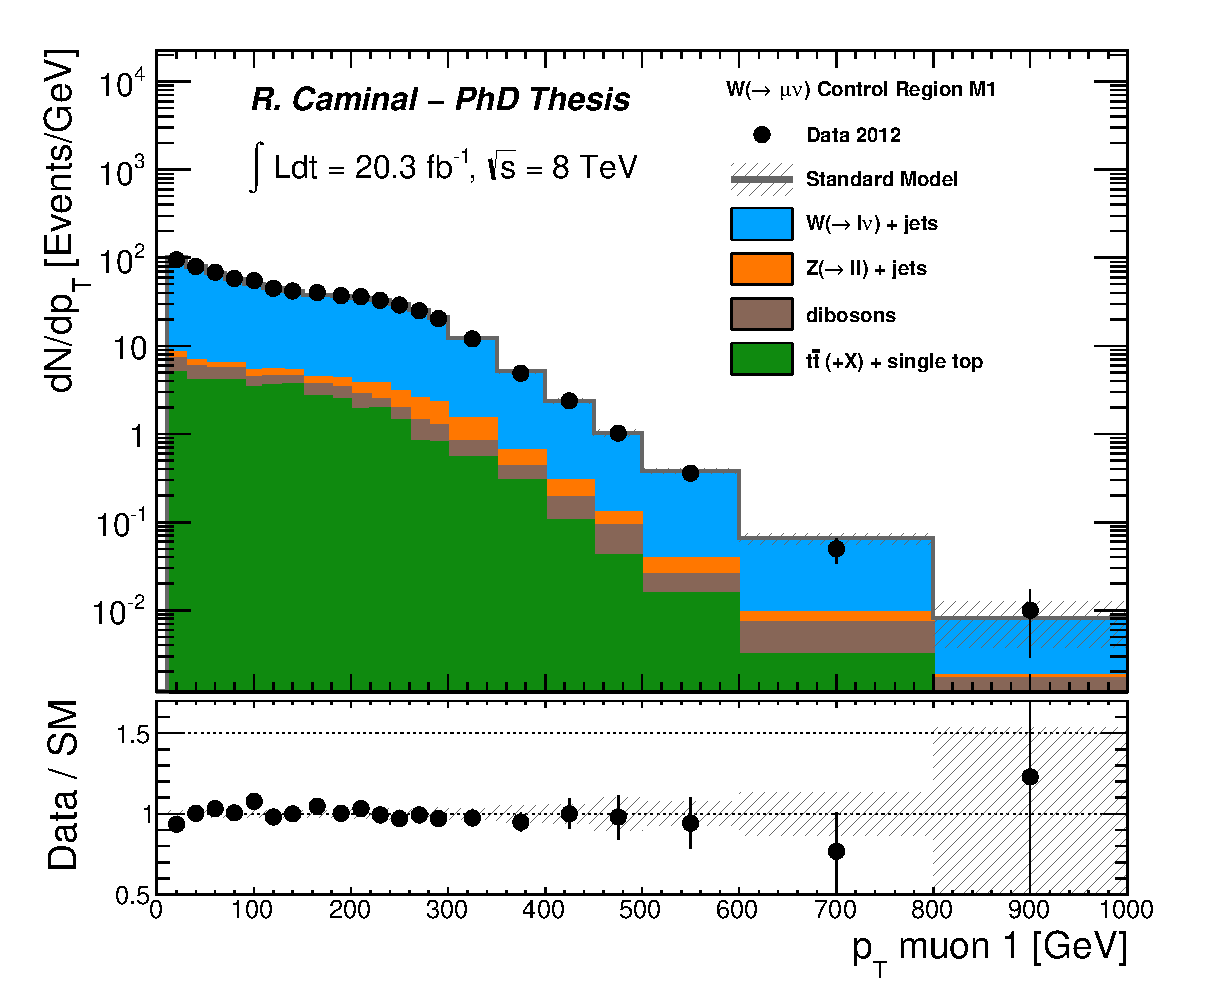
\includegraphics[width=0.495\textwidth]{MonojetAnalysis/Figures/plot_Stop_A6_CRwmn_m_pt_fitted.eps}
      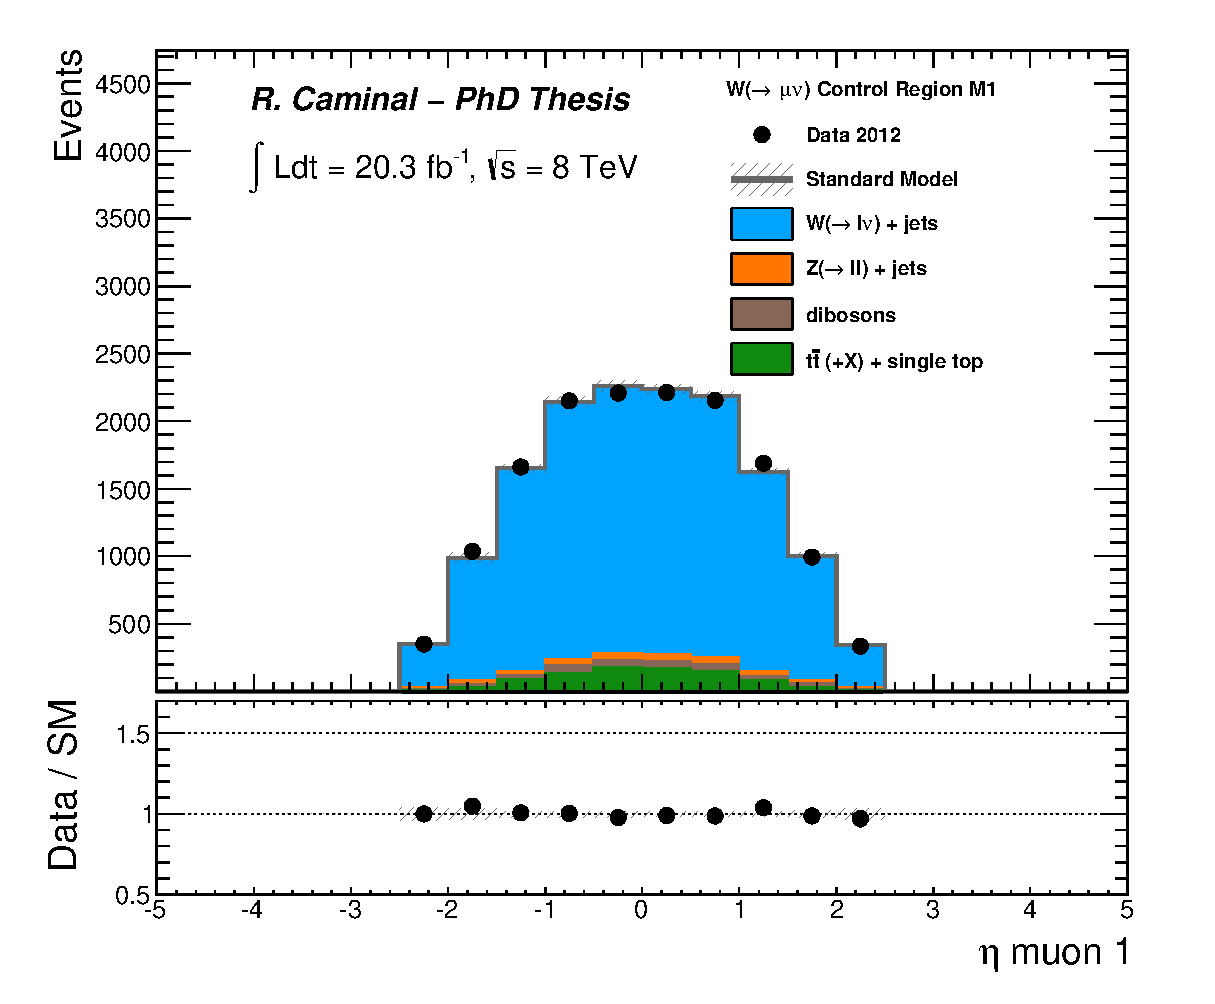
\includegraphics[width=0.495\textwidth]{MonojetAnalysis/Figures/plot_Stop_A6_CRwmn_m_eta_fitted.eps}
    }
    \mbox{
      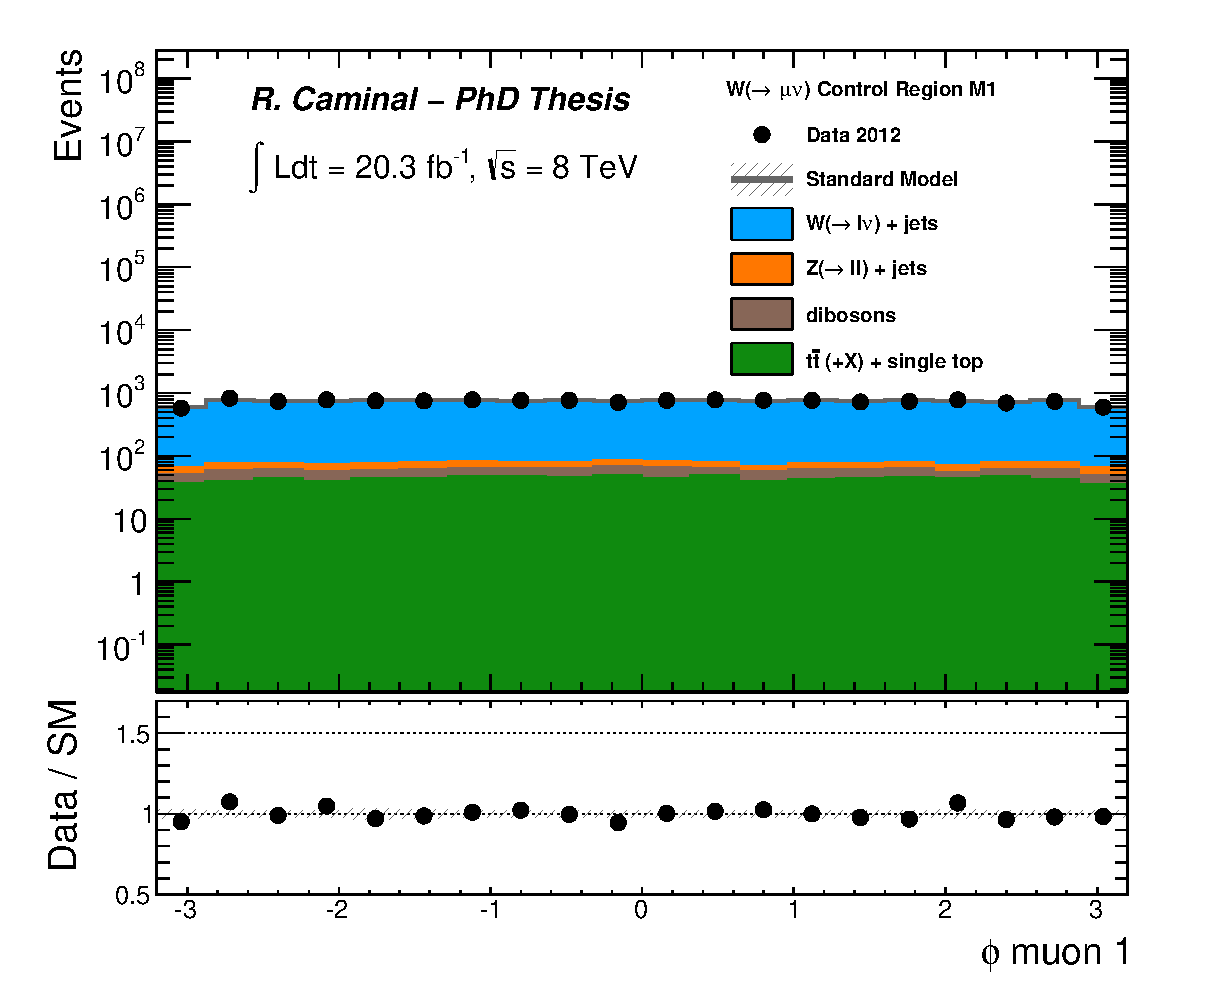
\includegraphics[width=0.495\textwidth]{MonojetAnalysis/Figures/plot_Stop_A6_CRwmn_m_phi_fitted.eps}
      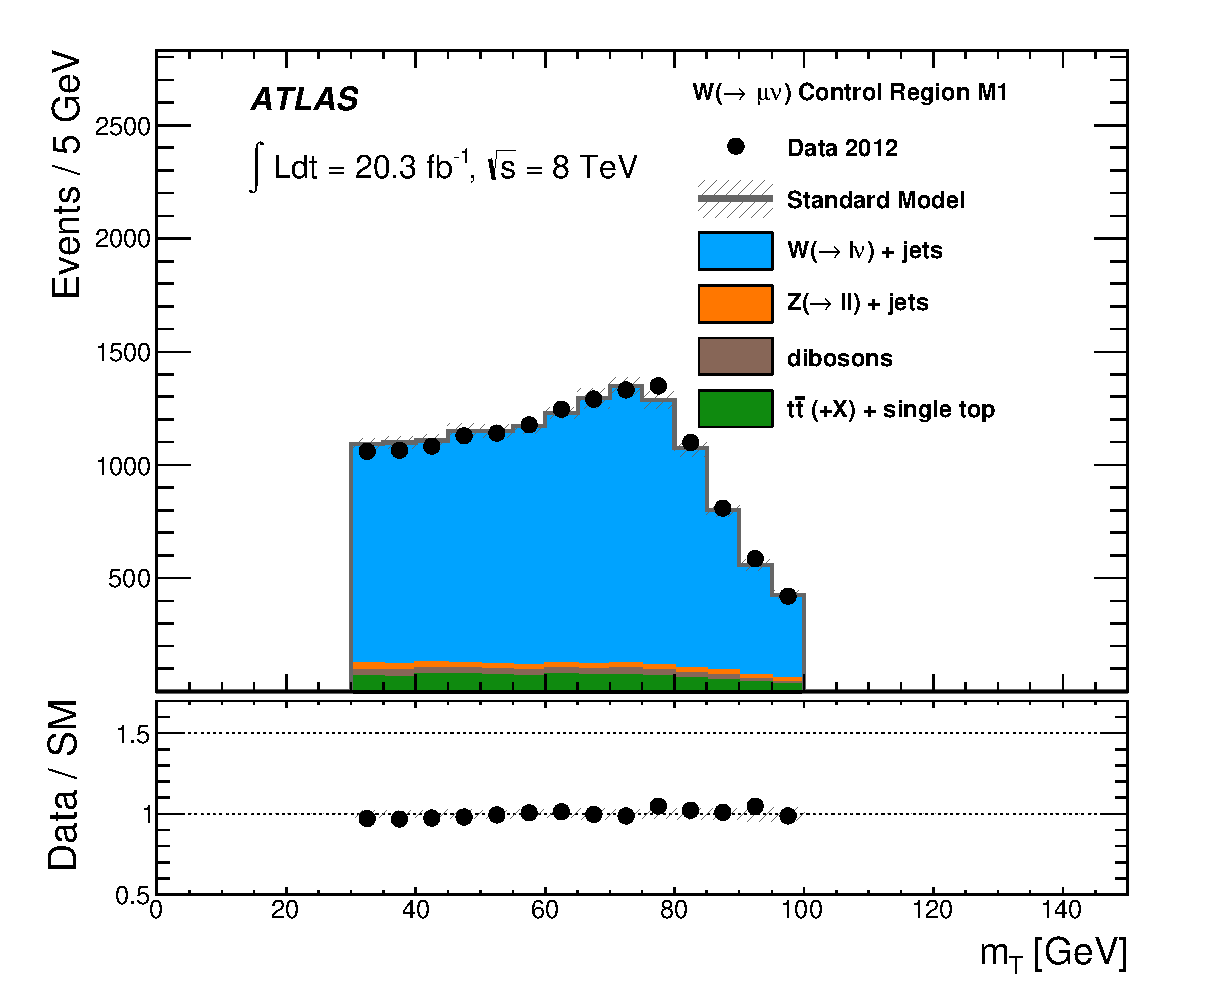
\includegraphics[width=0.495\textwidth]{MonojetAnalysis/Figures/plot_Stop_A6_CRwmn_m_MT_fitted.eps}
    }
  \end{center}
  \caption[Kinematic distributions of the identified muons in the $\wmn$+jets control region for the selection cuts of region M1, after the normalization factors extracted from the fit have been applied.]{The measured kinematic distributions of the identified muons in the $\wmn$+jets control region for the selection cuts of region M1 compared to the background predictions. The latter include the global normalization factors extracted from the fit. The error bands in the ratios include the statistical and experimental uncertainties on the background predictions.}
  \label{fig:Plot_M1_CRwmn_Leptonkinematics}
\end{figure}

\begin{figure}[!ht]
  \begin{center}
    \mbox{
      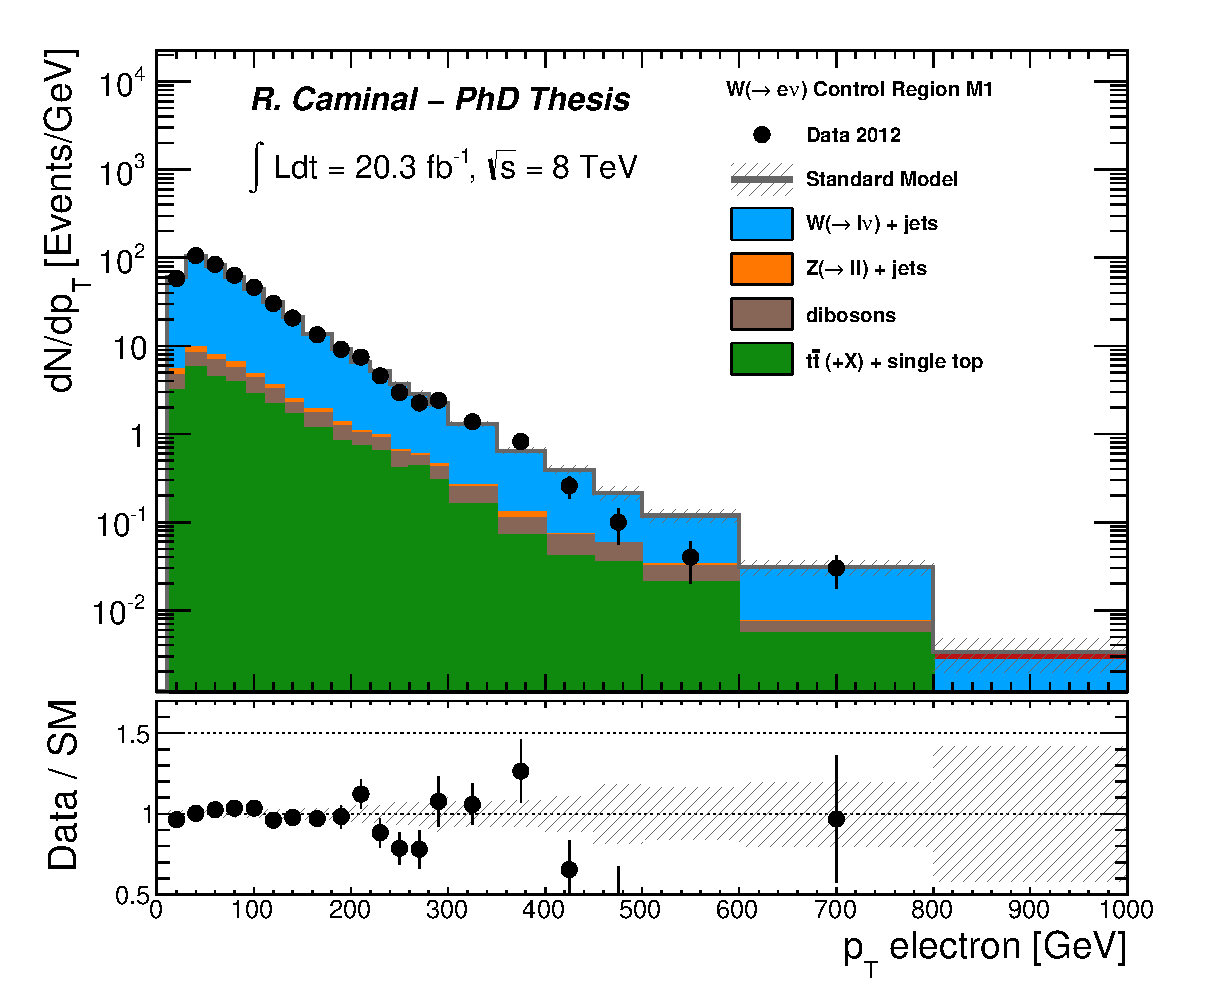
\includegraphics[width=0.495\textwidth]{MonojetAnalysis/Figures/plot_Stop_A6_CRele_e_pt_fitted.eps}
      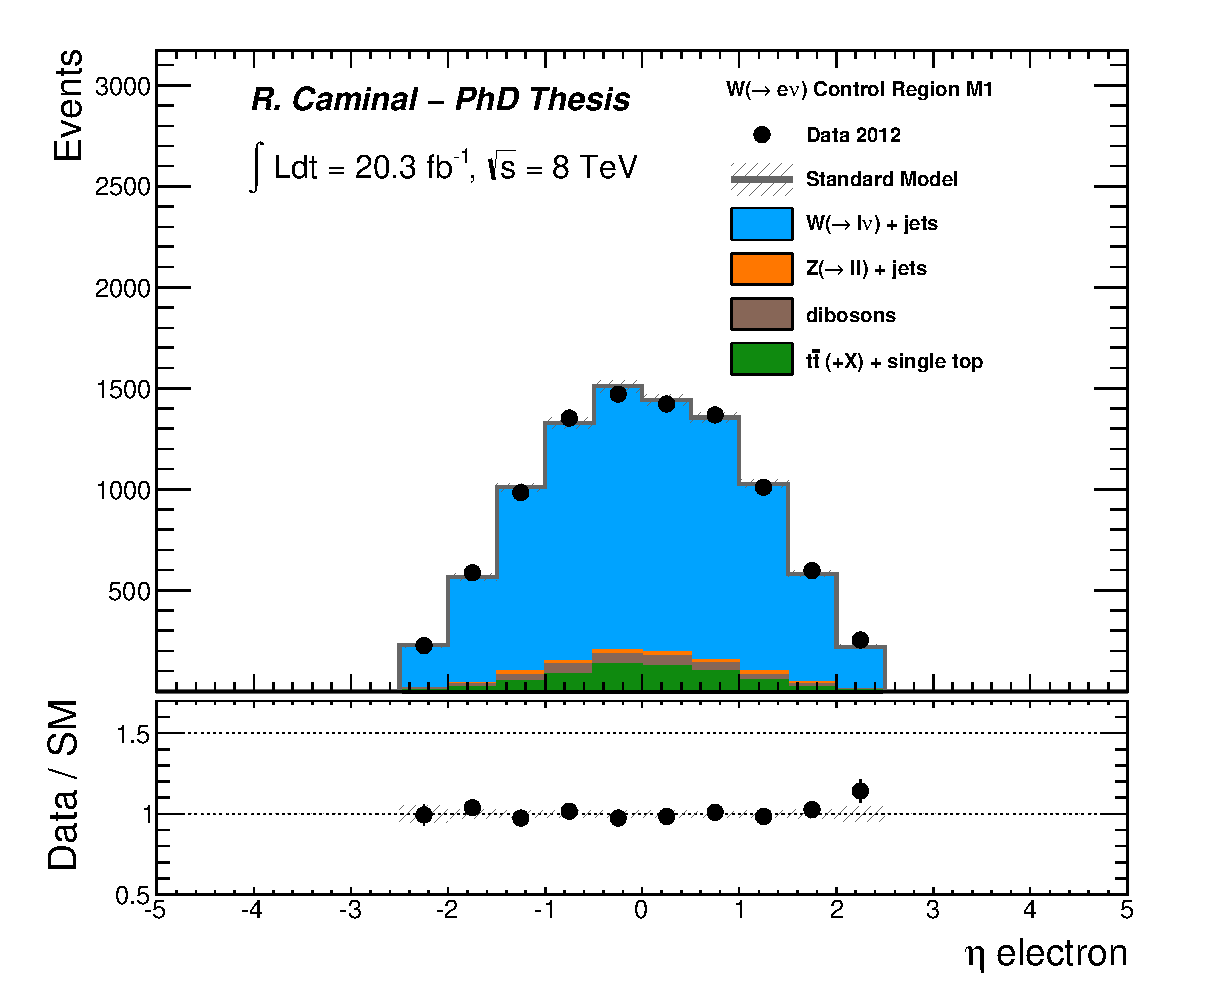
\includegraphics[width=0.495\textwidth]{MonojetAnalysis/Figures/plot_Stop_A6_CRele_e_eta_fitted.eps}
    }
    \mbox{
      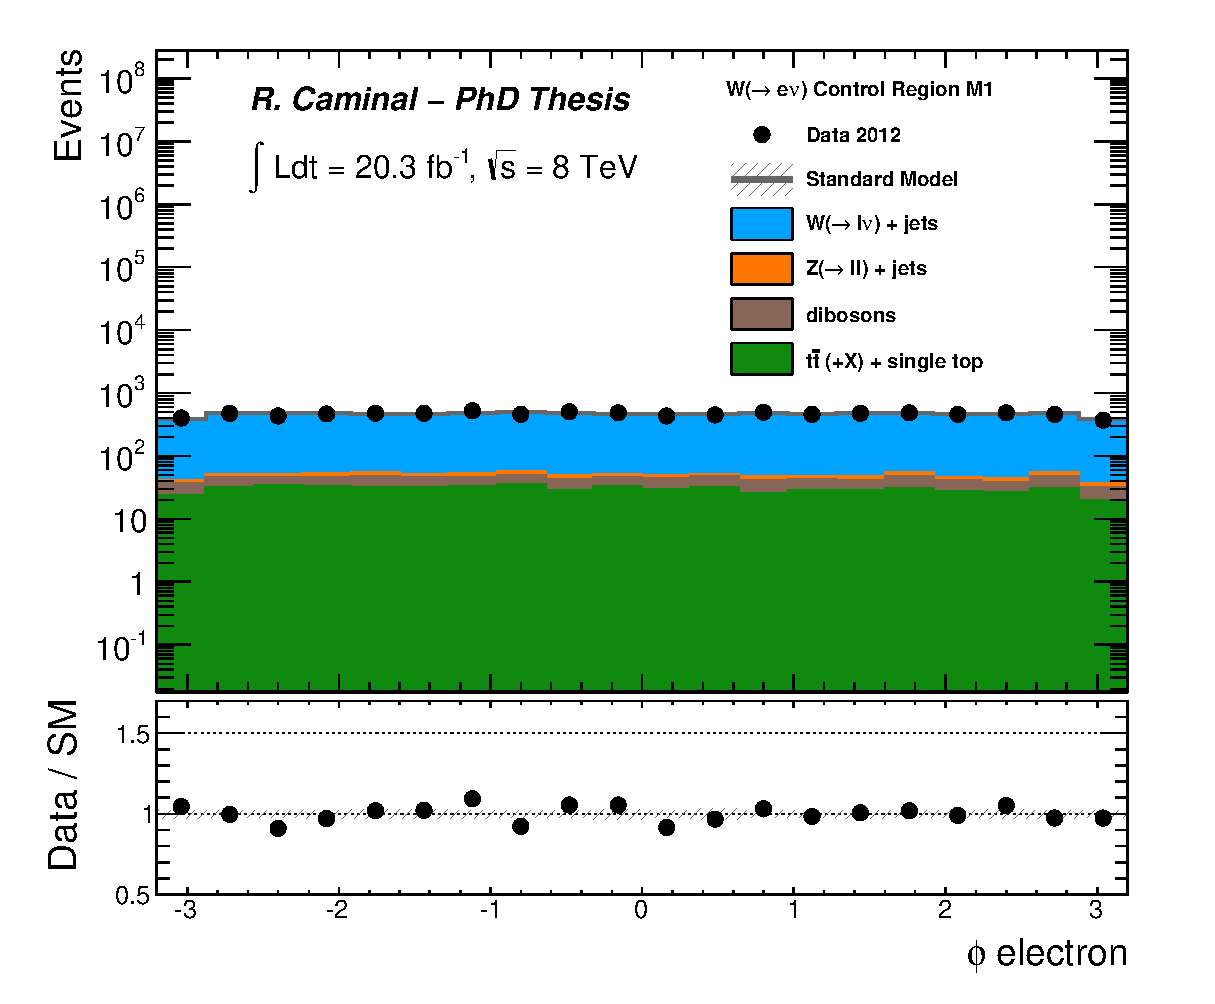
\includegraphics[width=0.495\textwidth]{MonojetAnalysis/Figures/plot_Stop_A6_CRele_e_phi_fitted.eps}
      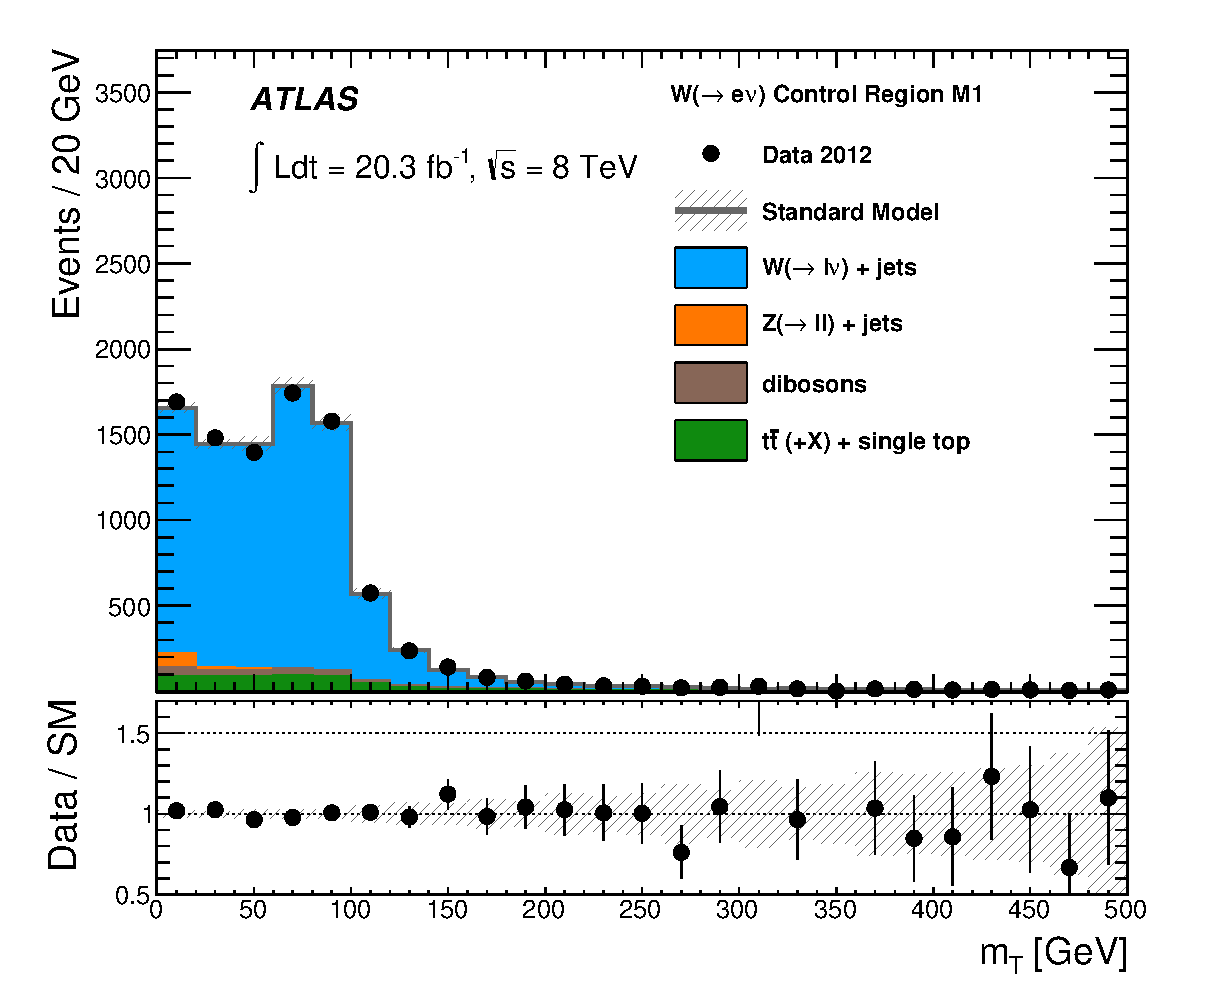
\includegraphics[width=0.495\textwidth]{MonojetAnalysis/Figures/plot_Stop_A6_CRele_e_MT_fitted.eps}
    }
  \end{center}
  \caption[Kinematic distributions of the identified electrons in the $\wen$+jets control region for the selection cuts of region M1, after the normalization factors extracted from the fit have been applied.]{The measured kinematic distributions of the identified electrons in the $\wen$+jets control region for the selection cuts of region M1 compared to the background predictions. The latter include the global normalization factors extracted from the fit. The error bands in the ratios include the statistical and experimental uncertainties on the background predictions.}
  \label{fig:Plot_M1_CRele_Leptonkinematics}
\end{figure}

\begin{figure}[!ht]
  \begin{center}
    \mbox{
      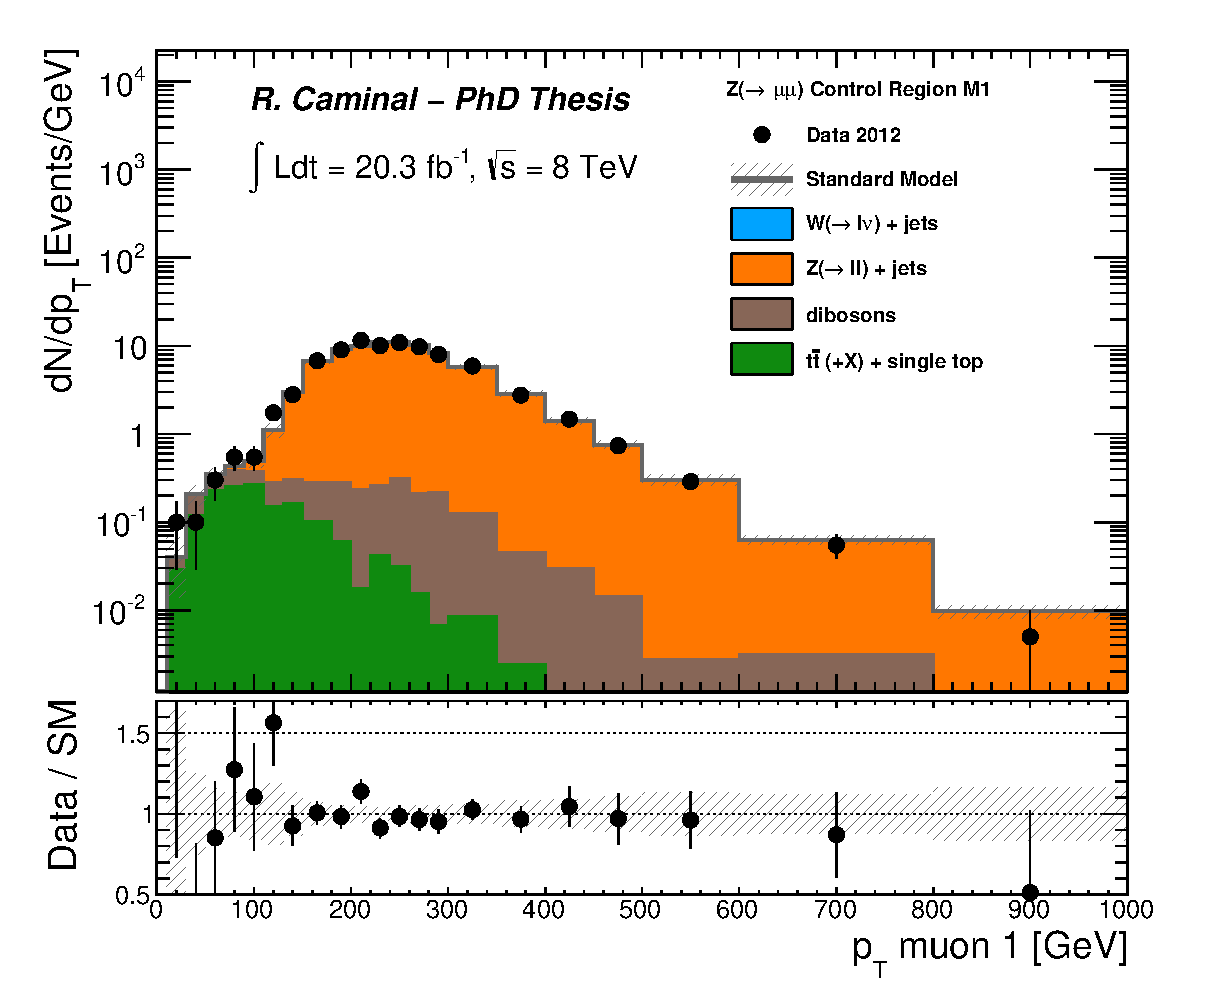
\includegraphics[width=0.495\textwidth]{MonojetAnalysis/Figures/plot_Stop_A6_CRzmm_m_pt_fitted.eps}
      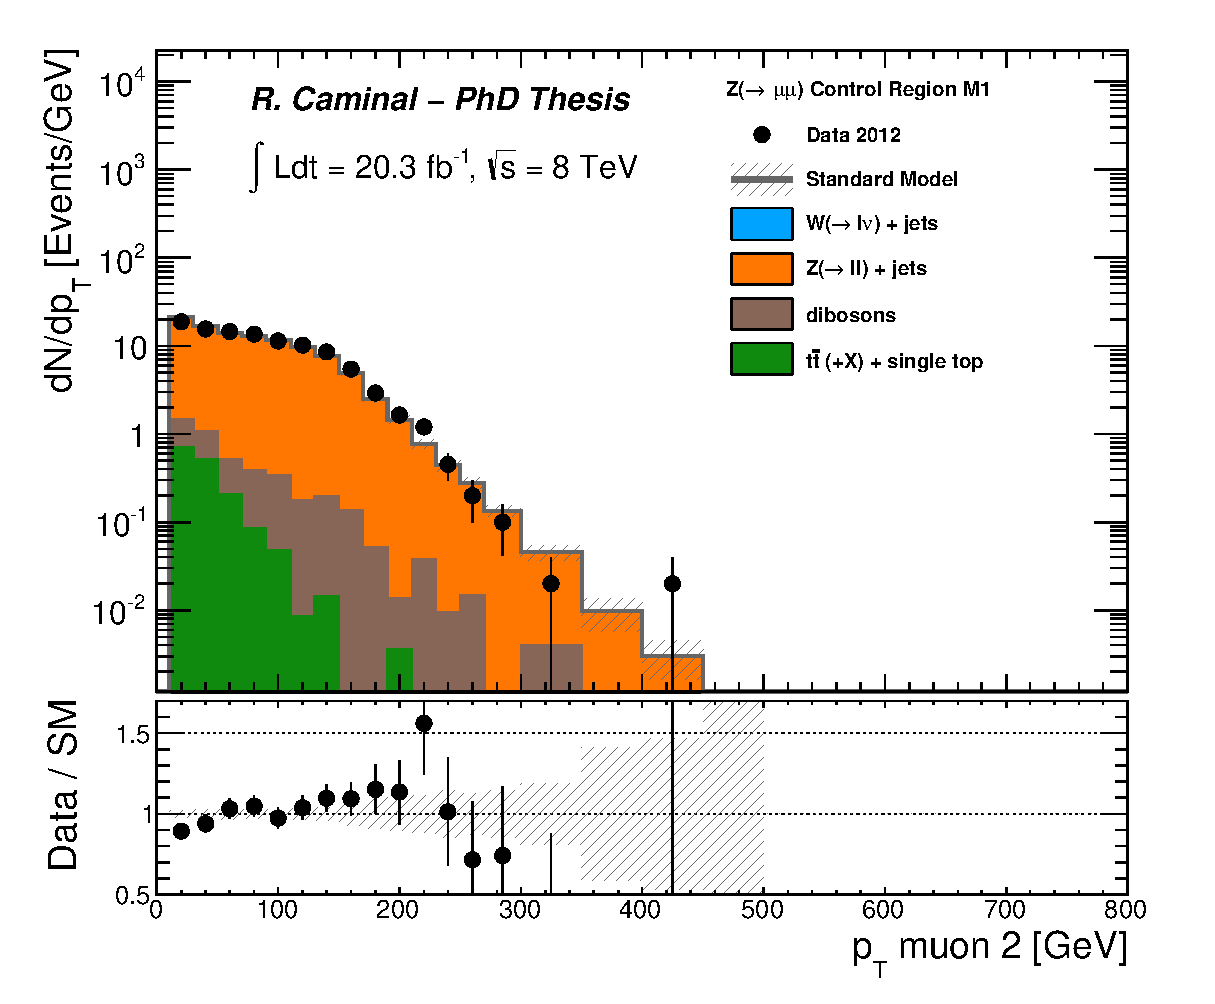
\includegraphics[width=0.495\textwidth]{MonojetAnalysis/Figures/plot_Stop_A6_CRzmm_m2_pt_fitted.eps}
    }
    \mbox{
      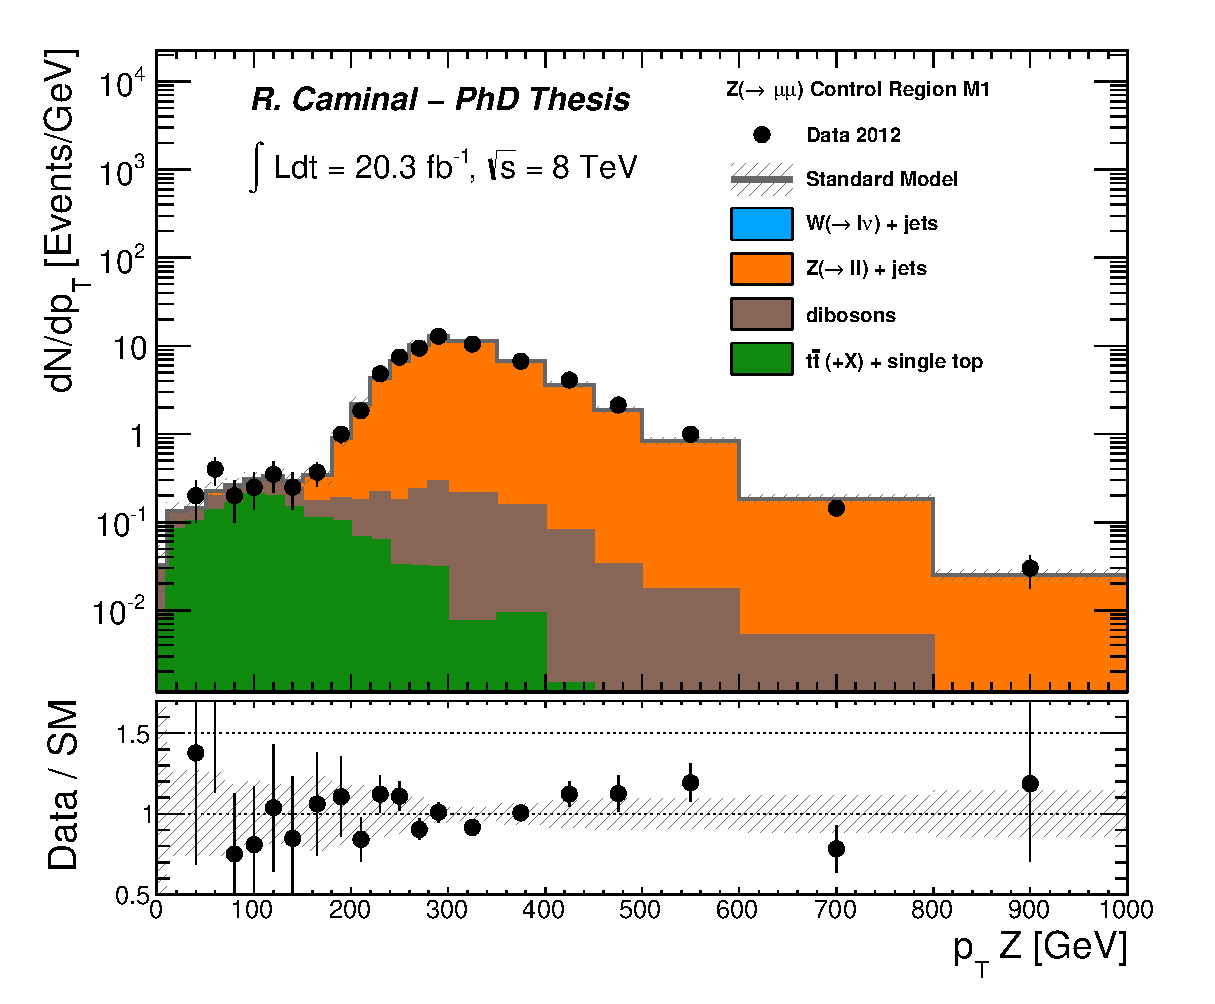
\includegraphics[width=0.495\textwidth]{MonojetAnalysis/Figures/plot_Stop_A6_CRzmm_m_Zpt_fitted.eps}
      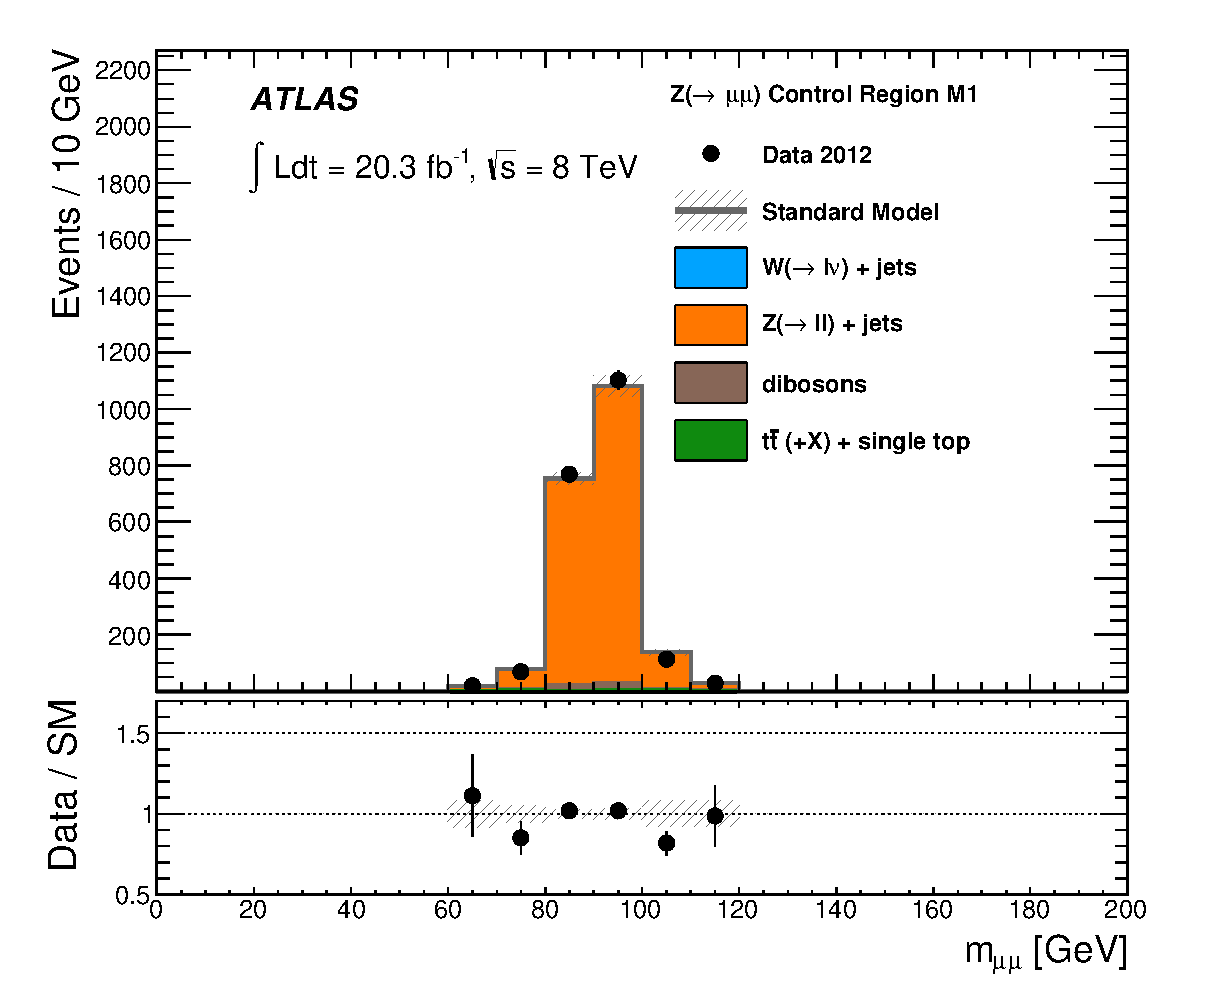
\includegraphics[width=0.495\textwidth]{MonojetAnalysis/Figures/plot_Stop_A6_CRzmm_m_M_fitted.eps}
    }
  \end{center}
  \caption[Kinematic distributions of the identified muons in the $Z/\gamma^{\ast}(\rightarrow \mu^{+}\mu^{-})$+jets control region for the selection cuts of region M1, after the normalization factors extracted from the fit have been applied.]{The measured kinematic distributions of the identified muons in the $\zmm$+jets control region for the selection cuts of region M1 compared to the background predictions. The latter include the global normalization factors extracted from the fit. The error bands in the ratios include the statistical and experimental uncertainties on the background predictions.}
  \label{fig:Plot_M1_CRzmm_Leptonkinematics}
\end{figure}

\begin{figure}[!ht]
  \begin{center}
    \mbox{
      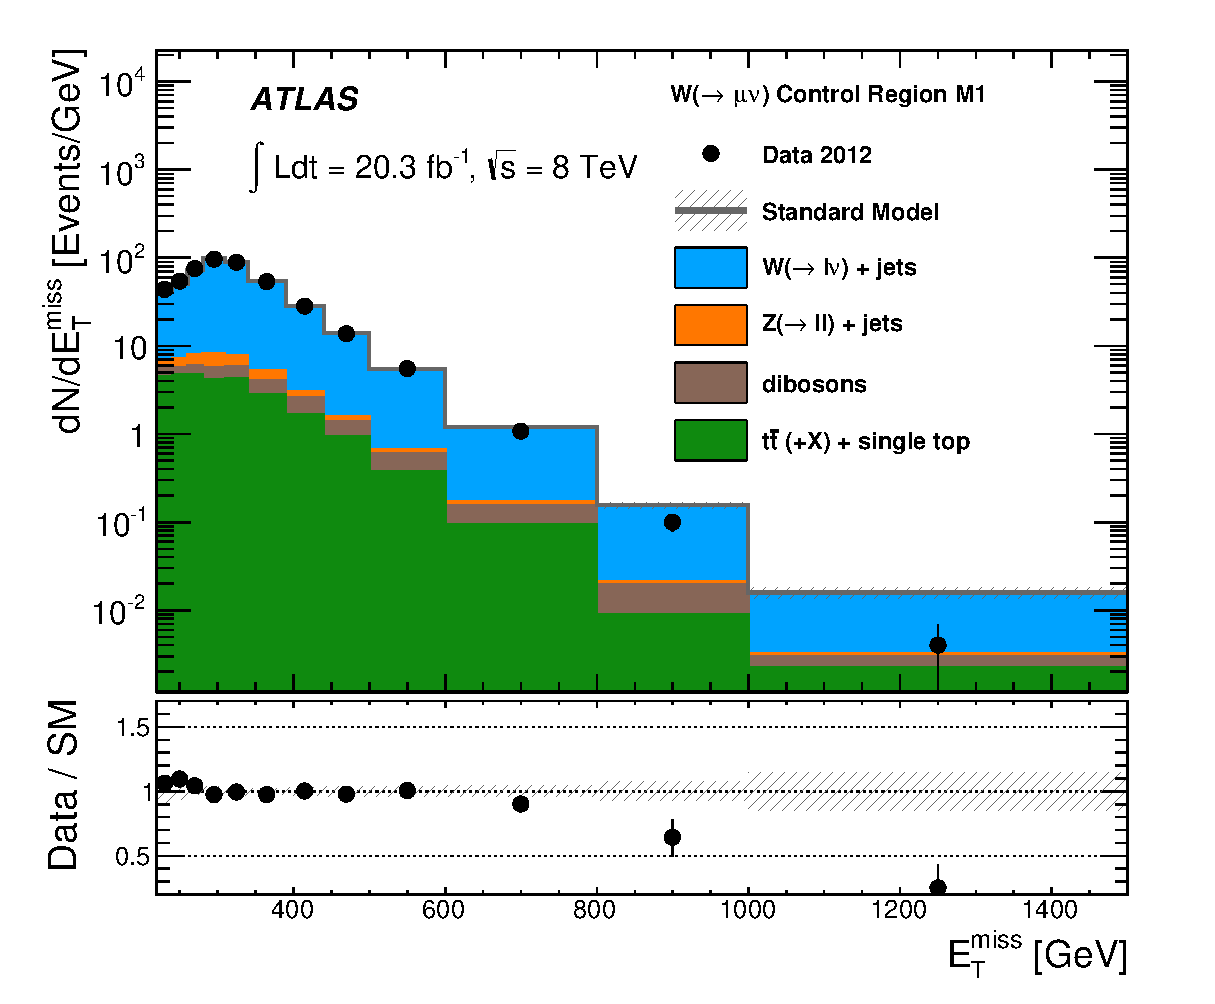
\includegraphics[width=0.495\textwidth]{MonojetAnalysis/Figures/plot_Stop_A6_CRwmn_met_fitted.eps}
      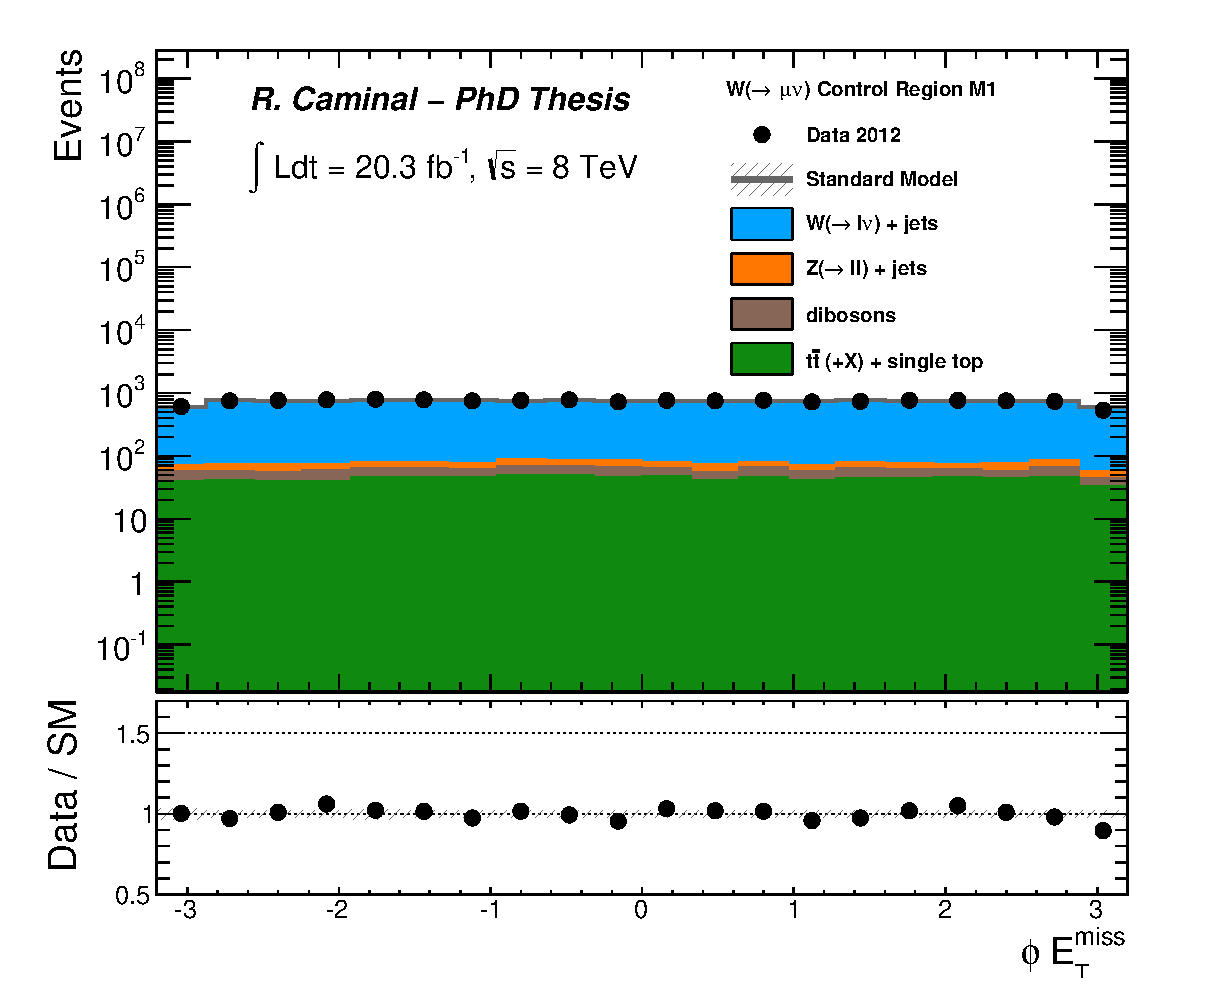
\includegraphics[width=0.495\textwidth]{MonojetAnalysis/Figures/plot_Stop_A6_CRwmn_met_phi_fitted.eps}
    }
    \mbox{
      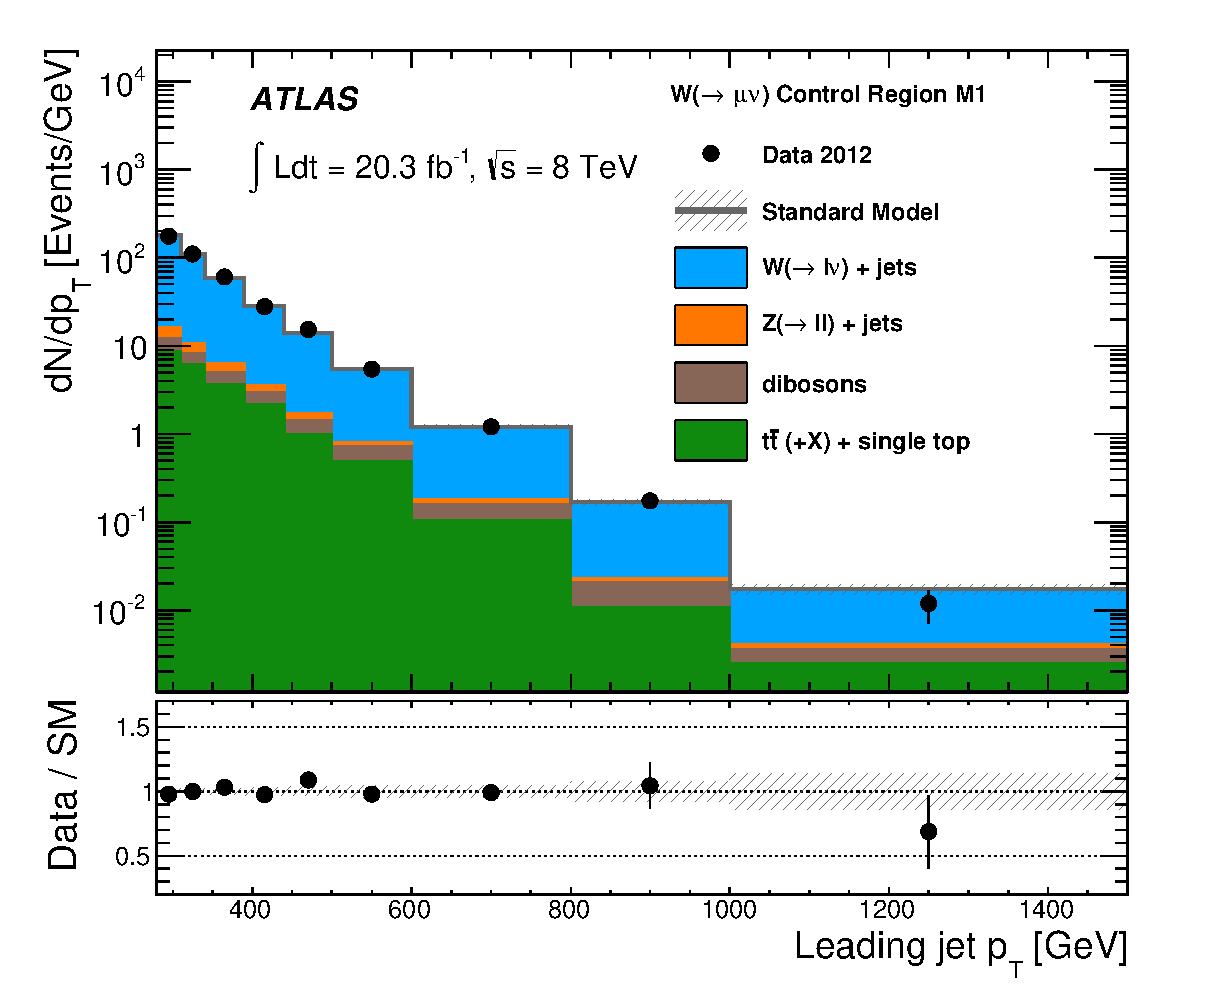
\includegraphics[width=0.495\textwidth]{MonojetAnalysis/Figures/plot_Stop_A6_CRwmn_pt1_fitted.eps}
      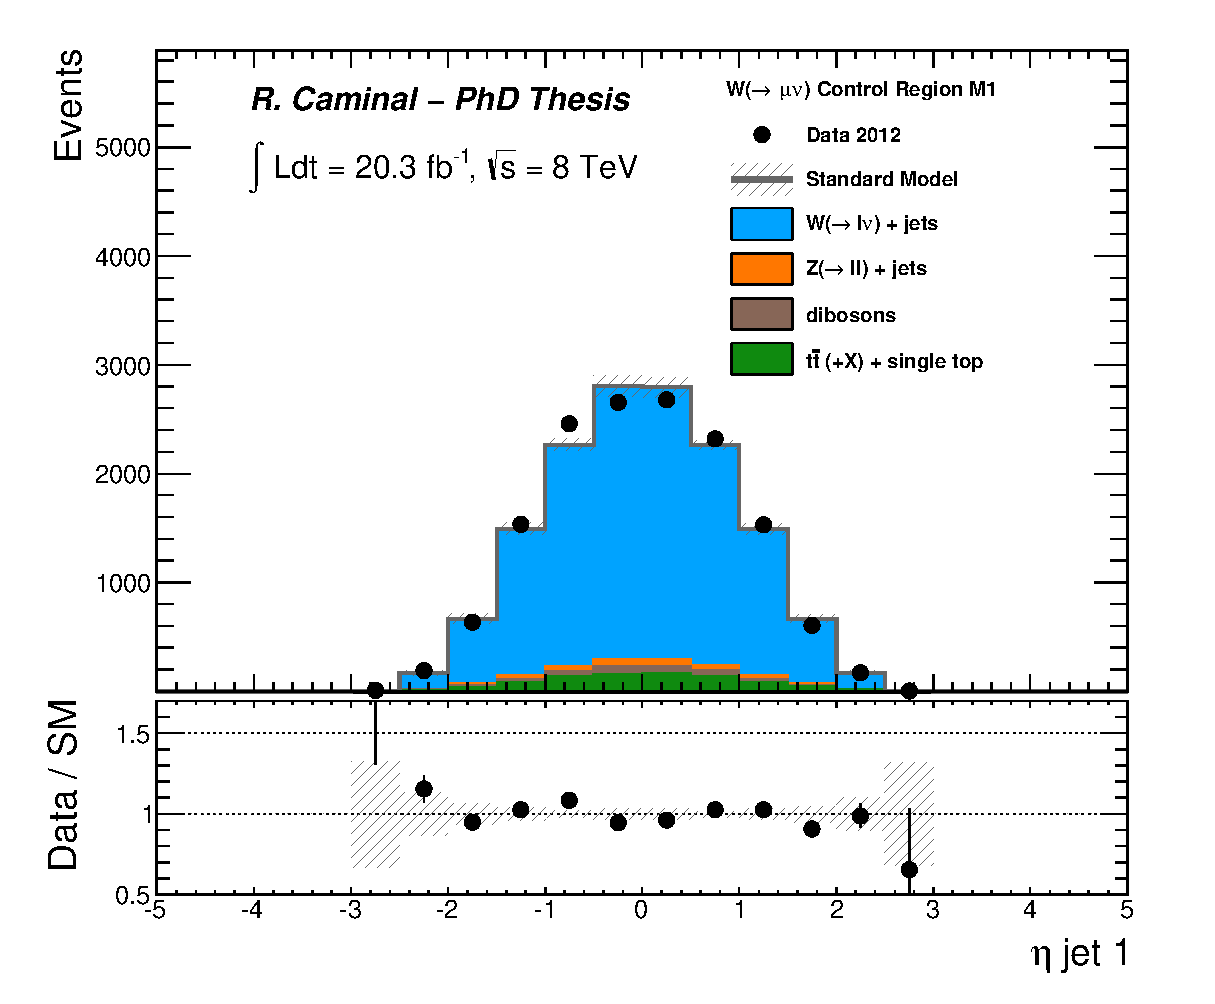
\includegraphics[width=0.495\textwidth]{MonojetAnalysis/Figures/plot_Stop_A6_CRwmn_eta1_fitted.eps}
    }
    \mbox{
      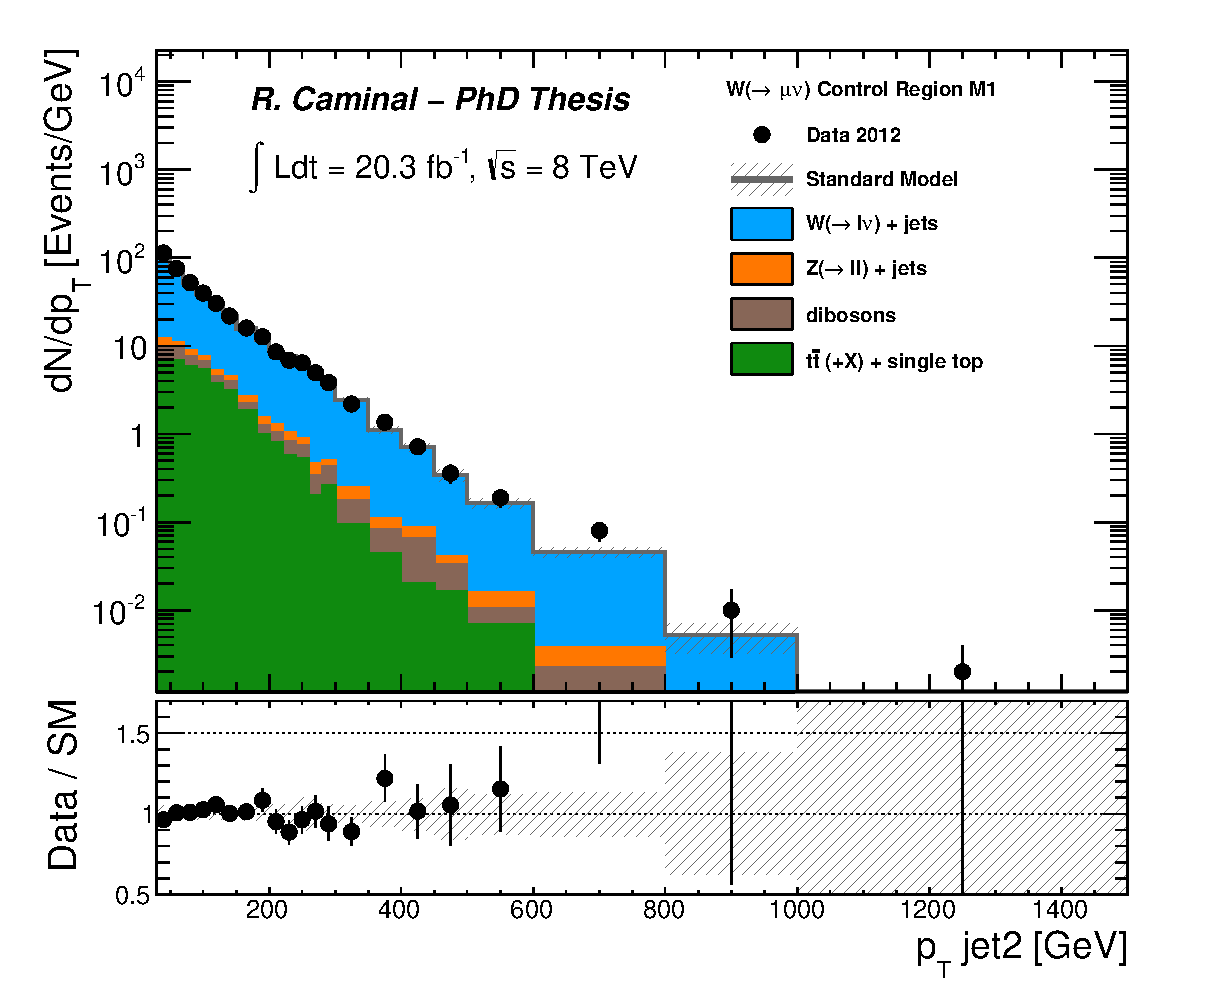
\includegraphics[width=0.495\textwidth]{MonojetAnalysis/Figures/plot_Stop_A6_CRwmn_pt2_fitted.eps}
      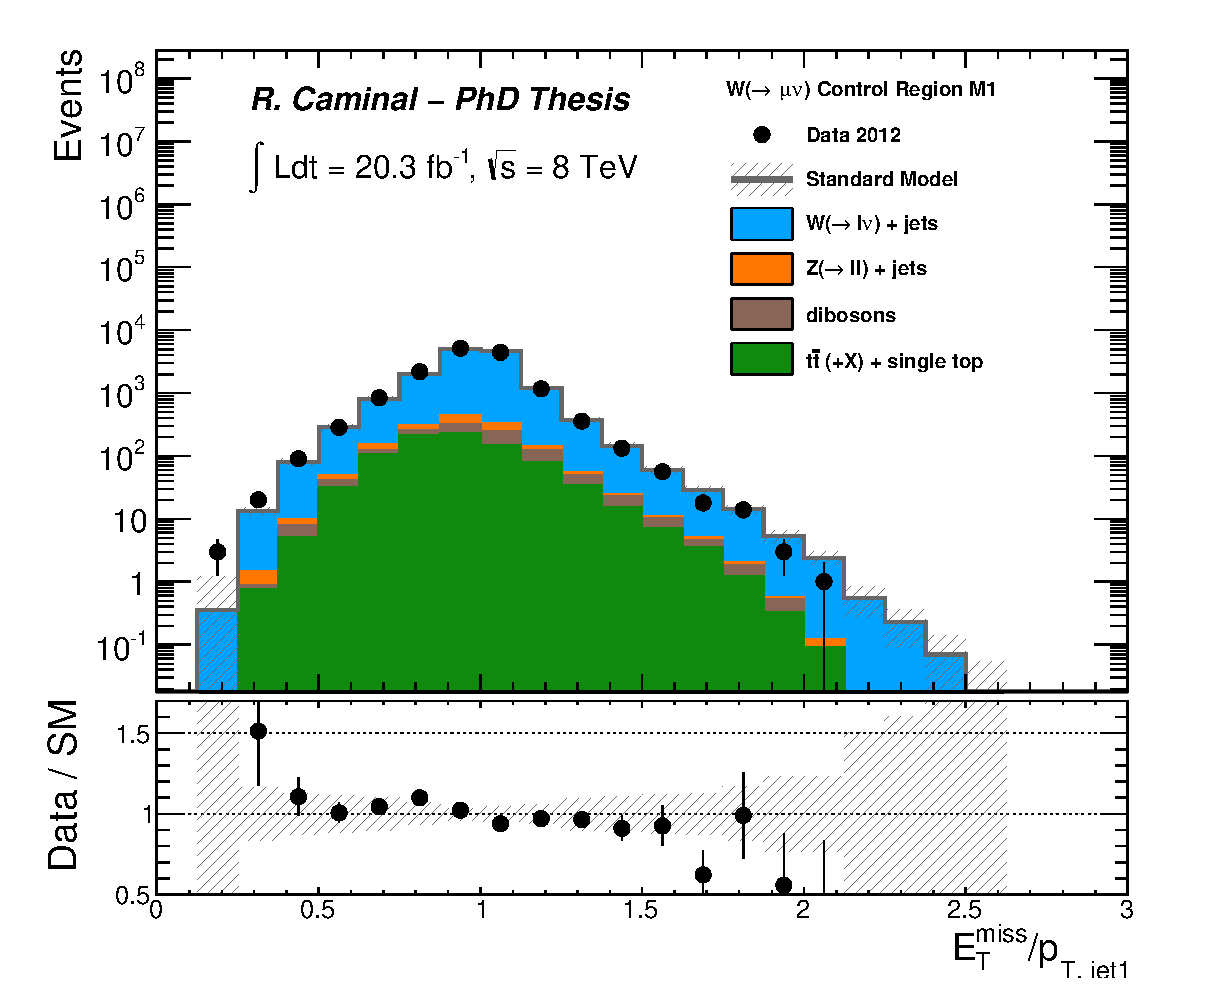
\includegraphics[width=0.495\textwidth]{MonojetAnalysis/Figures/plot_Stop_A6_CRwmn_metpt1_fitted.eps}
    }
  \end{center}
  \caption[Kinematic distributions of the reconstructed jets and $\met$ in the $\wmn$ control region for the selection cuts of region M1, after the normalization factors extracted from the fit have been applied.]{The measured kinematic distributions of the reconstructed jets and $\met$ in the $\wmn$ control region for the selection cuts of region M1 compared to the background predictions. The latter include the global normalization factors extracted from the fit. The error bands in the ratios include the statistical and experimental uncertainties on the background predictions.}
  \label{fig:Plot_M1_CRwmn_Jetkinematics}
\end{figure}

\begin{figure}[!ht]
  \begin{center}
    \mbox{
      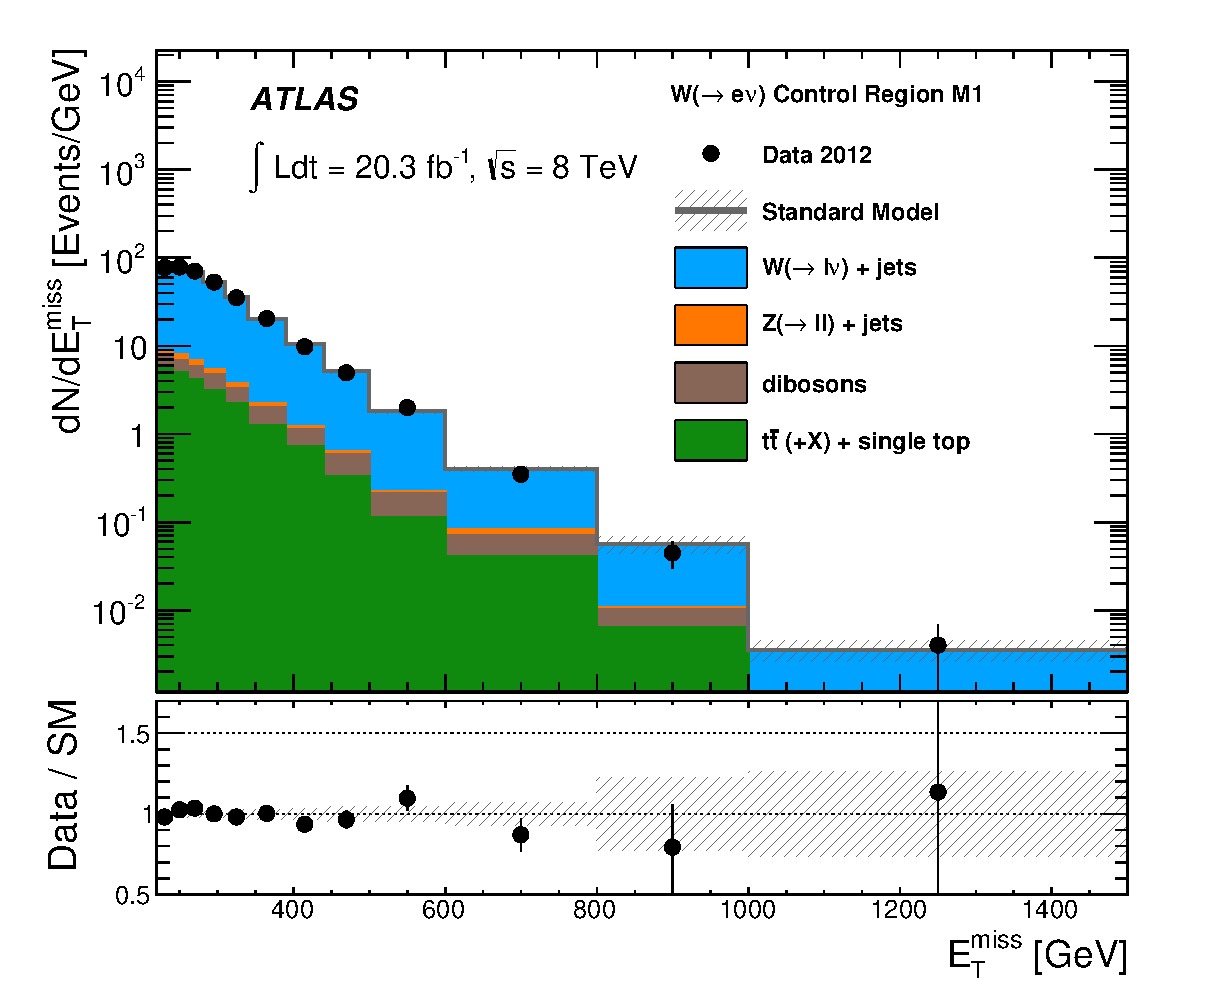
\includegraphics[width=0.495\textwidth]{MonojetAnalysis/Figures/plot_Stop_A6_CRele_met_fitted.eps}
      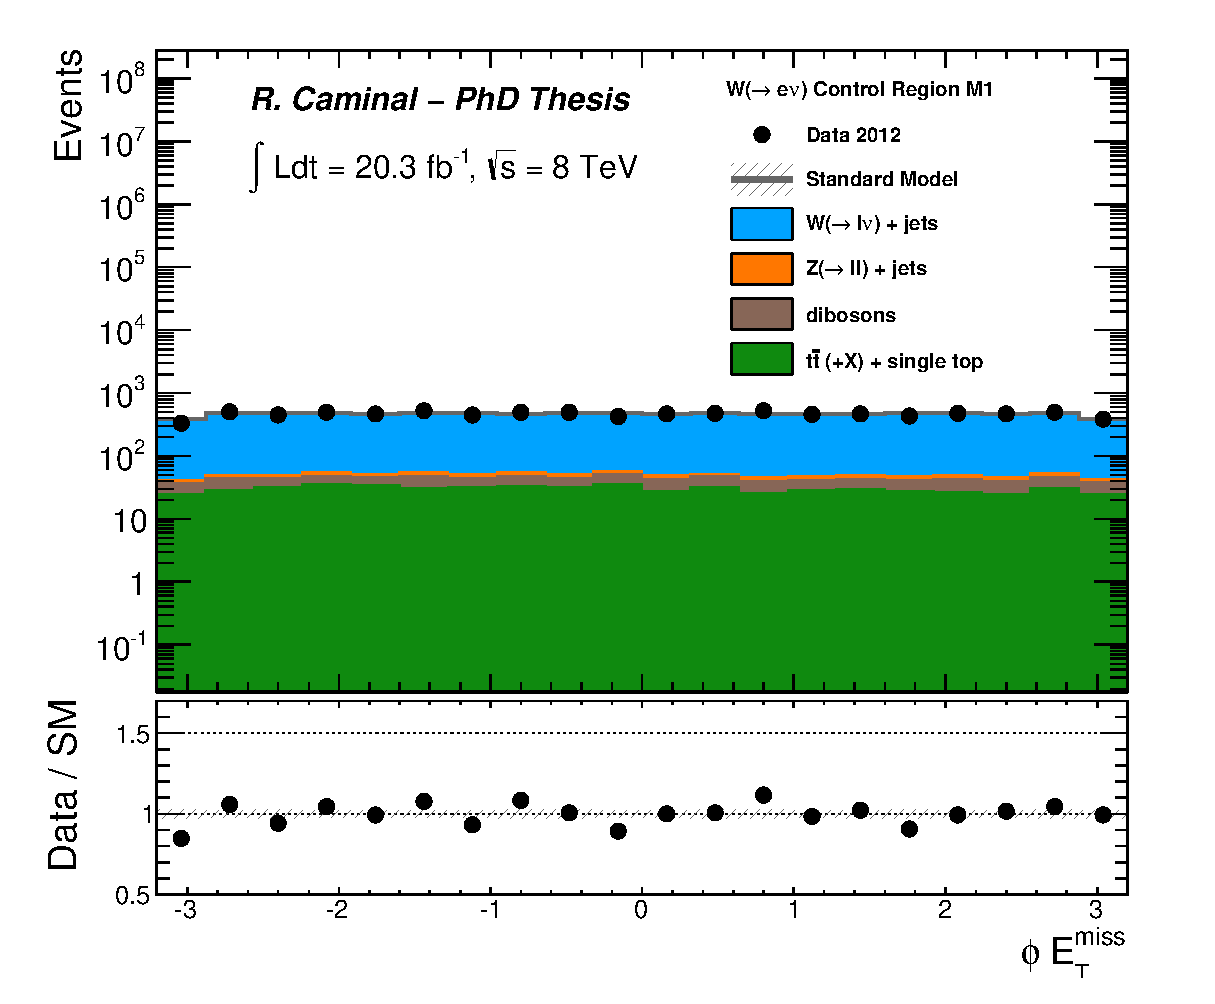
\includegraphics[width=0.495\textwidth]{MonojetAnalysis/Figures/plot_Stop_A6_CRele_met_phi_fitted.eps}
    }
    \mbox{
      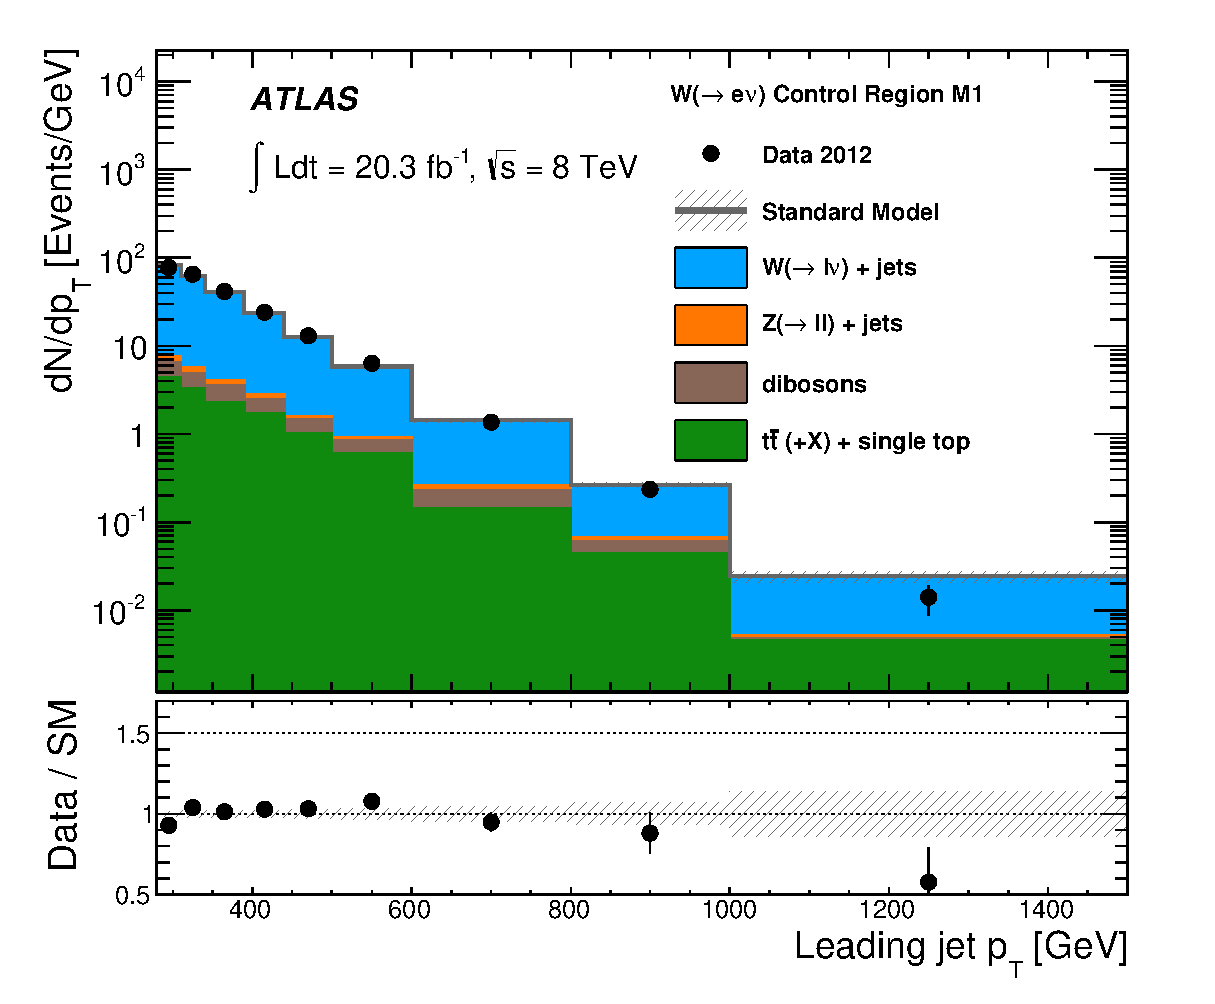
\includegraphics[width=0.495\textwidth]{MonojetAnalysis/Figures/plot_Stop_A6_CRele_pt1_fitted.eps}
      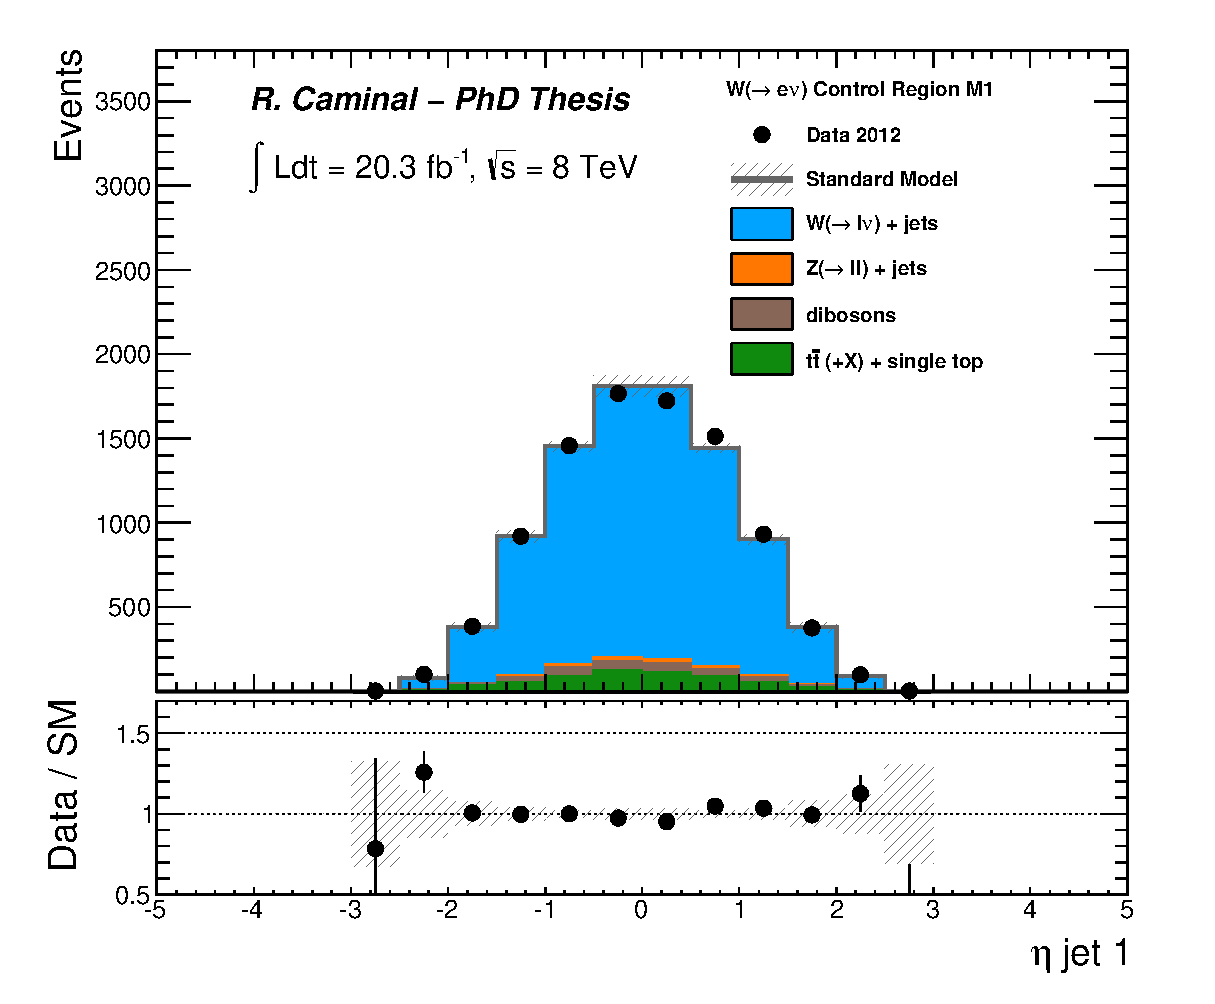
\includegraphics[width=0.495\textwidth]{MonojetAnalysis/Figures/plot_Stop_A6_CRele_eta1_fitted.eps}
    }
    \mbox{
      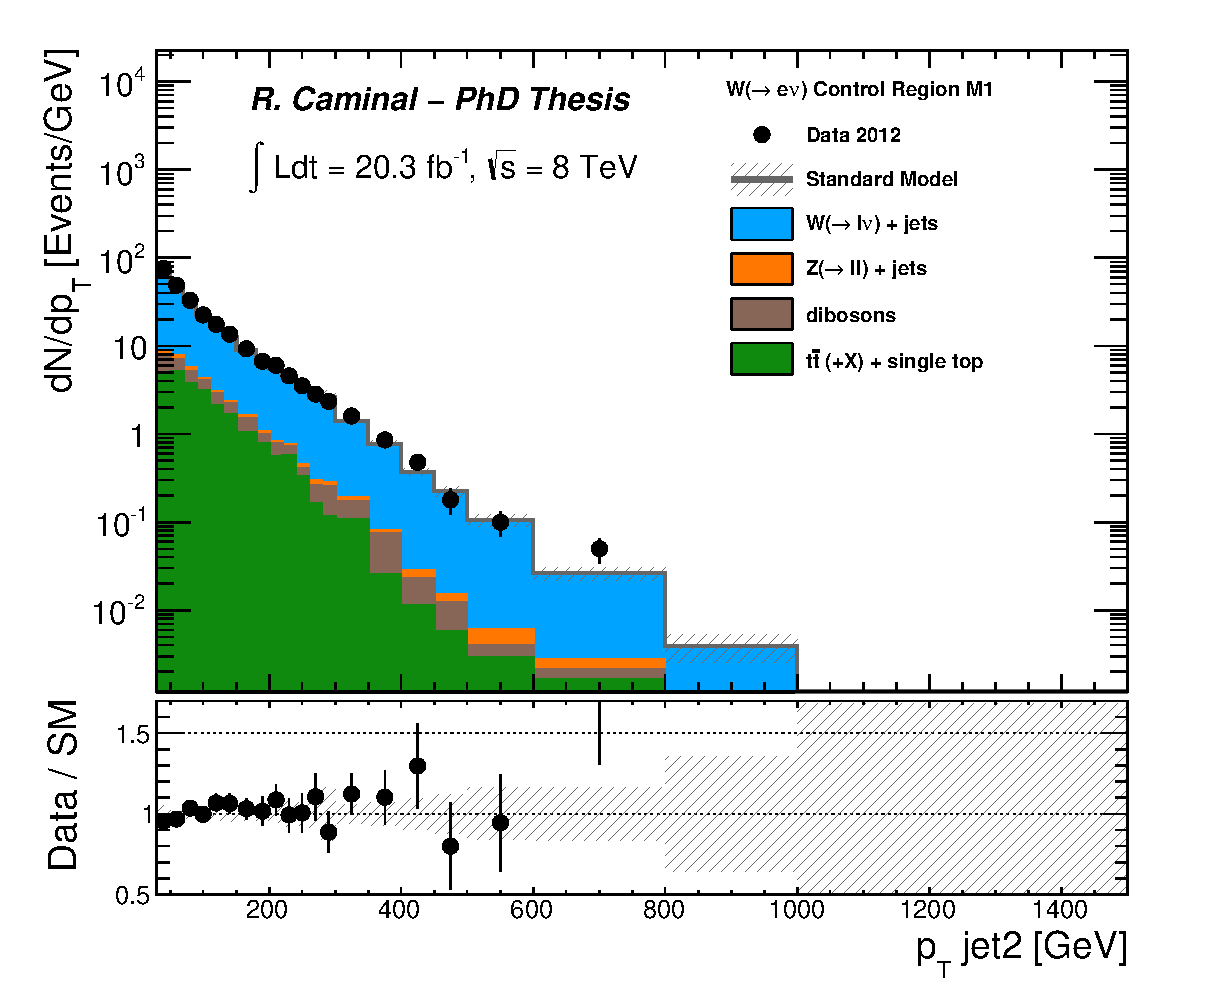
\includegraphics[width=0.495\textwidth]{MonojetAnalysis/Figures/plot_Stop_A6_CRele_pt2_fitted.eps}
      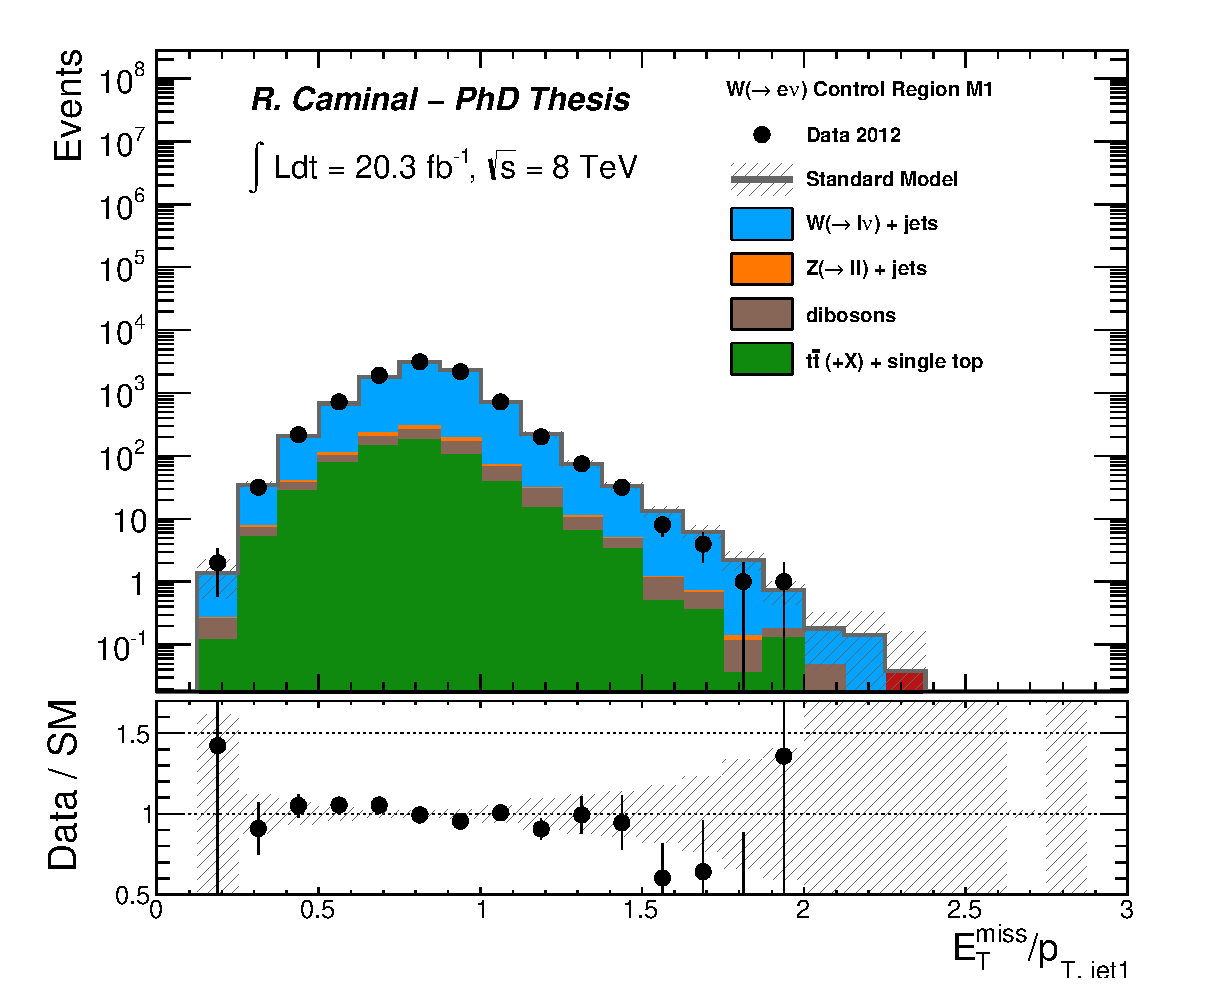
\includegraphics[width=0.495\textwidth]{MonojetAnalysis/Figures/plot_Stop_A6_CRele_metpt1_fitted.eps}
    }
  \end{center}
  \caption[Kinematic distributions of the reconstructed jets and $\met$ in the $\wen$+jets control region for the selection cuts of region M1, after the normalization factors extracted from the fit have been applied.]{The measured kinematic distributions of the reconstructed jets and $\met$ in the $\wen$+jets control region for the selection cuts of region M1 compared to the background predictions. The latter include the global normalization factors extracted from the fit. The error bands in the ratios include the statistical and experimental uncertainties on the background predictions.}
  \label{fig:Plot_M1_CRele_Jetkinematics}
\end{figure}

\begin{figure}[!ht]
  \begin{center}
    \mbox{
      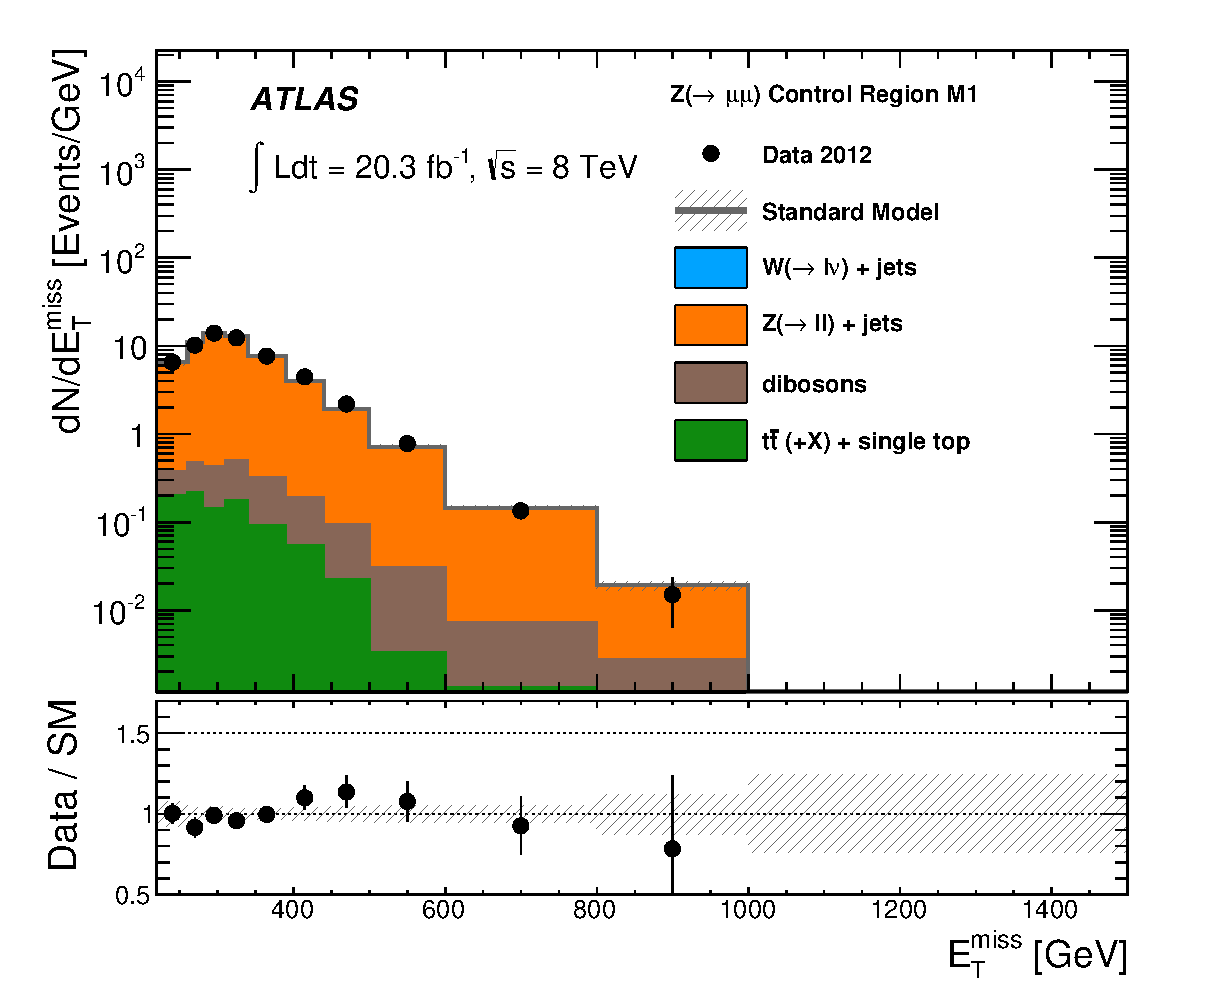
\includegraphics[width=0.495\textwidth]{MonojetAnalysis/Figures/plot_Stop_A6_CRzmm_met_fitted.eps}
      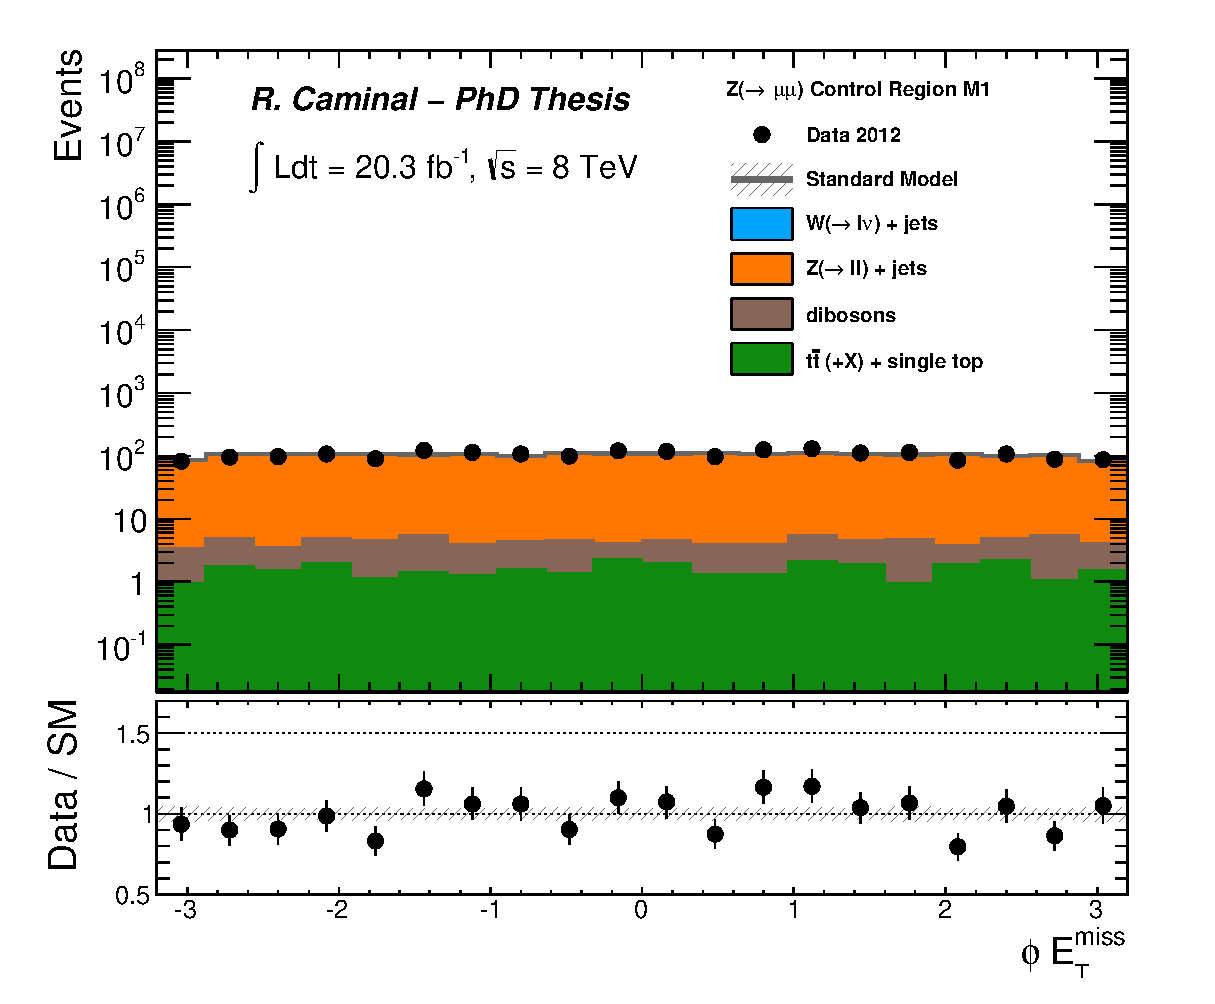
\includegraphics[width=0.495\textwidth]{MonojetAnalysis/Figures/plot_Stop_A6_CRzmm_met_phi_fitted.eps}
    }
    \mbox{
      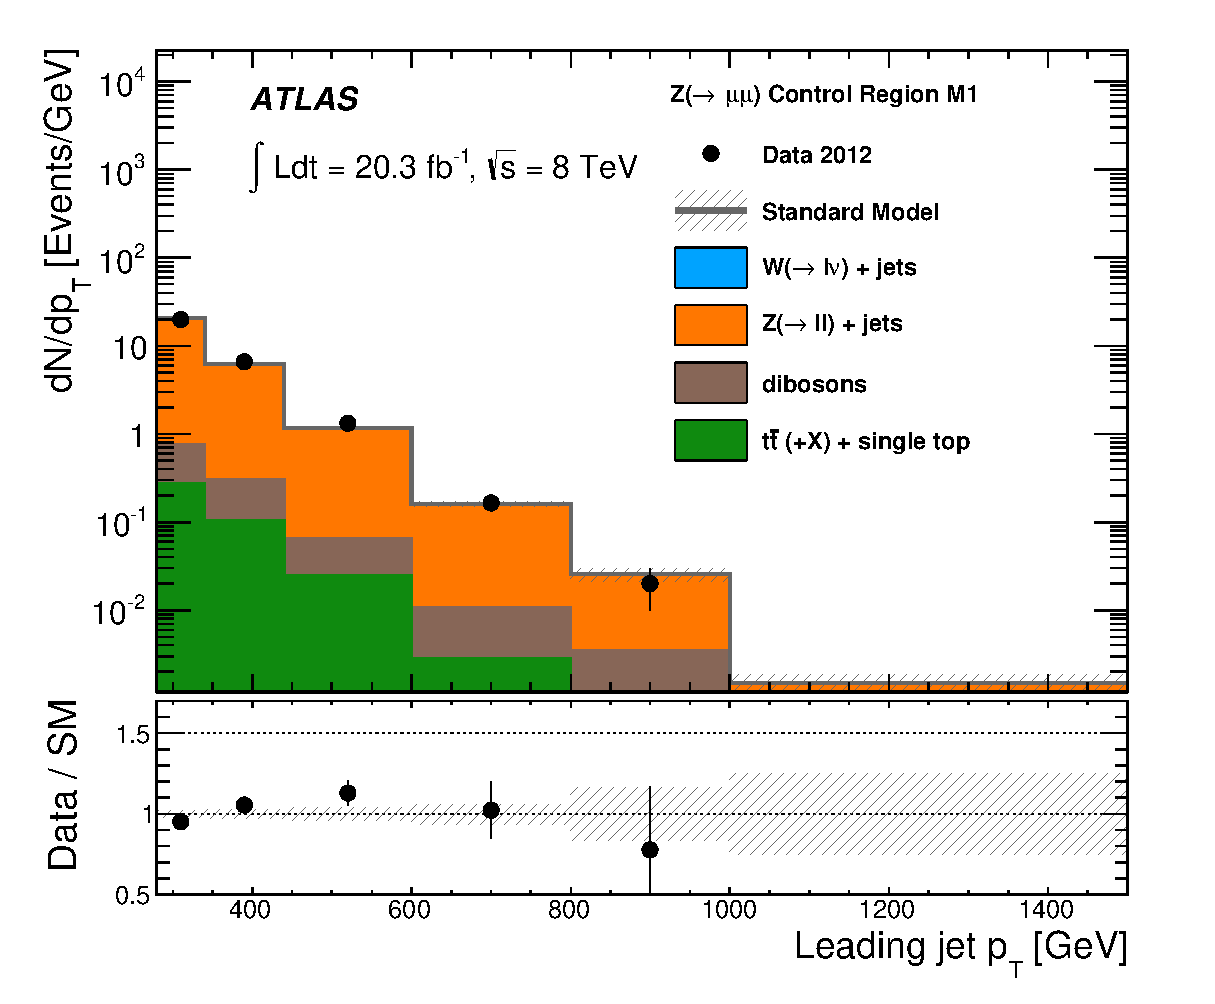
\includegraphics[width=0.495\textwidth]{MonojetAnalysis/Figures/plot_Stop_A6_CRzmm_pt1_fitted.eps}
      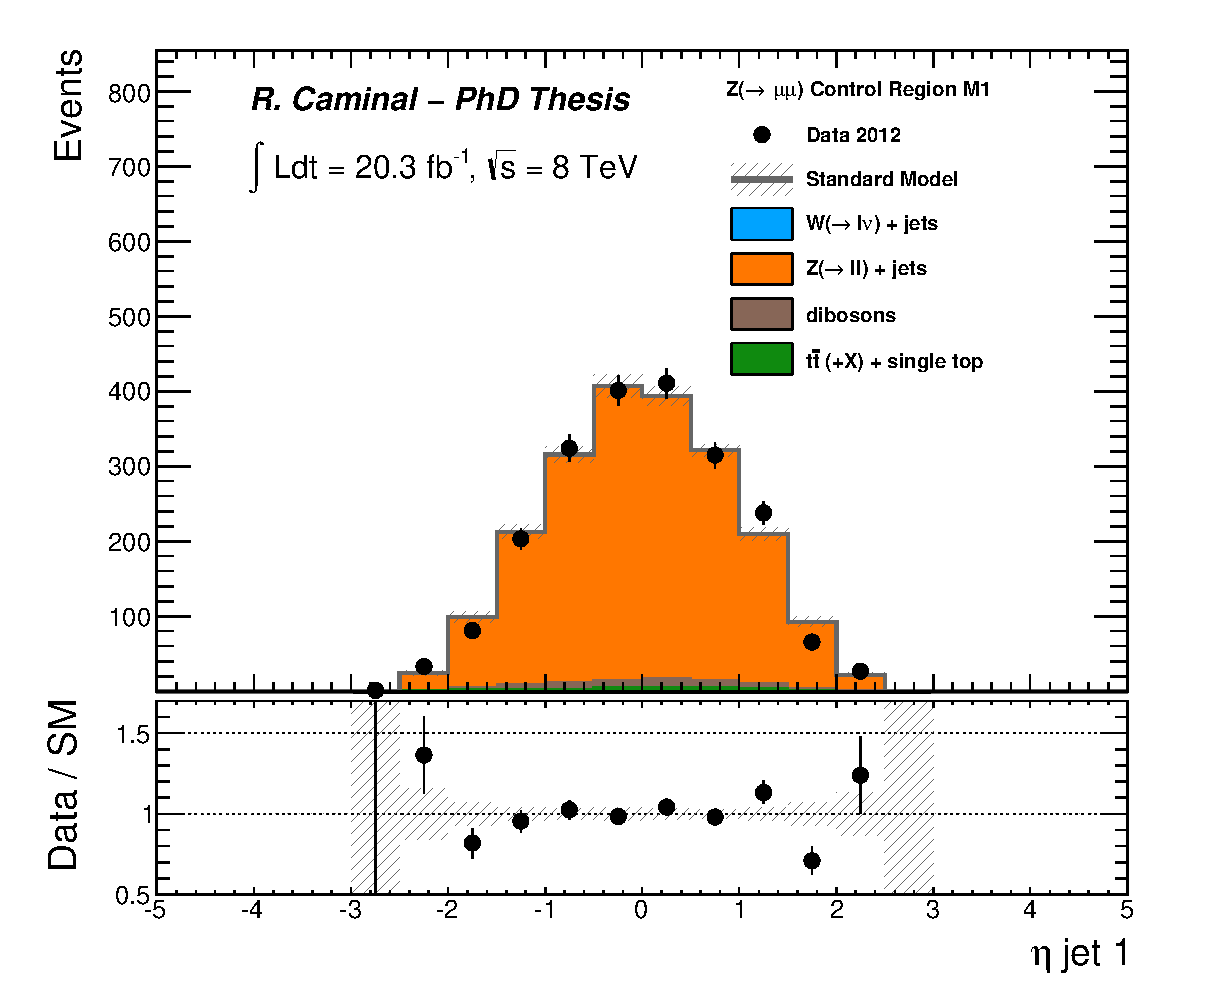
\includegraphics[width=0.495\textwidth]{MonojetAnalysis/Figures/plot_Stop_A6_CRzmm_eta1_fitted.eps}
    }
    \mbox{
      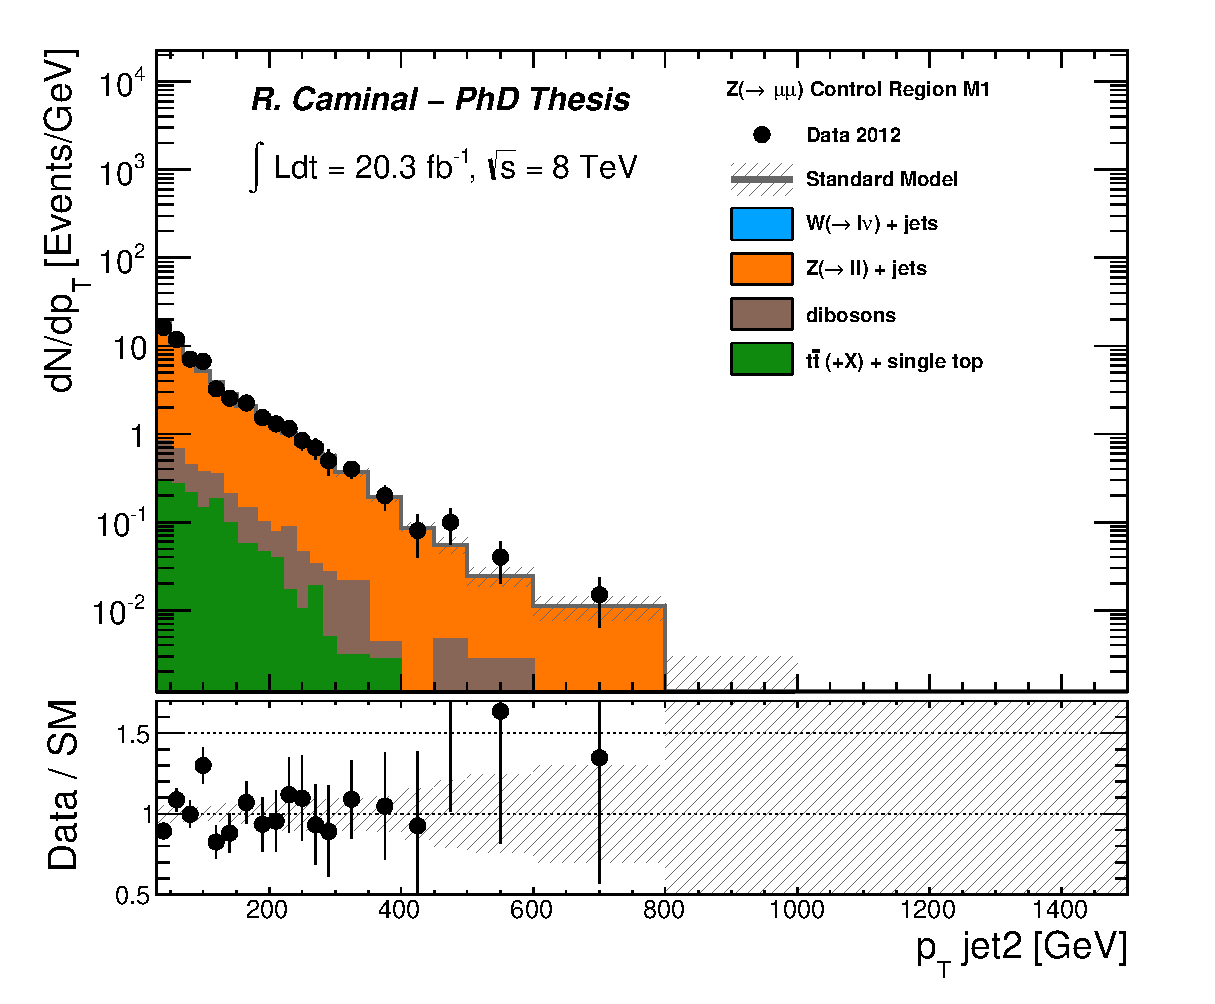
\includegraphics[width=0.495\textwidth]{MonojetAnalysis/Figures/plot_Stop_A6_CRzmm_pt2_fitted.eps}
      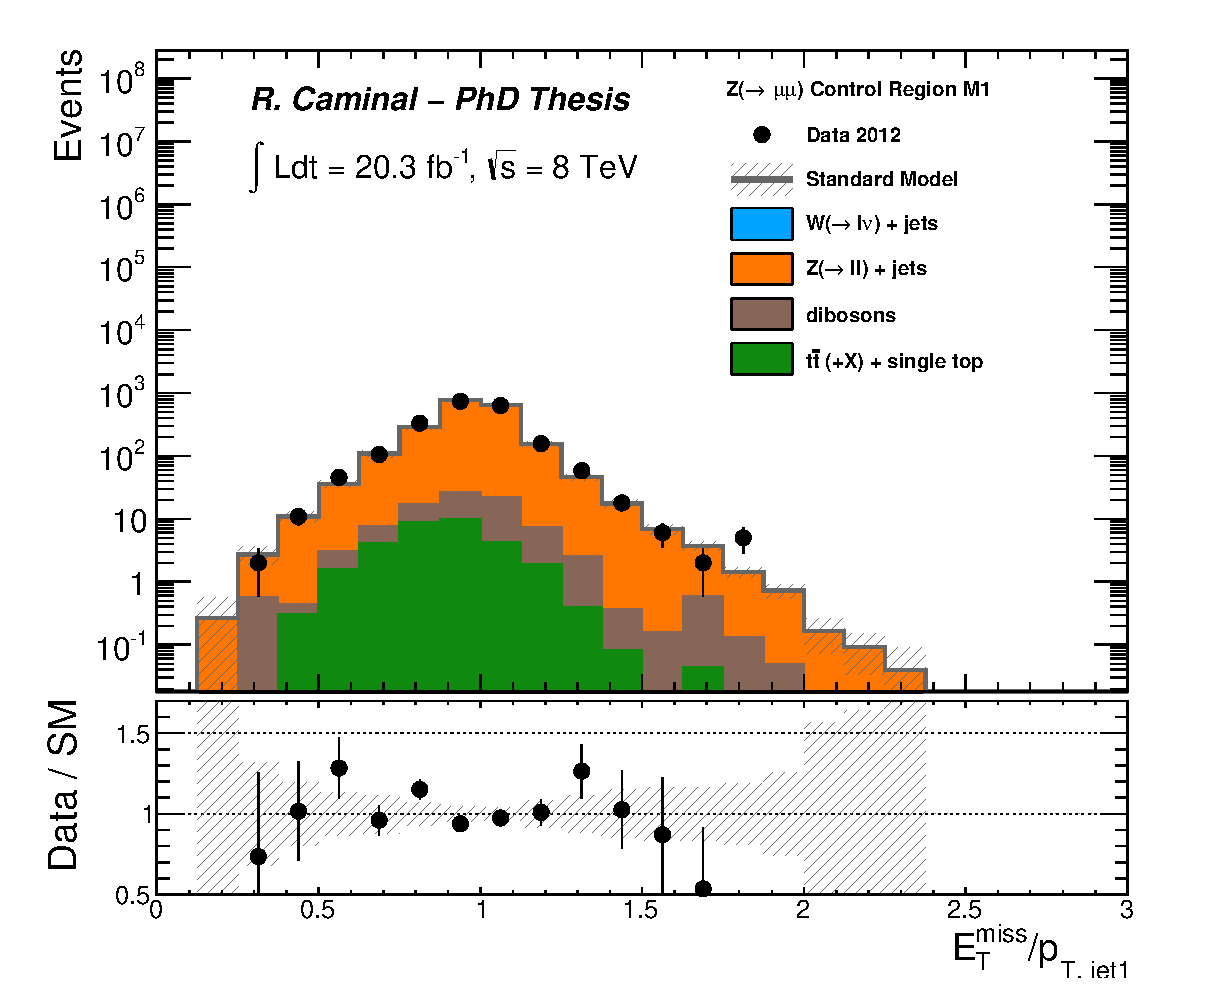
\includegraphics[width=0.495\textwidth]{MonojetAnalysis/Figures/plot_Stop_A6_CRzmm_metpt1_fitted.eps}
    }
  \end{center}
  \caption[Kinematic distributions of the reconstructed jets and $\met$ in the $\zmm$ control region for the selection cuts of region M1, after the normalization factors extracted from the fit have been applied.]{The measured kinematic distributions of the reconstructed jets and $\met$ in the $\zmm$ control region for the selection cuts of region M1 compared to the background predictions. The latter include the global normalization factors extracted from the fit. The error bands in the ratios include the statistical and experimental uncertainties on the background predictions.}
  \label{fig:Plot_M1_CRzmm_Jetkinematics}
\end{figure}

All the distributions show a reasonable agreement between data and MC in the control regions, thus pointing to a good modeling of the main SM background processes.


\clearpage
\section{Results}
    \label{sec:ResultsSR}

The agreement between the data and the MC simulations for the different distributions in the control regions of each selection shown in the previous section ensures the good modeling and control on the prediction of the main electroweak background processes in the signal regions.

As already mentioned, the global fit of the likelihood to the data in the different control regions, will translate into a reduction of the systematic effects.
Figures~\ref{fig:SystematicUncertaintiesSR} and \ref{fig:SystematicUncertaintiesSR2} summarize the systematic uncertainties for the signal regions M1 to M6 after the global fit.
Absolute jet and $\met$ energy scale and resolution systematic effects translate into an uncertainty on the total background that varies between 1.1\% and 1.4\% for M1-M4 and between 2.4\% and 2.1\% for M5 and M6 selections.
Uncertainties related to jet quality requirements and pileup description and corrections to the jet $\pt$ and $\met$ introduce a $0.2\%$ to $0.4\%$ uncertainty on the background predictions.
Uncertainties on the simulated lepton identification and reconstruction efficiencies, energy/momentum scale and resolution translate into a $0.9\%$ to $1.2\%$ for the different signal regions.

\begin{figure}[!ht]
  \begin{center}
    \mbox{
      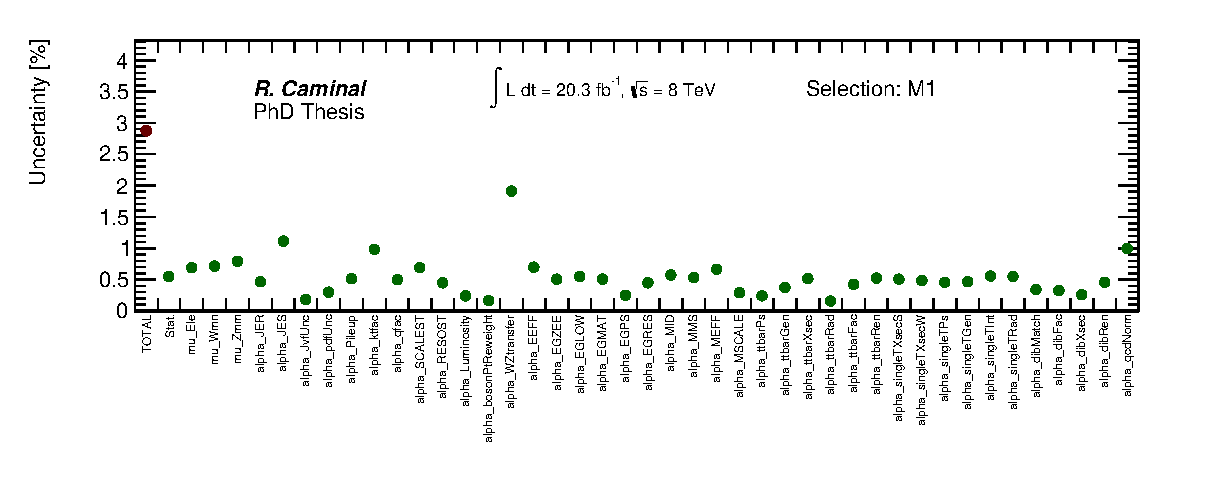
\includegraphics[width=0.995\textwidth]{MonojetAnalysis/Figures/totalSystematicPlot_SR_Stop_A6.eps}
    }
    \mbox{
      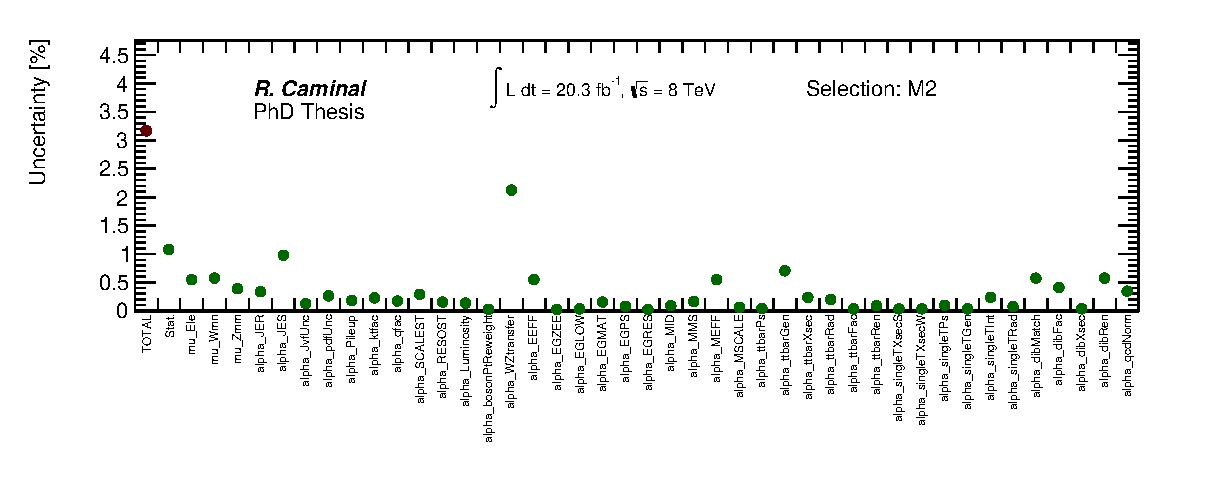
\includegraphics[width=0.995\textwidth]{MonojetAnalysis/Figures/totalSystematicPlot_SR_Stop_A3.eps}
    }
    \mbox{
      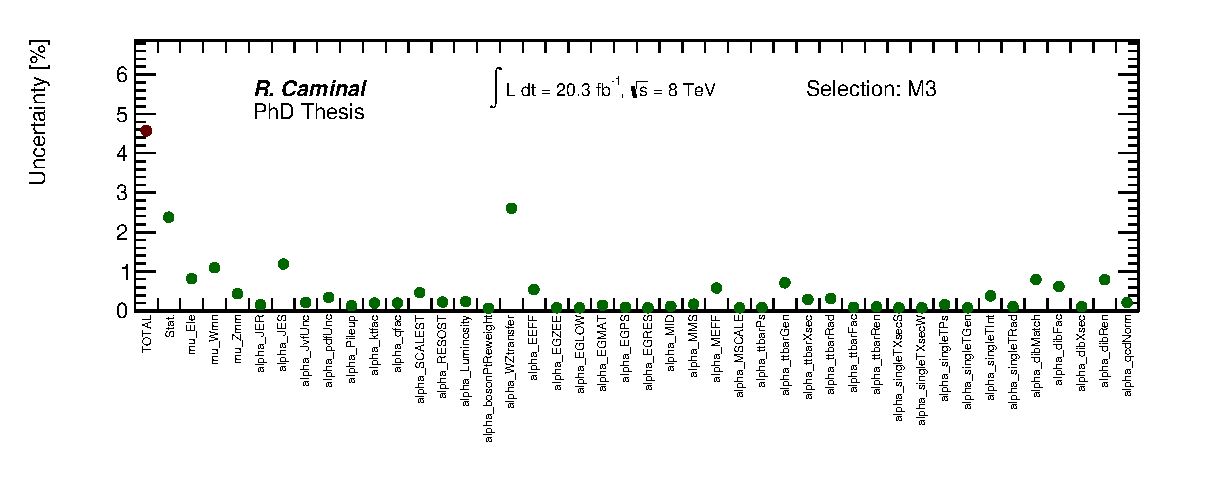
\includegraphics[width=0.995\textwidth]{MonojetAnalysis/Figures/totalSystematicPlot_SR_Stop_A4.eps}
    }
  \end{center}
  \caption[Breakdown of the sources of systematic uncertainties on background estimates in the M1 to M3 signal regions.]{Breakdown of the sources of systematic uncertainties on background estimates in the M1 to M3 signal regions. The first bin (in red) refers to the percentage of total systematic uncertainty with respect to the total background prediction. The individual uncertainties can be correlated, and therefore they do not necessarily add up quadratically to the total background uncertainty.}
  \label{fig:SystematicUncertaintiesSR}
\end{figure}


\begin{figure}[!ht]
  \begin{center}
    \mbox{
      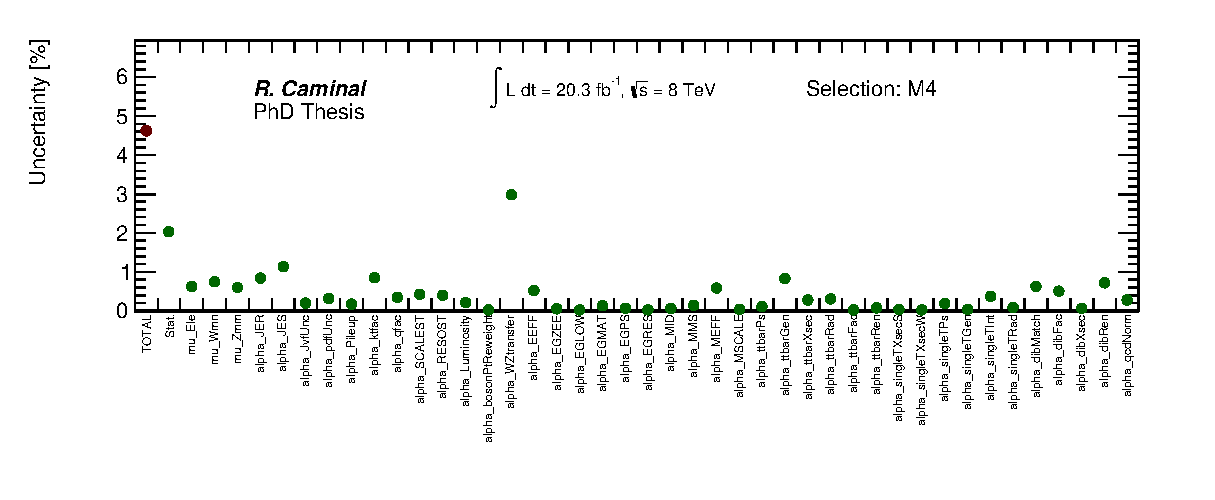
\includegraphics[width=0.995\textwidth]{MonojetAnalysis/Figures/totalSystematicPlot_SR_Stop_A8.eps}
    }
    \mbox{
      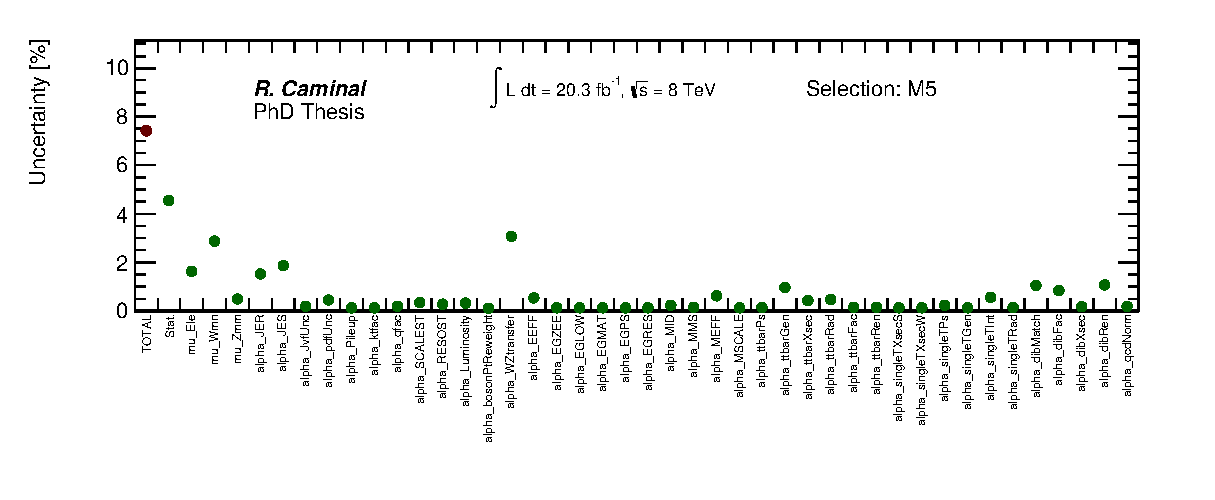
\includegraphics[width=0.995\textwidth]{MonojetAnalysis/Figures/totalSystematicPlot_SR_Stop_A9.eps}
    }
    \mbox{
      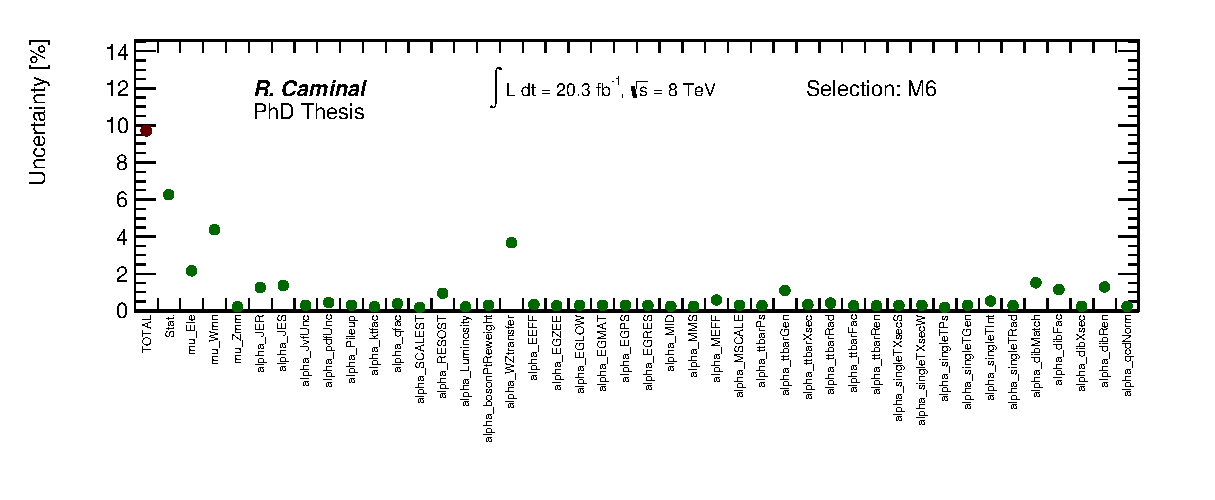
\includegraphics[width=0.995\textwidth]{MonojetAnalysis/Figures/totalSystematicPlot_SR_Stop_A10.eps}
    }
  \end{center}
  \caption[Breakdown of the sources of systematic uncertainties on background estimates in the M4 to M6 signal regions.]{Breakdown of the sources of systematic uncertainties on background estimates in the M4 to M6 signal regions. The first bin (in red) refers to the percentage of total systematic uncertainty with respect to the total background prediction. The individual uncertainties can be correlated, and therefore they do not necessarily add up quadratically to the total background uncertainty.}
  \label{fig:SystematicUncertaintiesSR2}
\end{figure}

Variations on the renormalization/factorization and parton-shower matching scales and PDFs in the \sherpa{} $W/Z$+jets background samples translate into a $0.4\%$ to $1\%$ uncertainty in the total background, while the effect of the boson $\pt$ re-weighting procedure for the simulated $W$ and $Z$ $\pt$ distributions introduces less than a $0.2\%$ effect on the total background estimates.
The model uncertainties related to potential differences between $W$+jets and $Z$+jets final states, affecting the normalization of the main irreducible background, $\znn$, are found to vary between about $2\%$ for M1 and $3\%$ for M2 to M6.
Theoretical uncertainties on the predicted background yields for top-quark-related processes is found to introduce an uncertainty on the total background between $1.0\%$ and $1.6\%$.
Uncertainties on the diboson affects the total background, between $0.7\%$ and $1.3\%$ for M1-M4, $1.7\%$ for M5 and $2.3\%$ for M6 selection.
The uncertainty on the multijet estimation leads to a $1\%$ uncertainty on the total background in M1, while it is negligible for the other selections.

Finally, the statistical uncertainties in the control regions in both data and MC are included in the analysis via the uncertainties quoted in the \texttt{mu\_Ele}, \texttt{mu\_Wmn} and \texttt{mu\_Zmm} normalization factors.
They lead to an additional uncertainty on the final background estimate that varies between $1.2\%$ and $1.4\%$ for M1-M4 selections, but is of the order of $4\%$ for M5 and M6.
The total uncertainty on the SM predictions varies between 2.9\% and 9.8\% in the different signal regions, and is summarized in Table~\ref{tab:SystematicSummary}.

\begin{table}[tb]
\begin{center}
\begin{small}
\begin{tabular}{cc}
\hline
\textbf{Selection} & \textbf{Total systematic uncertainty} \\ 
\hline
M1              & 2.9\% \\ 
M2              & 3.2\% \\ 
M3              & 4.6\% \\ 
M4              & 4.6\% \\ 
M5              & 7.4\% \\ 
M6              & 9.8\% \\ 
\hline
\end{tabular}
\end{small}
\end{center}
\renewcommand{\baselinestretch}{1}
\caption{Summary of the total systematic uncertainties on the SM predictions for the selections M1 to M6.}
\label{tab:SystematicSummary}
\end{table}

The background composition of the control and signal regions for each selection, after the global fit, is shown in Figure~\ref{fig:RegionsComposition}.
The first three bins for each selection refer to the $\wmn$+jets, $\wen$+jets and $\zmm$+jets control samples respectively (Tables~\ref{tab:ControlRegion_CRele} to \ref{tab:ControlRegion_CRzmm}).
Control samples are dominated by the background process from which they receive the name.
By construction, the agreement between the data and the MC simulation in the control samples is perfect, since these regions are used to constrain the backgrounds. 
The fourth bin refers to the signal region, where the irreducible $\znn$ process dominates, accounting for more than 50\% of the total background.
The relative contribution of this process in the different selections increases, as the leading jet $\pt$ and $\met$ requirements tighten.
The second most important process in the signal regions is the $\wtn$, due to the hadronically decaying $\tau$-leptons.
Further contributions come from $\wen$+jets and $\wmn$+jets processes, which pass the signal region requirements when the leptons are not reconstructed or are misreconstructed as jets.


\begin{figure}[!ht]
  \begin{center}
    \mbox{
      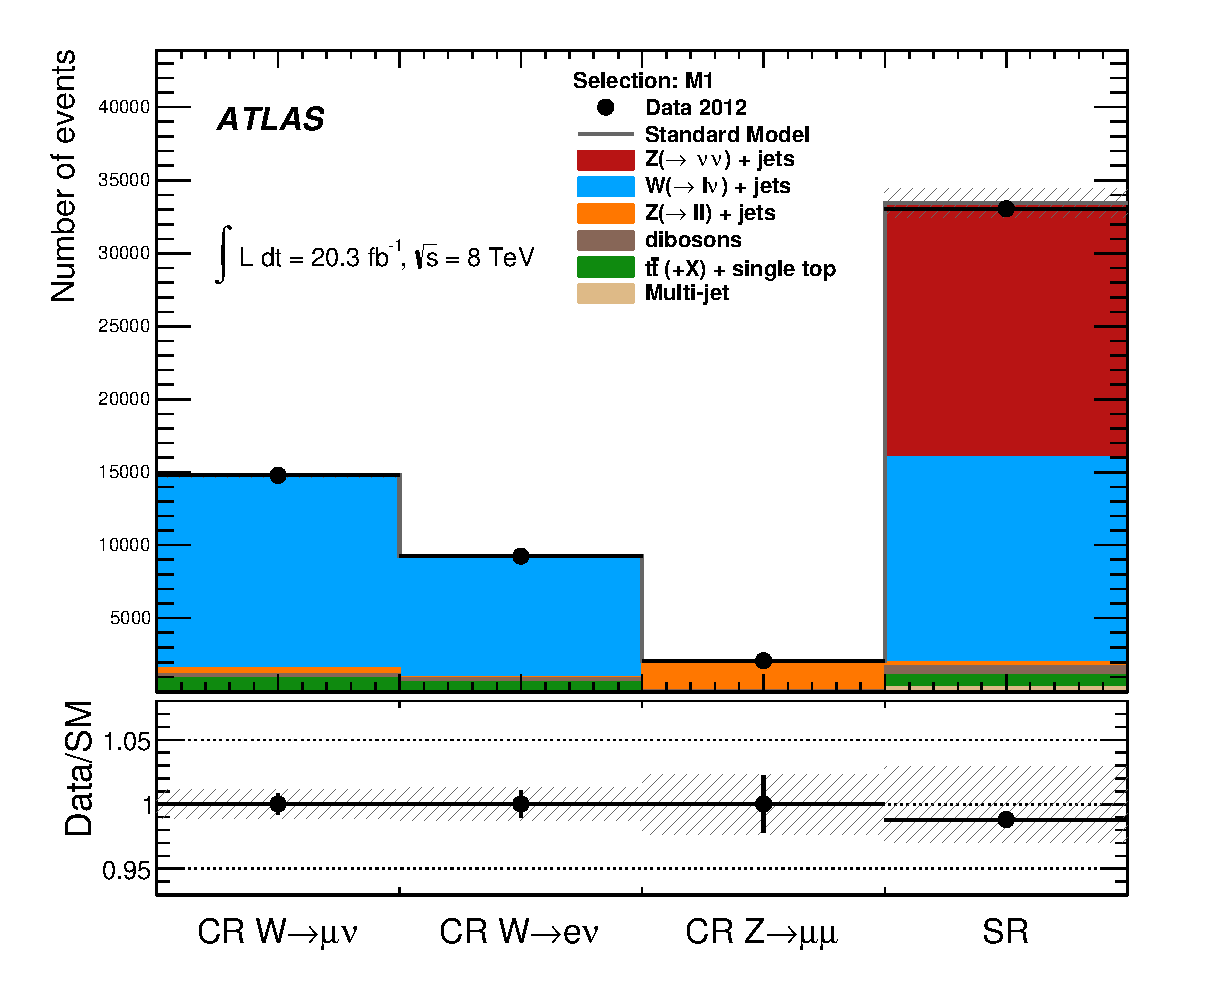
\includegraphics[width=0.495\textwidth]{MonojetAnalysis/Figures/regionsComposition_Stop_M1.eps}
      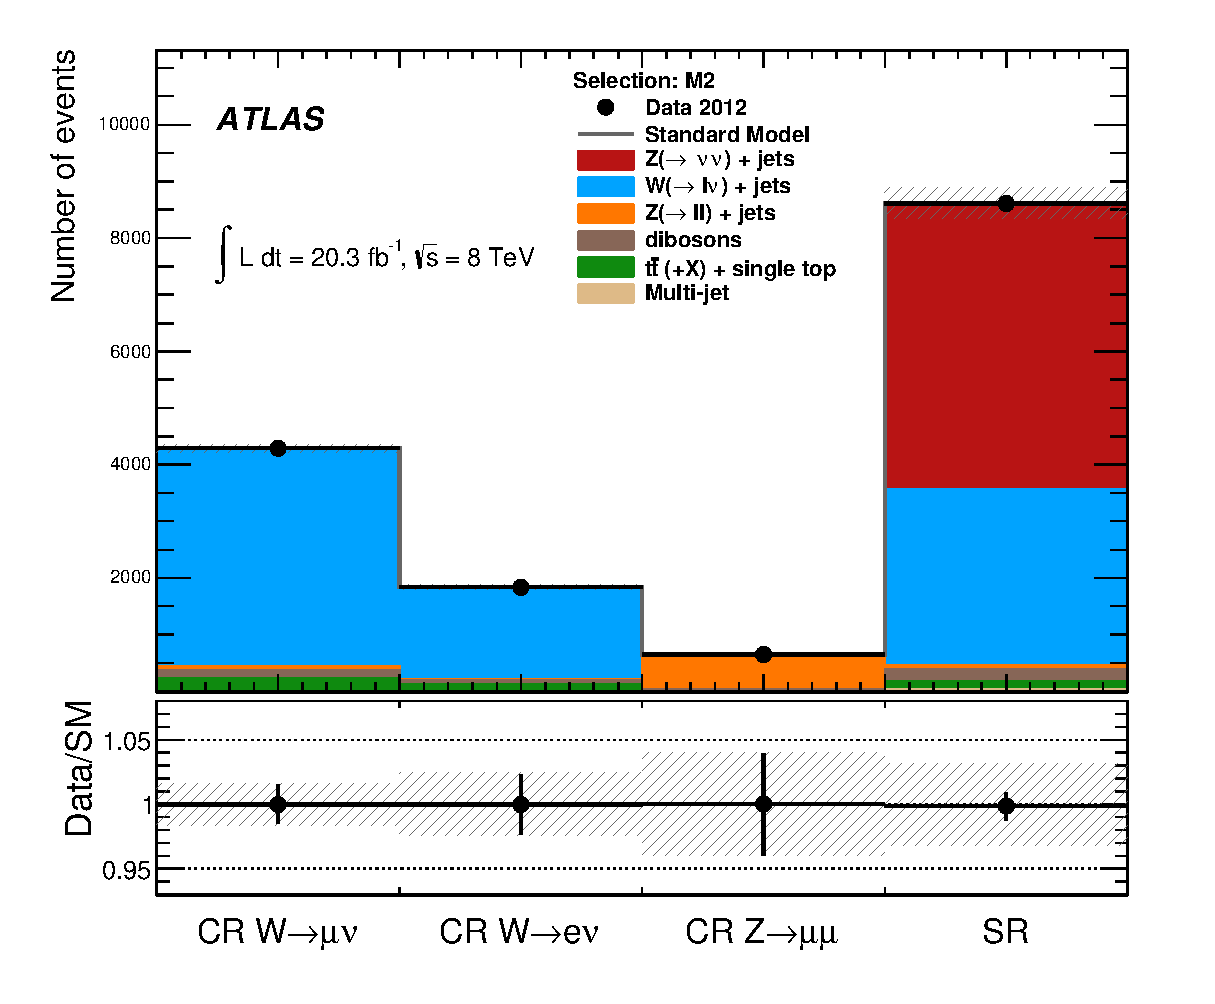
\includegraphics[width=0.495\textwidth]{MonojetAnalysis/Figures/regionsComposition_Stop_M2.eps}
    }
    \mbox{
      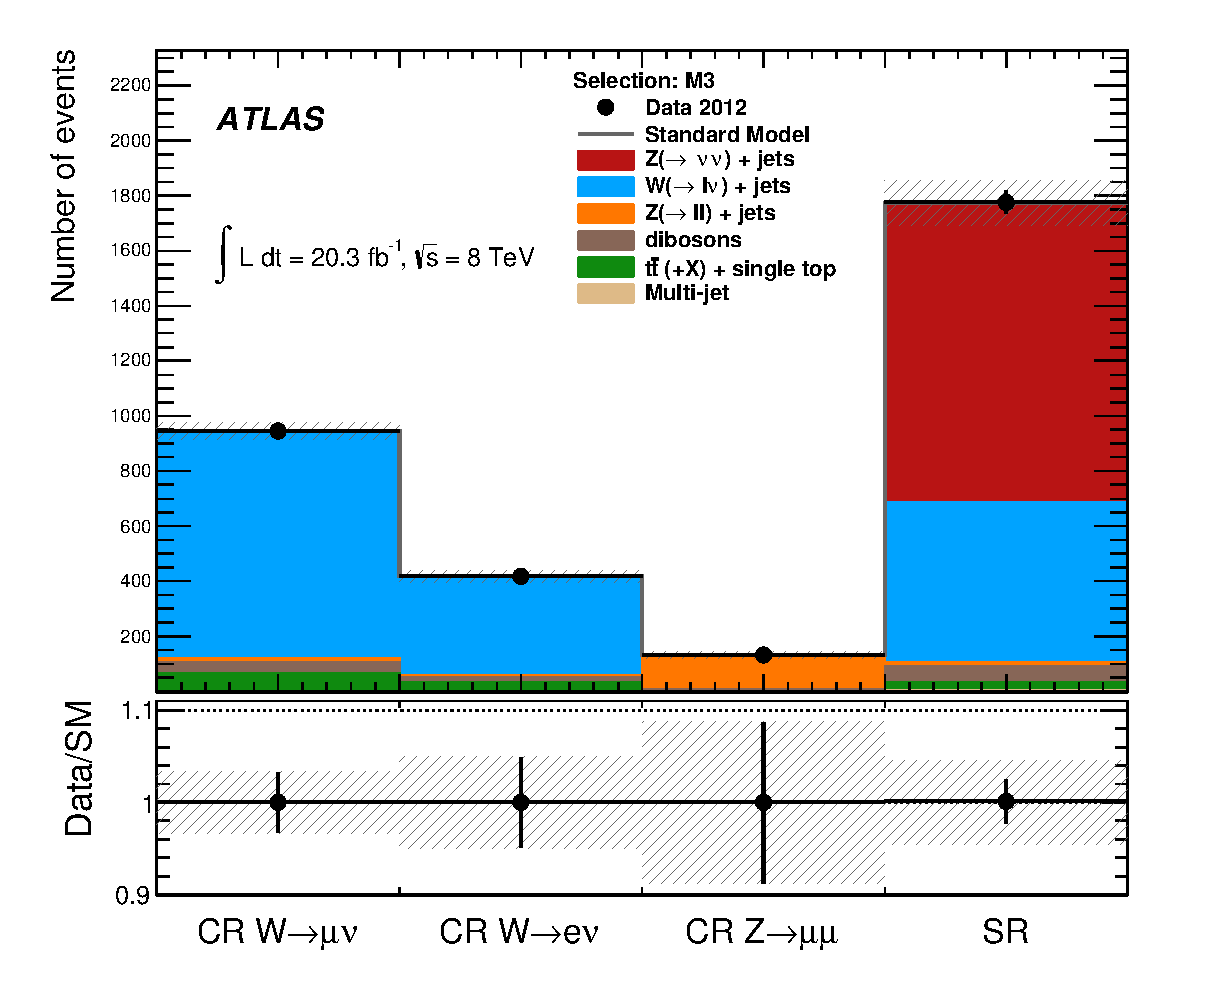
\includegraphics[width=0.495\textwidth]{MonojetAnalysis/Figures/regionsComposition_Stop_M3.eps}
      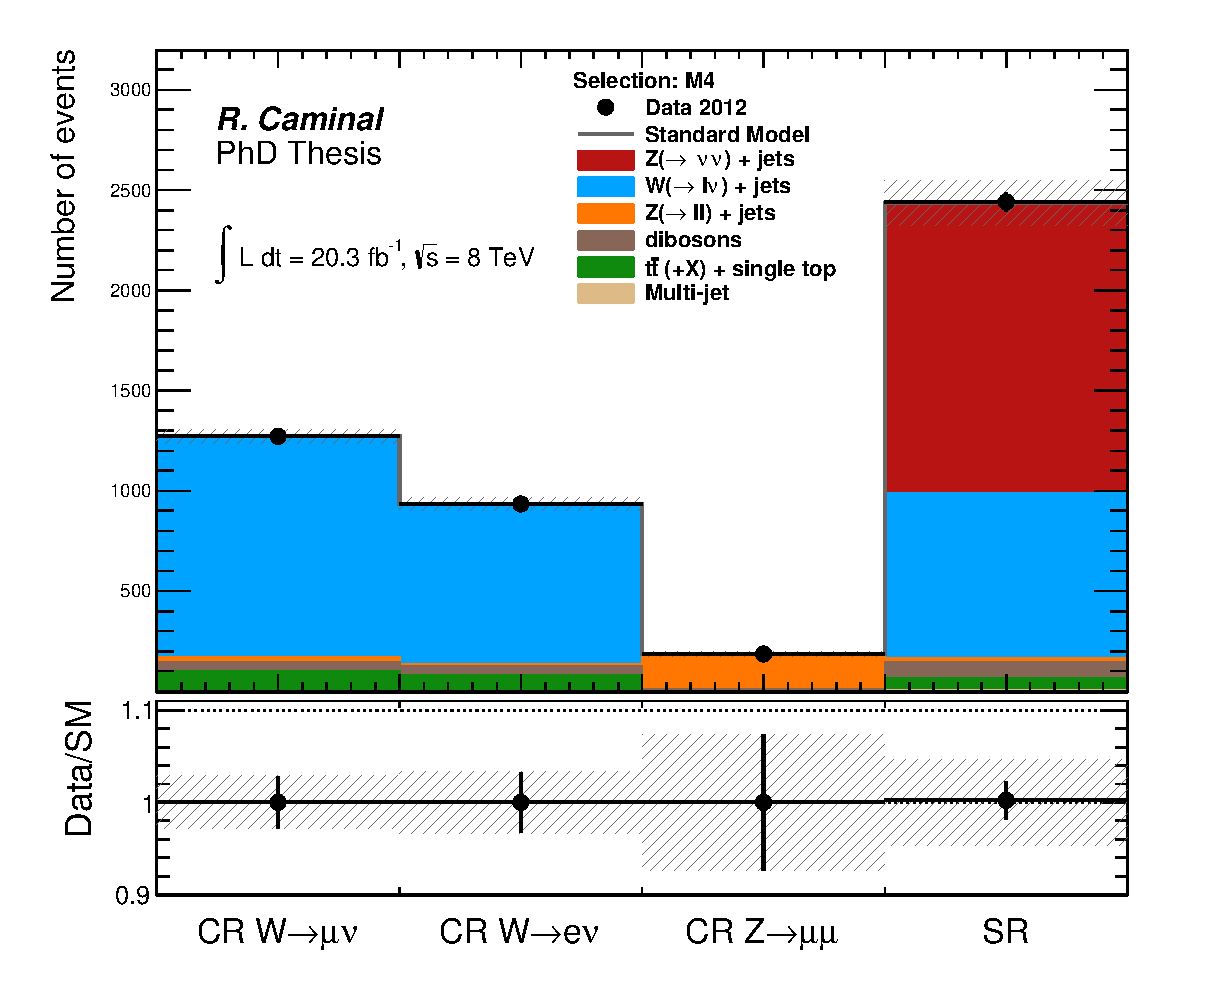
\includegraphics[width=0.495\textwidth]{MonojetAnalysis/Figures/regionsComposition_Stop_M4.eps}
    }
    \mbox{
      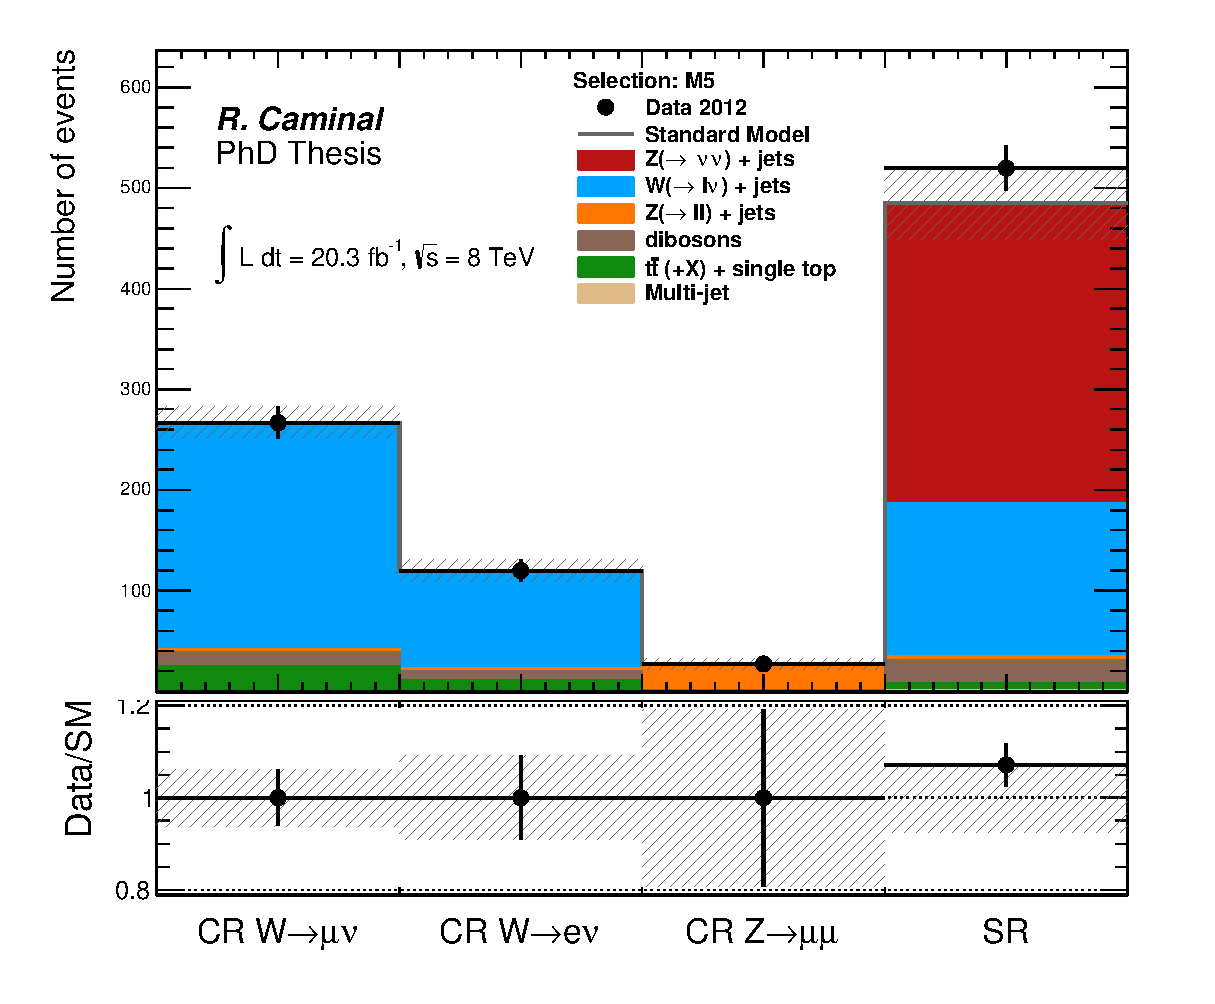
\includegraphics[width=0.495\textwidth]{MonojetAnalysis/Figures/regionsComposition_Stop_M5.eps}
      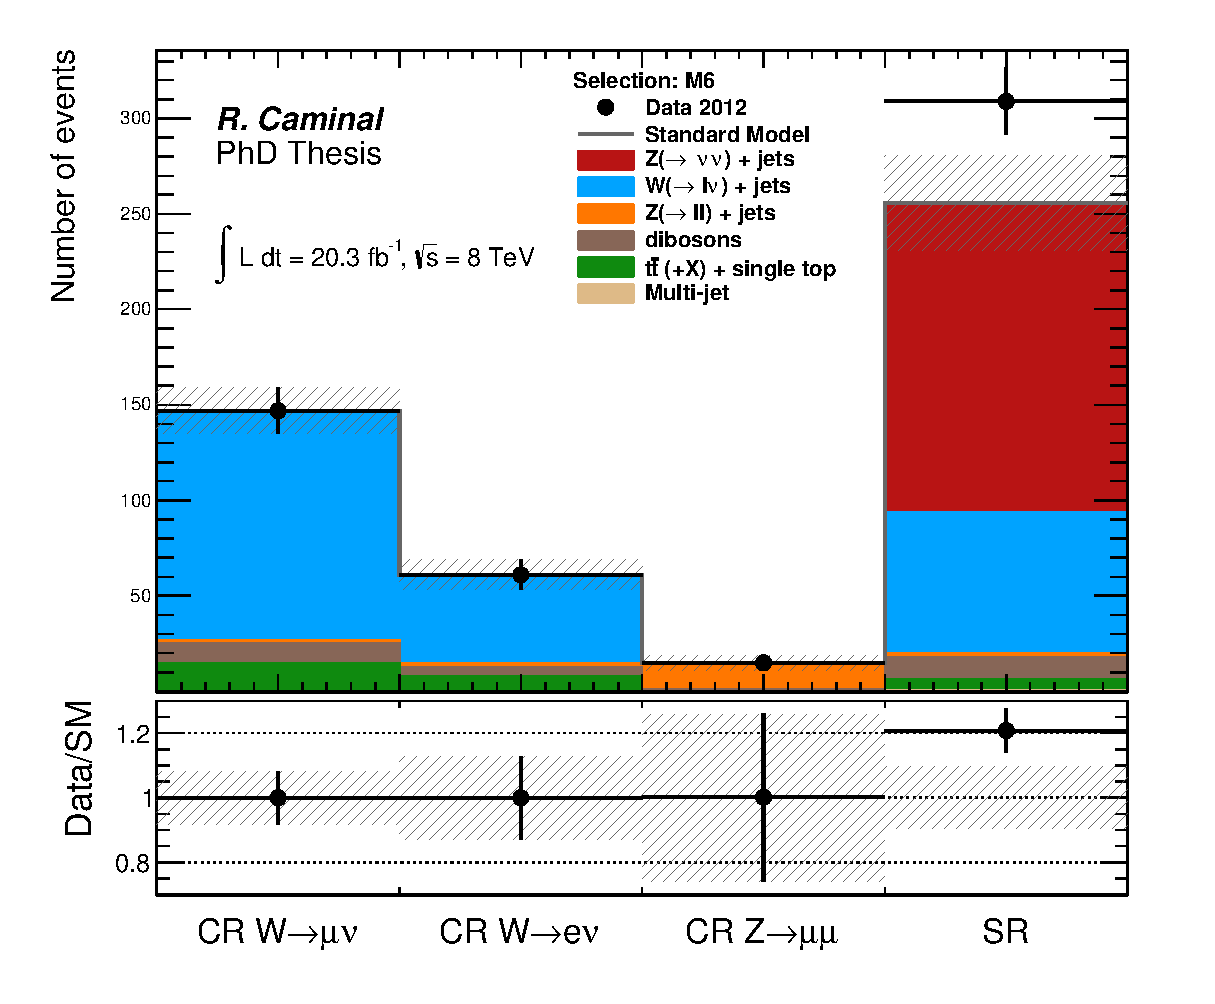
\includegraphics[width=0.495\textwidth]{MonojetAnalysis/Figures/regionsComposition_Stop_M6.eps}
    }
  \end{center}
  \caption[Background composition of the different control and signal regions for each of the kinematic selections after fits have been performed.]{Background composition of the different control and signal regions for each of the kinematic selections after fits have been performed. The error bands in the ratios include the total statistical and systematic uncertainties on the total background expectation. From top to bottom, left to right: M1-M6 selections.}
  \label{fig:RegionsComposition}
\end{figure}

Table~\ref{tab:SignalRegions} shows the data and the expected background predictions for signal regions M1 to M6.
Good agreement between the observed data and the simulation is observed between selections M1 to M5.
The selection M6 seems to show an excess of events with respect to the background estimation.
The compatibility between the data and the simulation under the hypothesis of having only background can be tested by computing the observed $p$-value, $p_b$, as described in detail in Chapter~\ref{chapter:StatisticalModel}.
Table~\ref{tab:pValuesBackgroundOnly} shows the $p$-values for the different signal selections.
The $p$-values for the regions M1 to M5 point to a good agreement between the data and the MC simulation, as previously discussed.
In the signal region M6, the data and the MC simulation agree within $2\sigma$.
This is studied in detail in Appendix~\ref{app:scaleFactorEvolution}, and is finally attributed to a statistical fluctuation in both the data and the MC events.

\begin{table}[!ht]
\begin{center}
\begin{small}
\begin{tabular*}{\textwidth}{@{\extracolsep{\fill}}lrrr}\hline
{\bf  Signal Region}  & \textbf{M1} & \textbf{M2} & \textbf{M3}  \\
    Observed events  (20.3 fb${}^{-1}$)&  $33054$  & $8606$  & $1776$   \\ \hline

    SM prediction (post-fit) &  $33450 \pm 960$  & $8620 \pm 270$ & $1770 \pm 81$  \\ \hline

    $\wen$+jets        &  $3300 \pm 140$ &  $700 \pm 43$   & $130 \pm 12$  \\

    $\wmn$+jets        &  $3000 \pm 100$ &  $700 \pm 29$  & $133 \pm 8$   \\

    $\wtn$        &  $7800 \pm 290$  & $1690 \pm 74$   & $320 \pm 24$  \\

    $\zee$+jets        &  $-$   &  $-$ & $-$  \\

    $\zmm$+jets        &  $170 \pm 27$  & $53 \pm 9$  & $13 \pm 3$  \\

    $\ztt$+jets        &  $95 \pm 6$    & $17 \pm 1$ & $1.8 \pm 0.3$ \\

    $\znn$        &  $17400 \pm 720$ & $5100 \pm 240$  &$1090 \pm 72$  \\ 

    $\ttbar$, single top          &     $780 \pm 73$   &  $150 \pm 19$ & $27 \pm 4$ \\

    Dibosons      &  $650 \pm 99$  & $220 \pm 40$  &  $60 \pm 14$  \\

    Multijets     &  $300 \pm 300$  & $30 \pm 30$  &  $4 \pm 4$  \\ \hline \hline

{\bf  Signal Region}  & \textbf{M4} & \textbf{M5} & \textbf{M6}  \\
    Observed events  (20.3 fb${}^{-1}$)&  $2441$ & $520$ & $309$ \\ \hline

    SM prediction (post-fit) &  $2435 \pm 113$ & $485 \pm 36$       & $256 \pm 25$ \\ \hline

    $\wen$+jets        &  $183 \pm 13$   & $33 \pm 5$         & $15 \pm 3$ \\

    $\wmn$+jets        &  $197 \pm 11$   & $36 \pm 4$         & $20 \pm 2$ \\

    $\wtn$        &  $445 \pm 26$   & $84 \pm 11$        & $40 \pm 8$ \\

    $\zee$+jets        &  $-$            & $-$                & $-$ \\

    $\zmm$+jets        &  $17 \pm 3$     & $3 \pm 1$          & $2 \pm 1$ \\

    $\ztt$+jets        &  $2.7 \pm 0.5$  & $0.6 \pm 0.1$      & $0.3 \pm 0.1$ \\

    $\znn$        &  $1446 \pm 99$  & $298 \pm 31$       & $162 \pm 22$ \\ 

    $\ttbar$, single top   & $58 \pm 8$ & $8 \pm 2$ & $6 \pm 1$ \\

    Dibosons      &  $81 \pm 19$    & $22 \pm 5$         & $12 \pm 3$ \\

    Multijets     &  $7 \pm 7$      & $0.7 \pm 0.7$     & $0.4 \pm 0.4$ \\ 
    
    \hline

    \end{tabular*}
    \end{small}

    \end{center}
    \caption[Data and SM background predictions in the signal regions M1 to M6.]
{Data and SM background predictions in the signal regions M1 to M6. 
      For the SM predictions both statistical and systematic uncertainties are included.
        Note that in each case the individual 
        uncertainties can be correlated, and do not necessarily add up quadratically to the total background uncertainty.
    }
\label{tab:SignalRegions}
\end{table}
 %--- \ref{tab:SignalRegions}

\begin{table}[tb]
\begin{center}
\begin{tabular}{cccccc}
\hline\hline
{\bf Signal channel} & & $\mathbf{p_b}$ \\
\hline
\multirow{2}{*}{M1} & asymp & $0.51$ \\
                    & toy   & $0.51$ \\
\multirow{2}{*}{M2} & asymp & $0.52$ \\
                    & toy   & $0.52$ \\
\multirow{2}{*}{M3} & asymp & $0.51$ \\
                    & toy   & $0.51$ \\
\multirow{2}{*}{M4} & asymp & $0.48$ \\
                    & toy   & $0.48$ \\
\multirow{2}{*}{M5} & asymp & $0.21$ \\
                    & toy   & $0.21$ \\
\multirow{2}{*}{M6} & asymp & $0.04$ \\
                    & toy   & $0.04$ \\
\hline\hline
\end{tabular}
\end{center}
\caption{$p$-values under the background-only hypothesis for the regions M1-M6, derived from pseudo-experiments (toy) and from an asymptotic approximation.}
\label{tab:pValuesBackgroundOnly}
\end{table}

\clearpage

Figures~\ref{fig:Plot_M1_SR_met} and~\ref{fig:Plot_M1_SR_pt1} show the $\met$ and the leading jet $\pt$ distributions in the signal regions M1 to M6, respectively.
Values for the $\met$ and leading jet $\pt$ up to $\unit[1.5]{TeV}$ are explored\footnote{No events are found with larger values of $\met$ or leading jet $\pt$.}.
Figure~\ref{fig:Plot_M1_SR_eta1} shows the pseudorapidity distribution of the leading jet in all the signal regions, and the distributions of the ratio between the $\met$ and the leading jet $\pt$ are shown in Figure~\ref{fig:Plot_M1_SR_metpt1}.
For illustration purposes, two different SUSY scenarios are included, for stop pair production in the $\stoptocharm$ decay channel with stop masses of $\unit[200]{GeV}$ and neutralino masses of $\unit[125]{GeV}$ and $\unit[195]{GeV}$.

The Standard Model predictions in all these distributions agree with the data, both in normalization and shape.
The predictions in the signal region M6, despite of the global $2\sigma$-level shift in the normalization, also show good agreement in the shape, which points to a statistical fluctuation, as mentioned above.
Other kinematic distributions of the reconstructed jets in the selections M1 to M6 are collected in Appendix~\ref{app:SRkimenaticDistr}.

\begin{figure}[!ht]
  \begin{center}
    \mbox{
      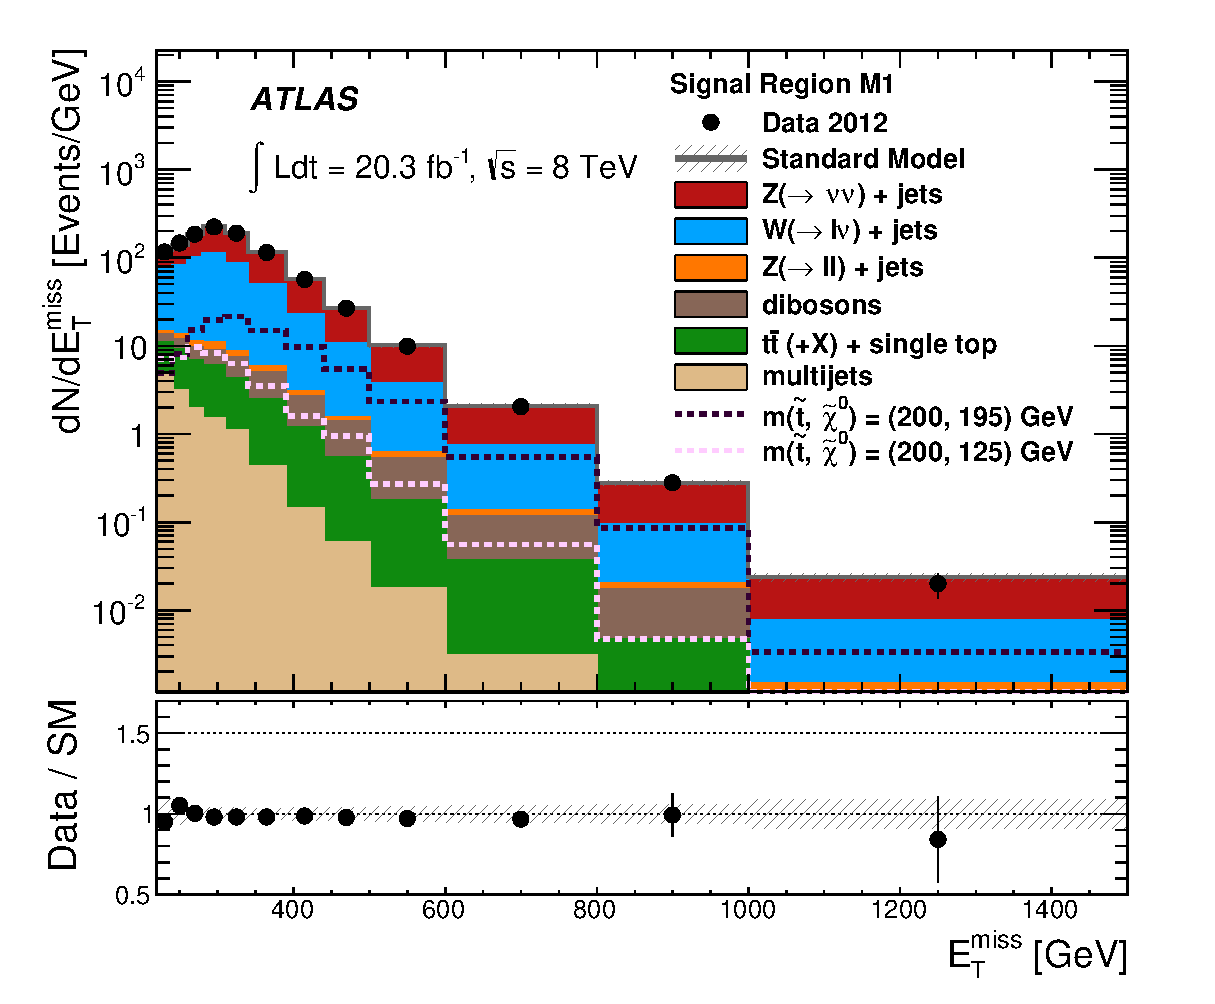
\includegraphics[width=0.495\textwidth]{MonojetAnalysis/Figures/plot_Stop_A6_SR_met_fitted.eps}
      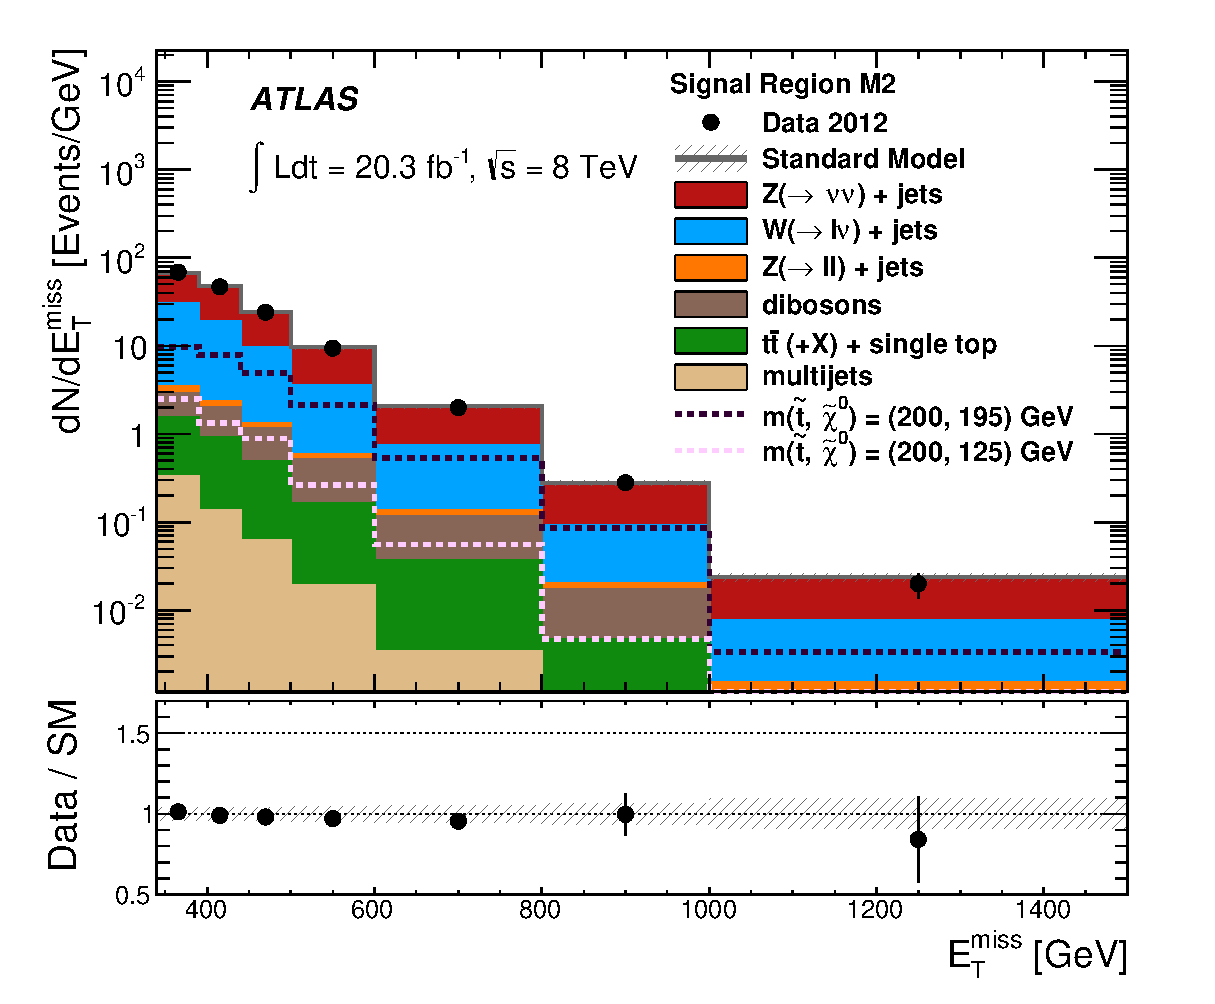
\includegraphics[width=0.495\textwidth]{MonojetAnalysis/Figures/plot_Stop_A3_SR_met_fitted.eps}
    }
    \mbox{
      \includegraphics[width=0.495\textwidth]{MonojetAnalysis/Figures/plot_Stop_A4_SR_met_fitted.eps}
      \includegraphics[width=0.495\textwidth]{MonojetAnalysis/Figures/plot_Stop_A8_SR_met_fitted.eps}
    }
    \mbox{
      \includegraphics[width=0.495\textwidth]{MonojetAnalysis/Figures/plot_Stop_A9_SR_met_fitted.eps}
      \includegraphics[width=0.495\textwidth]{MonojetAnalysis/Figures/plot_Stop_A10_SR_met_fitted.eps}
    }
  \end{center}
  \caption[Distributions of the reconstructed $\met$ in the signal regions for the selection cuts of regions M1 to M6, after the normalization factors extracted from the fit have been applied.]{The measured distributions of the reconstructed $\met$ in the signal regions for the selection cuts of regions M1 to M6 compared to the background predictions. The latter include the global normalization factors extracted from the fit. The error bands in the ratios include the statistical and experimental uncertainties on the background predictions. For illustration purposes, the distribution of two different SUSY scenarios for stop pair production are included.}
  \label{fig:Plot_M1_SR_met}
\end{figure}

\begin{figure}[!ht]
  \begin{center}
    \mbox{
      \includegraphics[width=0.495\textwidth]{MonojetAnalysis/Figures/plot_Stop_A6_SR_pt1_fitted.eps}
      \includegraphics[width=0.495\textwidth]{MonojetAnalysis/Figures/plot_Stop_A3_SR_pt1_fitted.eps}
    }
    \mbox{
      \includegraphics[width=0.495\textwidth]{MonojetAnalysis/Figures/plot_Stop_A4_SR_pt1_fitted.eps}
      \includegraphics[width=0.495\textwidth]{MonojetAnalysis/Figures/plot_Stop_A8_SR_pt1_fitted.eps}
    }
    \mbox{
      \includegraphics[width=0.495\textwidth]{MonojetAnalysis/Figures/plot_Stop_A9_SR_pt1_fitted.eps}
      \includegraphics[width=0.495\textwidth]{MonojetAnalysis/Figures/plot_Stop_A10_SR_pt1_fitted.eps}
    }
  \end{center}
  \caption[Distributions of the reconstructed $\pt$ of the leading jet in the signal regions for the selection cuts of regions M1 to M6, after the normalization factors extracted from the fit have been applied.]{The measured distributions of the reconstructed $\pt$ of the leading jet in the signal regions for the selection cuts of regions M1 to M6 compared to the background predictions. The latter include the global normalization factors extracted from the fit. The error bands in the ratios include the statistical and experimental uncertainties on the background predictions. For illustration purposes, the distribution of two different SUSY scenarios for stop pair production are included.}
  \label{fig:Plot_M1_SR_pt1}
\end{figure}


\begin{figure}[!ht]
  \begin{center}
    \mbox{
      \includegraphics[width=0.495\textwidth]{MonojetAnalysis/Figures/plot_Stop_A6_SR_eta1_fitted.eps}
      \includegraphics[width=0.495\textwidth]{MonojetAnalysis/Figures/plot_Stop_A3_SR_eta1_fitted.eps}
    }
    \mbox{
      \includegraphics[width=0.495\textwidth]{MonojetAnalysis/Figures/plot_Stop_A4_SR_eta1_fitted.eps}
      \includegraphics[width=0.495\textwidth]{MonojetAnalysis/Figures/plot_Stop_A8_SR_eta1_fitted.eps}
    }
    \mbox{
      \includegraphics[width=0.495\textwidth]{MonojetAnalysis/Figures/plot_Stop_A9_SR_eta1_fitted.eps}
      \includegraphics[width=0.495\textwidth]{MonojetAnalysis/Figures/plot_Stop_A10_SR_eta1_fitted.eps}
    }
  \end{center}
  \caption[Distributions of the reconstructed $\eta$ of the leading jet in the signal regions for the selection cuts of regions M1 to M6, after the normalization factors extracted from the fit have been applied.]{The measured distributions of the reconstructed $\eta$ of the leading jet in the signal regions for the selection cuts of regions M1 to M6 compared to the background predictions. The latter include the global normalization factors extracted from the fit. The error bands in the ratios include the statistical and experimental uncertainties on the background predictions. For illustration purposes, the distribution of two different SUSY scenarios for stop pair production are included.}
  \label{fig:Plot_M1_SR_eta1}
\end{figure}

\begin{figure}[!ht]
  \begin{center}
    \mbox{
      \includegraphics[width=0.495\textwidth]{MonojetAnalysis/Figures/plot_Stop_A6_SR_metpt1_fitted.eps}
      \includegraphics[width=0.495\textwidth]{MonojetAnalysis/Figures/plot_Stop_A3_SR_metpt1_fitted.eps}
    }
    \mbox{
      \includegraphics[width=0.495\textwidth]{MonojetAnalysis/Figures/plot_Stop_A4_SR_metpt1_fitted.eps}
      \includegraphics[width=0.495\textwidth]{MonojetAnalysis/Figures/plot_Stop_A8_SR_metpt1_fitted.eps}
    }
    \mbox{
      \includegraphics[width=0.495\textwidth]{MonojetAnalysis/Figures/plot_Stop_A9_SR_metpt1_fitted.eps}
      \includegraphics[width=0.495\textwidth]{MonojetAnalysis/Figures/plot_Stop_A10_SR_metpt1_fitted.eps}
    }
  \end{center}
  \caption[Distributions of the ratio between the reconstructed $\met$ and the leading jet $\pt$ in the signal regions for the selection cuts of regions M1 to M6, after the normalization factors extracted from the fit have been applied.]{The measured distributions of the reconstructed ratio between $\met$ and the leading jet $\pt$ in the signal regions for the selection cuts of regions M1 to M6 compared to the background predictions. The latter include the global normalization factors extracted from the fit. The error bands in the ratios include the statistical and experimental uncertainties on the background predictions. For illustration purposes, the distribution of two different SUSY scenarios for stop pair production are included.}
  \label{fig:Plot_M1_SR_metpt1}
\end{figure}
